\documentclass[11pt]{article}

\usepackage[margin=1.05in]{geometry}
\usepackage{amsmath,amssymb,amsthm}
\usepackage{mathtools}
\usepackage{graphicx}
\usepackage{booktabs}
\usepackage{array}
\usepackage{microtype}
\usepackage{xcolor}
\usepackage{tikz}
\usepackage[shortlabels]{enumitem}
\usepackage[colorlinks=true,linkcolor=blue!45!black,citecolor=blue!45!black,urlcolor=blue!45!black]{hyperref}
\hypersetup{pdftitle={The middle and the ends III. Face selection for slowly switching Markov chains and the planar persistent walk},pdfauthor={Arjun Pemmasani}}

% ---------- theorem environments ----------
\newtheorem{theorem}{Theorem}[section]
\newtheorem{lemma}[theorem]{Lemma}
\newtheorem{proposition}[theorem]{Proposition}
\newtheorem{corollary}[theorem]{Corollary}
\theoremstyle{definition}
\newtheorem{definition}[theorem]{Definition}
\newtheorem{example}[theorem]{Example}
\theoremstyle{remark}
\newtheorem{remark}[theorem]{Remark}

% ---------- notation macros ----------
\newcommand{\Z}{\mathbb{Z}}
\newcommand{\R}{\mathbb{R}}
\newcommand{\E}{\mathbb{E}}
\newcommand{\Prob}{\mathbb{P}}
\newcommand{\Var}{\operatorname{Var}}
\newcommand{\Cov}{\operatorname{Cov}}
\newcommand{\supp}{\operatorname{supp}}
\newcommand{\ones}{\mathbf{1}}
\newcommand{\tree}{\operatorname{tree}}

\graphicspath{{figures/}{../figures/}}

\title{The middle and the ends III.\\ Face selection for slowly switching Markov chains
 and the planar persistent walk}
\author{Arjun Pemmasani}
\date{September 26, 2026}
\begin{document}
\maketitle

\begin{abstract}
On Kagey's persistent Galton board each bounce repeats the previous one with
probability $p$, and Kagey asked when the middle bin becomes as likely as an
endpoint. We ask the same question for a Markov chain on $d$ states run for
$N$ steps, which jumps from state $i$ to state $j$ with probability
$q_{ij}T/N$. The bin is now the vector of visit counts. Write $T=\tau\log N$ and
let $\lambda_F$ be the rate at which the chain leaves a set of states $F$. To
first order the most likely count vector is supported by a set $F$ that
minimizes $\tau\lambda_F+\lvert F\rvert-1$: staying on $F$ costs
$N^{-\tau\lambda_F}$, and spreading over $F$ costs a factor $N$ per extra state.
At second order a local limit theorem gives a crossing equation in which
$\log\log N$ has the coefficient $\frac12$ for strongly connected sets with
start mass, and a directed 3-cycle shows that this can fail otherwise. Our main
application is the persistent walk on the square lattice that turns with rate
$r$ to each side and reverses with rate $s$. The corner and the origin are
equally likely exactly once, when $T/\log N$ is close to $\min(2/(2r+s),1/s)$,
and when reversals dominate the crossing is the 1-dimensional one for $N/2$
steps. We also treat sticky priors for hidden Markov models and the information in
the endpoint.
\end{abstract}

\noindent\textbf{Keywords:} persistent random walk; correlated random walk;
Galton board; occupation times of Markov chains; mode; principal Dirichlet
eigenvalue; quasi-stationary distribution; local limit theorem; Ising chain;
hidden Markov model.

\noindent\textbf{MSC2020:} 60J10; 60F05; 82B20; 60F10; 60G50; 62M05.

\section{Introduction}\label{sec:intro}

Suppose you drop a ball through a Galton board with $N$ rows of pegs. At the
first peg the ball goes left or right with probability $\frac12$. At every
later peg it repeats its previous direction with probability $p$ and switches
with probability $q=1-p$. Problem~131 of Kagey's Open Problem
Collection~\cite{kagey131} asks for the law of the bin where the ball lands,
and in particular when the middle bin is exactly as likely as an endpoint. An
endpoint is reached by a single path, the one that never switches, so it has
probability $\frac12p^{N-1}$. When $p$ is close to $1$ this path wins, and when
$p$ is smaller the middle wins. Paper~A of this series~\cite{paperA} answers the
question at every $N$. The 2 are equally likely when the expected number of
switches $T=Nq$ is close to $\log N$. More precisely, the crossing value
$z_N$ of $T$ satisfies $z_N+\frac12\log z_N=\log N+\frac12\log\frac\pi8+o(1)$.

Kagey also asks what changes on other boards. In this paper the ball can move
in more than 2 directions. Our main example is Kagey's board in 2 dimensions.
A ball moves on the square lattice $\Z^2$, one step east, north, west or south
at a time. It starts in a uniform direction, and at each step it keeps its
direction, turns left or right, or reverses. Turns and reversals are rare: a
turn to each side has probability $rT/N$ and a reversal has probability $sT/N$.
After $N$ steps, which is more likely: the corner $(N,0)$, which only the path
that never turns can reach, or the origin? We show that for every even $N\ge4$
there is exactly one value $T^*_N$ of $T$ at which the 2 are equally likely,
and that
\[
 \frac{T^*_N}{\log N}\to\min\Bigl(\frac2{2r+s},\frac1s\Bigr)
\]
(Proposition~\ref{prop:decomp} and Theorem~\ref{thm:planar-first}). When
reversals dominate ($s>2r$) the origin is reached mostly by paths that stay on
one axis, and then $sT^*_N$ is the crossing $z_{N/2}$ of Kagey's board with
$N/2$ steps, up to $O(N^{-\gamma})$ (Theorem~\ref{thm:planar-rev}). When turns
dominate ($s<2r$) the origin is reached mostly by paths that use all 4
directions.

\subsection{Face selection}\label{sec:intro-faces}

The planar result is an instance of a general principle, which is the main
subject of this paper. Let the direction be a Markov chain on $d$ states that
switches from state $i$ to state $j$ with probability $q_{ij}T/N$ at each step,
and count the visits to each state. This count vector, the
\emph{composition}, plays the role of the bin. Its support is a set $F$ of
states, which we call a \emph{face} (it indexes a face of the simplex of
visit fractions). Which face carries the most likely composition, and at which
$T$ does the mode move to another face? On Kagey's board there are 2 states,
the faces of 1 state are the 2 endpoints and the face of 2 states is the set of
interior bins.

Put $T=\tau\log N$ and let $\lambda_F$ be the rate at which the chain leaves
$F$, that is, the principal Dirichlet eigenvalue on $F$ of $-Q$, where $Q$ is
the matrix of the rates $q_{ij}$. How likely the best composition with
support $F$ is depends on 2 effects.
\begin{itemize}
\item \emph{The cost of staying.} The chain must stay inside $F$ for all $N$
steps. This has probability about $e^{-T\lambda_F}=N^{-\tau\lambda_F}$. A
larger face is harder to leave, so staying on it is cheaper.
\item \emph{The cost of spreading.} The mass of $F$ is shared among the
compositions with support $F$, and there are about $N^{\lvert F\rvert-1}$ of
them, one factor $N$ for each free coordinate. Up to powers of $\log N$, the
best single composition gets a share $N^{-(\lvert F\rvert-1)}$.
\end{itemize}
So the most likely composition with support $F$ has probability
$N^{-\Phi_\tau(F)+o(1)}$, where
\[
 \Phi_\tau(F)=\tau\lambda_F+\lvert F\rvert-1,
\]
and every mode sits on a face that minimizes $\Phi_\tau$
(Theorem~\ref{thm:first}). In words, a sticky walk prefers a well-separated
community, a set of states that is hard to leave for its size. As $\tau$ grows
the cost of staying counts for more, and the mode moves to larger faces. On
Kagey's board an endpoint has $\Phi_\tau=\tau$ and the interior has
$\Phi_\tau=1$, so the middle takes over at $\tau=1$, which is the first-order
form of the answer of Paper~A. Section~\ref{sec:worked} works out 4 states on
a cycle by hand, and Theorem~\ref{thm:hull} reads the winners off the convex
hull of the points $(\lambda_F,\lvert F\rvert-1)$.

The planar walk fits this picture. The corner is the face of the single
direction east, with exit rate $2r+s$, so it has probability about
$N^{-(2r+s)\tau}$. The origin is reached either along an axis, with exit rate
$2r$, or with all 4 directions, with exit rate $0$. Comparing the 3 exponents
gives the limit above (Section~\ref{sec:planar}).

First order fixes the crossing only up to a factor $1+o(1)$. To locate it up to
$o(1)$ we need the constant in front. Say that a face $F$ satisfies (H) if the
chain can move between any 2 states of $F$ without leaving $F$, and the start
gives $F$ positive mass. For such faces we prove a local limit theorem inside
the face (Theorem~\ref{thm:local}). It shows (Theorem~\ref{thm:facemax}) that
the best composition with support $F$, with $k=\lvert F\rvert$ states, has
probability
\[
 M_F=N^{-(k-1)}\,T^{(k-1)/2}K_F\,e^{-T\lambda_F}\bigl(1+O(1/T+T^2/N)\bigr)
\]
uniformly for $1\le T\le N^{1/3}$, with an explicit constant $K_F$. The factor
$T^{(k-1)/2}$ appears because the visit fractions fluctuate on the scale
$T^{-1/2}$ in each of the $k-1$ free directions. Now let $F$ and $G$ satisfy
(H), and suppose that $F$ has $\Delta\ge1$ more states than $G$ and an exit rate
smaller by $\delta>0$. Then for large $N$ every $T\in[1,N^{1/3}]$ with $M_F=M_G$ satisfies
\[
 \delta T+\frac\Delta2\log T=\Delta\log N-\log\frac{K_F}{K_G}
 +O\Bigl(\frac1{\log N}\Bigr)
\]
(Theorem~\ref{thm:crossing}). So the coefficient $\frac12$ of $\log\log N$ that
Papers~A and~B found holds for every such pair, whatever the graph, the rates,
the sizes or the start, and without reversibility. For reversible faces $K_F$
involves the square root of a weighted count of spanning trees
(Proposition~\ref{prop:constant}), and the constants of Papers~A and~B are short
corollaries (Corollaries~\ref{cor:paperA} and~\ref{cor:paperB}). Without (H)
the coefficient can change. On a directed 3-cycle it is $1$ at one crossing and
$0$ at the next (Proposition~\ref{prop:threecycle}). Section~\ref{sec:examples}
computes all the constants on the 4-cycle, shows that the start can decide which
face wins, and lists the winners on other graphs.

The paper closes with 2 applications, and nothing before them depends on them.
Section~\ref{sec:sticky} applies face selection to sticky priors for hidden
Markov models, and Section~\ref{sec:fisher} asks how much of the Fisher
information about the switching rate is left when we only see the bin of
Kagey's board. Section~\ref{sec:model} fixes the notation,
Section~\ref{sec:verify} describes the computer checks and open questions, and
the longer proofs are in the appendices.

\subsection{The series}\label{sec:series}

This is the third of 4 papers on Problem~131, \emph{The middle and the ends
I--IV}. We call them Papers~A to~D, so that Paper~A~\cite{paperA} is part~I,
Paper~B~\cite{paperB} is part~II, this paper is part~III and
Paper~D~\cite{paperD} is part~IV. They share the following notation.
\begin{itemize}[leftmargin=1.5em,itemsep=1pt,topsep=3pt]
\item Kagey's board has $N$ steps (his row $n$ has $N=n-1$). The first step is
left or right with probability $\frac12$, and each later step repeats the
previous one with probability $p$. We write $q=1-p$ and $u=q/p$, the odds of a
switch.
\item $P_N(k)$ is the probability of $k$ right steps, that is, that the ball
lands in bin $k$. The endpoints have $P_N(0)=P_N(N)=p^{N-1}/2$.
\item $L=\log N$, and $T=Nq$ is the expected number of switches (up to the
first step).
\item The crossing is the value of $p$ (or $T$) at which a bin is exactly as
likely as an endpoint. For the middle bin it is $p_N$, and $z_N=N(1-p_N)$.
\item With $d$ states, a face $F$ is a nonempty set of states, and the vertices
are the faces of size $1$. $\lambda_F$ is the principal Dirichlet eigenvalue of
$-Q$ on $F$, and $K_F$ is the second-order constant.
\end{itemize}
Paper~A solves Kagey's board: uniform Bessel bounds bracket $z_N$ for every
$N\ge2$ and give $z_N+\frac12\log z_N=L+c_0+1/(8z_N)+R_N$ with
$c_0=\frac12\log(\pi/8)$ and an explicit $R_N$. Paper~B lets the ball switch to
each of $d-1$ other directions at the same rate; there every face ties at first
order, and constants $a_k$ break the tie at second order. Paper~D asks what
memory changes. The present paper treats every rate matrix $Q$. It explains
which face carries the mode and why, computes the constants $K_F$, recovers
$c_0$ and $a_k$ as special cases, and applies all this to the planar walk.
Figure~\ref{fig:program} compares the crossings of the 4 papers.

\begin{figure}[t]
\centering
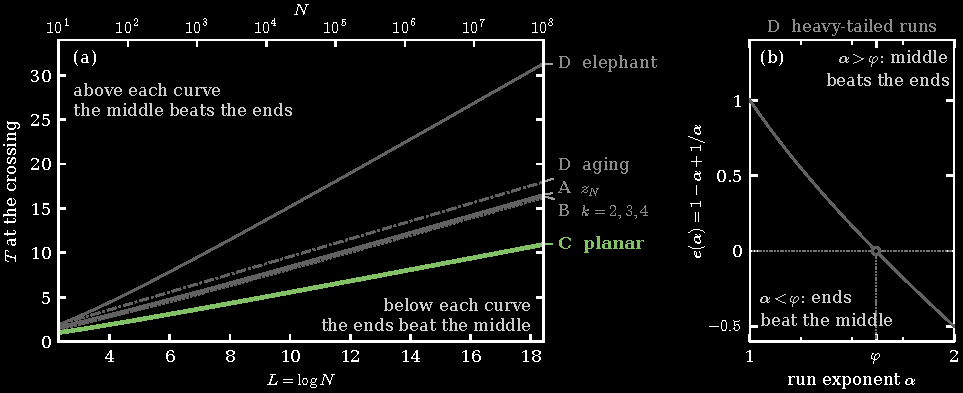
\includegraphics[width=\textwidth]{program_C}
\caption{(a) The crossing on each model's switching scale against $L=\log N$
for Papers~A to~D. The scale is $T$ for Papers~A to~C, $x=n\varepsilon$ for the
elephant walk and the expected number of switches for the aging walk of
Paper~D. The bold curve solves the first crossing equation of
Remark~\ref{rem:planar-turns} for the planar walk with $r=s=1$, without its
$o(1)$ term. The curve A is $z_N$, and the curves B are the face crossings of
Paper~B.
(b) The exponent $e(\alpha)=1-\alpha+1/\alpha$ of Paper~D for runs with heavy
tails, which changes sign at the golden ratio $\varphi$.}
\label{fig:program}
\end{figure}

\subsection{Related work}\label{sec:related}

The rate $I_F$ of Section~\ref{sec:firstorder} is the Donsker--Varadhan
rate of the occupation measure of the chain killed on leaving $F$. Dupuis
and Liu give this rate explicitly for reversible jump
processes~\cite[Eq.~(3.2)]{dupuisliu2015}, and on a finite chain their
formula agrees with Proposition~\ref{prop:rate}(c). Guillin, Nectoux and
Wu~\cite{gnw2024} prove a large deviation principle for the occupation
measure of a process conditioned to stay in a set. For reversible processes
they show that the exit rate of the set is the least value of the
Donsker--Varadhan rate over laws on the set (their Cor.~2). In general they
prove an inequality between their rate, the Donsker--Varadhan rate and the
exit rate, and they conjecture equality (their (2.15)). For a finite chain
with $Q_F$ irreducible, the fact that $\lambda_F$ is the least value of $I_F$
is the variational formula of Donsker and Varadhan~\cite{dv1975}, which needs
no reversibility; Proposition~\ref{prop:rate}(a) gives a short proof in our
notation. This does not address the conjecture of Guillin, Nectoux and Wu,
which concerns their conditional rate. The quasi-ergodic law goes back to
Darroch and Seneta~\cite{darrochseneta1965,darrochseneta1967}, and Colonius and
Rasmussen~\cite{coloniusrasmussen2021} treat the reducible case. Dietz and
Sethuraman~\cite{dietz2007} study chains that switch from $i$ to $j$ at
time $n$ with probability $G(i,j)/n$, where every $G(i,j)>0$. Their chains
also make about $\log n$ switches, but spread log-uniformly in time, and their
occupation fractions have a limit law with full support on the simplex.
In~\cite{dietz2005} they prove large deviations for chains whose transition
matrices converge to a reducible matrix.

Exact laws of transition counts go back to Whittle~\cite{whittle1955},
Dawson and Good~\cite{dawsongood1957} and Goodman~\cite{goodman1958}.
Polettini~\cite{polettini2015} and Carugno, Vivo and Coghi~\cite{cvc2022}
derive them from the BEST theorem and the matrix-tree theorem when every
count grows linearly. We group the words by runs instead
(Lemma~\ref{lem:runs}), which suits a regime with $O(\log N)$ switches.
Bertini, Gabrielli and Landim~\cite{bgl2024} and Landim~\cite{landim2023}
expand the level-two rate functions of finite chains whose rates depend on a
parameter. They describe the time scales of such chains but do not ask where
the mode of the composition sits. The sticky HDP-HMM of Fox, Sudderth, Jordan
and Willsky~\cite{fox2011} adds a self-transition bias to the hierarchical
Dirichlet process hidden Markov model.

On the lattice the correlated random walk goes back to
Gillis~\cite{gillis1955}. Chen and Renshaw~\cite{chenrenshaw1992} treat the
Gillis--Domb--Fisher walk, and in~\cite{chenrenshaw1994} they show that the
characteristic function of any correlated random walk satisfies a
recurrence. So in principle the law of our planar walk is known. Marris and
Giuggioli~\cite{marris2024} give lattice propagators for walks with forward,
backward and lateral steps. In the continuum, Santra, Basu and
Sabhapandit~\cite{santra2020} find the marginals of a run-and-tumble particle
with 4 directions, and Angelani~\cite{angelani2022} treats switching among 4
orthogonal directions. There the corners carry atoms and the origin only a
density, so the comparison of a corner with the origin is a lattice
question. Smiga, Radaelli, Binder and Landi~\cite{smiga2023} compute the
Fisher information of the empirical distribution under a Gaussian
approximation. Their leading term vanishes for the symmetric walk of
Paper~A, whose stationary law does not depend on the switching rate. We did
not find the face-selection question or the planar crossing of the corner
and the origin in the literature.

\section{Setting, notation and the exact law}\label{sec:model}

\subsection{Setting and notation}\label{sec:notation}

\emph{The chain.} Fix $d\ge2$ and a generator $Q$ on $[d]=\{1,\dots,d\}$. Its
rates are $q_{ij}\ge0$ for $i\ne j$, the exit rates are $q_i=\sum_{j\ne i}q_{ij}$,
$Q_{ii}=-q_i$, and $q_{\max}=\max_iq_i$. When we write $q$ for the vector
$(q_i)$ this is clear from the context. (The scalar $q=1-p$ of Kagey's board
appears only where we recall Paper~A, and the scalar $q$ of
Proposition~\ref{prop:pair} is a common exit rate.) The start
$\mu$ is a probability law on $[d]$, and $\mu(F)=\sum_{i\in F}\mu_i$. For $N\ge2$
and $T>0$ put
\[
 h=\frac TN,\qquad L=\log N,\qquad \tau=\frac TL .
\]
The chain $X_1,\dots,X_N$ has $X_1\sim\mu$ and transition matrix $I+hQ$. So at
each step it jumps from $i$ to $j$ with probability $hq_{ij}$, and $N$ steps
look like the continuous-time chain with generator $Q$ run for time $T$. We
assume $hq_{\max}\le\frac12$ unless we say otherwise. The \emph{composition} is
the vector of visit counts $n=(n_1,\dots,n_d)$, with
$n_i=\#\{t\le N:X_t=i\}$, so that $n_1+\dots+n_d=N$. We write $P_N(n)$ for the
probability that the chain has composition $n$, $\supp n=\{i:n_i>0\}$ for its
support, and $\alpha=n/N$ for the visit fractions.

\emph{Faces.} A face is a nonempty set $F\subseteq[d]$, of size
$k=k_F=\lvert F\rvert$. Let $\Delta_F$ be the set of probability vectors on
$[d]$ that vanish off $F$, and $\Delta_F^\circ$ the set of those that are
positive on $F$. We number the states of $F$ as $1,\dots,k$ and use the
coordinates $(\alpha_2,\dots,\alpha_k)$ on $\Delta_F$ and $(t_2,\dots,t_k)$ on
$\{t\in\R^F:t_1+\dots+t_k=T\}$. We write $x\cdot y=\langle x,y\rangle
=\sum_{i\in F}x_iy_i$ and $x\circ y=(x_iy_i)_{i\in F}$. Let
$A_F=(q_{ij})_{i,j\in F}$ with zero diagonal, and $Q_F=A_F-\operatorname{diag}
(q_i)_{i\in F}$. Since $q_i$ includes the rates of leaving $F$, $Q_F$ generates
the chain killed when it leaves $F$. The switching graph $G_F$ has an edge
$i\to j$ whenever $i,j\in F$, $i\ne j$ and $q_{ij}>0$.

\emph{Perron roots.} A square matrix $B$ is Metzler if its off-diagonal entries
are nonnegative, and then its Perron root $\varrho(B)$ is its largest real
eigenvalue.
If $B$ is irreducible, $\varrho(B)$ is simple and has positive left and right
eigenvectors~\cite{bermanplemmons1994}.

\begin{definition}[faces]\label{def:faces}
Let $F$ be a face. We call $F$ \emph{irreducible} if $G_F$ is strongly connected,
so every singleton is irreducible. We call $F$ \emph{admissible} if for some
$N$ some path $x_1\cdots x_N$ of positive probability has support exactly $F$
(for $0<hq_{\max}<1$ this does not depend on $h$).
We say that $F$ satisfies \textup{(H)} if $F$ is irreducible and $\mu(F)>0$.
The \emph{exit rate} of $F$ is $\lambda_F=-\varrho(Q_F)$, so
$\lambda_{\{i\}}=q_i$. If $F$ is irreducible, $r_F$ and $l_F$ are right and left
eigenvectors of $Q_F$ for $-\lambda_F$ with positive entries and
$\langle l_F,r_F\rangle=1$, and $\alpha^*_F=l_F\circ r_F$ is the
\emph{quasi-ergodic law} of $F$~\cite{darrochseneta1965,darrochseneta1967}. The
\emph{face maximum} is $M_F=\max\{P_N(n):\supp n=F\}$, with $\max\emptyset=0$.
\end{definition}

We call $\lambda_F$ the exit rate for the following reason. If $F$ is
irreducible, then $e^{TQ_F}r_F=e^{-T\lambda_F}r_F$ and $r_F$ is positive. So
the chance that the continuous-time chain started at a state of $F$ stays in
$F$ up to time $T$, which is a row sum of $e^{TQ_F}$, lies between
$e^{-T\lambda_F}\min r_F/\max r_F$ and $e^{-T\lambda_F}\max r_F/\min r_F$. If
$F$ is reducible, we order the strongly connected components $C_1,\dots,C_r$ of
$G_F$ so that every edge between components goes forward. Then $Q_F$ is block
triangular with diagonal blocks $Q_{C_j}$, and
$\lambda_F=\min_j\lambda_{C_j}$. In all cases $0\le\lambda_F\le\min_{i\in
F}q_i$, since the rows of $Q_F$ have sums at most $0$ and a Perron root is at
least every diagonal entry. For irreducible $F$ the quasi-ergodic law
$\alpha^*_F$ is the long-run law of the visit fractions of the chain conditioned
to stay in $F$, and the best composition on $F$ sits near $N\alpha^*_F$
(Theorem~\ref{thm:facemax}).

Later sections add their own symbols where they are needed, namely the rate
$I_F$ (Section~\ref{sec:firstorder}), the tilted chain and the constant $K_F$
(Definition~\ref{def:tilt}), and the planar notation of
Section~\ref{sec:planar}.

\emph{Kagey's board.} For $a,b\ge1$ let $S_{a,b}(u)=\sum_wu^{s(w)}$, the sum
over the words $w$ with $a$ right steps and $b$ left steps, where $s(w)$ is the
number of switches of $w$. Each such word has probability
$\frac12p^{N-1}(q/p)^{s(w)}$ on Kagey's board with $N=a+b$ steps. So
$S_{a,b}(q/p)$ is the probability of bin $a$ divided by the probability
$\frac12p^{N-1}$ of an endpoint. For $N\ge2$ let
$S_N=S_{\lfloor N/2\rfloor,\lceil N/2\rceil}$, which belongs to a middle bin.
It is a nonzero polynomial with nonnegative coefficients
and no constant term, so $S_N(u)=1$ has exactly one positive root $u_N$, and
$p_N=1/(1+u_N)$ is the crossing of the middle and the endpoints. Put
$z_N=N(1-p_N)$ and $c_0=\frac12\log(\pi/8)$. Paper~A proves the crossing
equation $z_N+\frac12\log z_N=L+c_0+1/(8z_N)+R_N$ with an explicit remainder
$R_N=O(1/L^2)$.

\emph{Conventions.} Unless we say otherwise, $Q$, $\mu$ and the faces under
discussion are fixed, and every constant, every implied constant in $O(\cdot)$
and every threshold $N_0$ depends only on them and on the compact set
$\mathcal K$ when one appears. A bound that holds ``uniformly for $1\le T\le
N^{1/3}$'' holds for all $N\ge N_0$ and all $T$ in that range with one implied
constant. Subscripts as in $O_{\mathcal K}$ stress a dependence.

\subsection{Admissible faces}

\begin{lemma}[admissible faces]\label{lem:admissible}
Let $F$ be a face and $C_1,\dots,C_r$ the strongly connected components of
$G_F$. \textup{(a)} $F$ is admissible if and only if the components can be
numbered so that $\mu(C_1)>0$ and, for each $j<r$, $q_{xy}>0$ for some $x\in
C_j$ and $y\in C_{j+1}$. \textup{(b)} An irreducible face is admissible if and
only if $\mu(F)>0$. So \textup{(H)} holds exactly for the irreducible admissible
faces. \textup{(c)} If $Q$ has symmetric support, that is $q_{ij}>0$ exactly
when $q_{ji}>0$, then every admissible face is irreducible.
\end{lemma}

\begin{proof}
We translate paths into walks in $G_F$. Take a path of positive probability
with support $F$ and list the states of its maximal runs. This list is a walk
in $G_F$ that starts at a state of $\supp\mu$ and visits every state of $F$.
Conversely, every such walk is the list of runs of a path of positive
probability with support $F$, as soon as $N$ is at least the length of the
walk. (The path follows the walk and then stays in its last state, and a stay
has positive probability.) So $F$ is admissible exactly when $G_F$ has a walk
that starts in $\supp\mu$ and visits every state of $F$.

(a) Suppose that there is such a walk. Once it has left a component $C$ for a
state $y\notin C$, it cannot come back to $C$. (If it did, $y$ could be reached
from $C$ and $C$ from $y$, so $y$ would belong to $C$.) Hence the walk visits
each component in one block of consecutive times, and it passes from one block
to the next along a single edge. We number the components in the order of these
blocks. The walk starts in $C_1$, so $\mu(C_1)>0$, and the edge from block $j$
to block $j+1$ is an edge $x\to y$ with $x\in C_j$ and $y\in C_{j+1}$. This is
the condition in (a).

Conversely, suppose that the components are numbered as in (a), with edges
$x_j\to y_{j+1}$ from $C_j$ to $C_{j+1}$ for $j<r$. Take $y_1\in C_1$ with
$\mu_{y_1}>0$ and any $x_r\in C_r$. Since $C_j$ is strongly connected, there is
a walk inside $C_j$ from $y_j$ to $x_j$ that visits every state of $C_j$. We
join these $r$ walks by the edges $x_j\to y_{j+1}$. The result is a walk that
starts in $\supp\mu$ and visits every state of $F$.

(b) This is (a) with $r=1$.

(c) If $Q$ has symmetric support, an edge from one component to another would
come with an edge back, and the two components would be the same. So no edge
joins two components, and the condition in (a) forces $r=1$.
\end{proof}

So $M_F>0$ for large $N$ if $F$ is admissible, and $M_F=0$ otherwise.

\subsection{The exact law}

For $m\in\Z_{\ge1}^F$ put $M=\sum_{i\in F}m_i$ and
$W(m)=\sum_c\mu_{c_1}\prod_{j<M}q_{c_jc_{j+1}}$, the sum over the words
$c=c_1\cdots c_M$ in $F$ with $c_j\ne c_{j+1}$ in which each $i\in F$ occurs
$m_i$ times. Such a word lists the states of the runs of a path, and $m_i$ is
the number of runs in state $i$.

\begin{lemma}[run expansion]\label{lem:runs}
Let $hq_{\max}\le1$ and let $n$ have support $F$. Then, with
$\binom{n_i-1}{m_i-1}=0$ for $m_i>n_i$ and $0^0=1$,
\[
P_N(n)=\sum_{m\in\Z_{\ge1}^F}W(m)\,h^{M-1}\prod_{i\in F}\binom{n_i-1}{m_i-1}
(1-hq_i)^{n_i-m_i}.
\]
\end{lemma}

\begin{proof}
We group the paths with composition $n$ by the word of their runs. The states
$c_1\cdots c_M$ of the maximal runs of a path form a word as in $W(m)$, where
$m_i$ is the number of runs in state $i$. The path starts at $c_1$, which has
probability $\mu_{c_1}$. It has $M-1$ switches, of probabilities
$hq_{c_jc_{j+1}}$, and $n_i-m_i$ stays in state $i$, of probability $1-hq_i$
each. So every path with the word $c$ and composition $n$ has the same
probability, namely
$\mu_{c_1}\prod_{j<M}q_{c_jc_{j+1}}\,h^{M-1}\prod_i(1-hq_i)^{n_i-m_i}$. The
number of these paths is $\prod_i\binom{n_i-1}{m_i-1}$, because the lengths of
the $m_i$ runs in state $i$ can be any of the $\binom{n_i-1}{m_i-1}$ ways to
write $n_i$ as an ordered sum of $m_i$ positive parts. Summing over the words
$c$ with given $m$ gives $W(m)$, and summing over $m$ gives the claim.
\end{proof}

Lemma~\ref{lem:runs} is checked in Lean (Section~\ref{sec:verify}). For
$F=\{i\}$ the only path is $i^N$, so uniformly for $1\le T\le N^{1/2}$
\begin{equation}\label{eq:vertexmax}
M_{\{i\}}=\mu_i(1-hq_i)^{N-1}=\mu_ie^{-q_iT}\bigl(1+O(T^2/N)\bigr).
\end{equation}
For $t\in(0,\infty)^F$ let $H(t)=\sum_mW(m)\prod_{i\in F}t_i^{m_i-1}/(m_i-1)!$,
which is finite since $W(m)\le k^Mq_{\max}^{M-1}$. The next lemma says that
$e^{-\langle q,t\rangle}H(t)$ is the density of the occupation times of the
continuous-time chain on the event that it stays in $F$. It is the continuum
form of Lemma~\ref{lem:runs}, in which the binomial coefficients become the
powers $t_i^{m_i-1}/(m_i-1)!$. Lemma~\ref{lem:discrete} below shows that the
discrete law is close to it.

\begin{lemma}[the continuum density]\label{lem:continuum}
Let $(Y_s)_{s\ge0}$ be the continuous-time chain with generator $Q$ and
$Y_0\sim\mu$, let $\mathcal O_i=\int_0^T\mathbf 1\{Y_s=i\}\,ds$, and let $E_F$
be the event that $Y$ stays in $F$ during $[0,T]$ and visits every state of $F$.
Then $\Prob(E_F,\ \mathcal O\in\cdot\,)$ has the density
$e^{-\langle q,t\rangle}H(t)$ in $(t_2,\dots,t_k)$ on
$\{t\in(0,\infty)^F:\sum_it_i=T\}$, and $\Prob(E_F,\ \mathcal O/T\in\cdot\,)$
has the density
\[
f_T(\alpha)=T^{k-1}e^{-T\langle q,\alpha\rangle}H(T\alpha)
\]
in $(\alpha_2,\dots,\alpha_k)$. For $n$ with support $F$ and $t=hn$,
$N^{-(k-1)}f_T(n/N)=h^{k-1}e^{-\langle q,t\rangle}H(t)$. For $F=\{i\}$,
$f_T=\Prob(E_F)=\mu_ie^{-q_iT}$.
\end{lemma}

\begin{proof}
We split $E_F$ by the sequence of states that $Y$ visits, and for each
sequence we integrate out the holding times. Up to a null set, $E_F$ is the
disjoint union of the events $E_c$ that $Y$ visits exactly $c_1,\dots,c_M$ in
this order during $[0,T]$, over the words $c$ in the sums $W(m)$.

\emph{The density of the holding times.} Fix $c$, and let $s_j$ be the time
that $Y$ spends in its $j$-th run during $[0,T]$, so that $s_1+\dots+s_M=T$.
For $j<M$ the $j$-th run is complete. Its holding time has the density
$q_{c_j}e^{-q_{c_j}s_j}$, and it ends with a jump to $c_{j+1}$, which has
probability $q_{c_jc_{j+1}}/q_{c_j}$. The last run only has to last longer
than $s_M=T-\sum_{j<M}s_j$, which has probability $e^{-q_{c_M}s_M}$. We
multiply these factors. On the set where $s_j>0$ for every $j\le M$, the event
$E_c$ has the density
\[
\mu_{c_1}\prod_{j<M}q_{c_jc_{j+1}}\;e^{-\langle q,\mathcal O\rangle}
\]
in $(s_1,\dots,s_{M-1})$, where $\mathcal O_i$ is the sum of the $s_j$ with
$c_j=i$.

\emph{From holding times to occupation times.} This density depends on the
holding times only through $\mathcal O$, so we change variables. For each state
$i\ne c_M$ we replace the last holding time in state $i$ by $\mathcal O_i$.
This change of variables is triangular with unit diagonal, so it preserves
Lebesgue measure. The new variables are the $k-1$ occupation times
$\mathcal O_i$ with $i\ne c_M$, and for each state $i$ the other $m_i-1$
holding times in state $i$ (for $i=c_M$, those before the last run). Now fix
$\mathcal O=t$. The $m_i-1$ free holding times in state $i$ are positive and
their sum is less than $t_i$, so they range over a simplex of volume
$t_i^{m_i-1}/(m_i-1)!$. (For two states and the word $c=121$ the only free
variable is the first holding time, which ranges over $(0,t_1)$, and the factor
is $t_1$.) Integrating the free holding times out, we find that
$\Prob(E_c,\ \mathcal O\in\cdot\,)$ has the density
$\mu_{c_1}\prod_{j<M}q_{c_jc_{j+1}}\,e^{-\langle q,t\rangle}
\prod_{i\in F}t_i^{m_i-1}/(m_i-1)!$ in the coordinates $t_i$ with $i\ne c_M$.

\emph{Summing over the words.} On $\{\sum_it_i=T\}$ any $k-1$ of the
coordinates $t_i$ give the same Lebesgue measure, so we may use
$(t_2,\dots,t_k)$ for every $c$. Summing over the words $c$ with given $m$
gives $W(m)$, and summing over $m$ gives $e^{-\langle q,t\rangle}H(t)$. The
substitution $t=T\alpha$ has Jacobian $T^{k-1}$, which gives $f_T$, and
$T/N=h$ gives the identity for $t=hn$. For $F=\{i\}$ the event $E_F$ says that
$Y$ starts at $i$ and does not jump before time $T$.
\end{proof}

\begin{example}[the four models]\label{ex:models}
(i) For $d=2$, $q_{12}=q_{21}=1$ and uniform $\mu$ the chain is Kagey's board,
the persistent walk of~\cite{paperA}, with $p=1-h$. So $T=N(1-p)$, the faces
$\{1\}$ and $\{2\}$ are the endpoints, and Lemma~\ref{lem:runs} is the run count
of~\cite{paperA}. (ii) For $Q=J-dI$, with $J$ the all-ones matrix, and uniform
$\mu$ it is the model of~\cite{paperB}, which switches to each other state with
probability $h$. (iii) For $Q=\Pi-I$, with $\Pi$ stochastic with zero diagonal,
$\lambda_F=1-\varrho(\Pi_F)$. This is the sticky chain of
Section~\ref{sec:sticky}. (iv) Let $d=4$, number the directions east, north,
west and south as $0,1,2,3$ modulo $4$, and put $q_{j,j\pm1}=r$, $q_{j,j+2}=s$
and $\mu$ uniform. Then $X_t$ is the direction of step $t$ of a planar walk that
turns left or right with probability $rh$ each and reverses with probability
$sh$ (Section~\ref{sec:planar}). For $s=0$ and $r=1$ this is the 4-cycle of
Section~\ref{sec:worked}. In (i), (ii) and (iv), $Q$ has symmetric support and
$\mu$ full support, so all admissible faces satisfy \textup{(H)} by
Lemma~\ref{lem:admissible}.
\end{example}

\section{First-order face selection}\label{sec:firstorder}

We now find the face that carries the mode when $T=\tau L$. For a face $F$ put
\[
 \Phi_\tau(F)=\tau\lambda_F+\lvert F\rvert-1 .
\]
First we need the rate inside a face. For $\alpha\in\Delta_F$ let
\[
 I_F(\alpha)=\sup_{u\in(0,\infty)^F}\sum_{i\in F}\alpha_i\Bigl(-\frac{(Q_Fu)_i}{u_i}\Bigr)
 =\sup_{u\in(0,\infty)^F}\sum_{i\in F}\alpha_i\Bigl(q_i-\sum_{j\in F\setminus\{i\}}q_{ij}\frac{u_j}{u_i}\Bigr),
\]
and let $q_i^{\rm out}(F)=\sum_{j\notin F}q_{ij}$. Taking $u=\ones$ gives
$I_F(\alpha)\ge\sum_i\alpha_iq_i^{\rm out}(F)$, and dropping the terms with $q_{ij}$ gives
$I_F(\alpha)\le\sum_i\alpha_iq_i$. This is the Donsker--Varadhan rate~\cite{dv1975} of the occupation times of
the chain killed on leaving $F$ (Section~\ref{sec:related}). We need its properties without
reversibility, and the proofs are short.

\begin{proposition}[the rate on a face]\label{prop:rate}
Let $F$ be irreducible with $k=\lvert F\rvert\ge2$.
\begin{enumerate}[(a)]
\item $I_F\ge\lambda_F$ on $\Delta_F$, with equality exactly at
$\alpha^*_F=l_F\circ r_F$.
\item $I_F$ is convex on $\Delta_F$ and strictly convex on $\Delta_F^\circ$. For
$\alpha\in\Delta_F^\circ$ the supremum defining $I_F(\alpha)$ is attained at a
vector $u=r_\alpha$, which is unique up to a positive factor, and $\alpha$ is
the stationary law of the generator on $F$ with off-diagonal entries
$q_{ij}r_{\alpha,j}/r_{\alpha,i}$.
\item If there is $\nu\in(0,\infty)^F$ with $\nu_iq_{ij}=\nu_jq_{ji}$ for all
$i,j\in F$, then for every $\alpha\in\Delta_F$
\[
 I_F(\alpha)=\sum_{\{i,j\}\subseteq F,\ i\ne j}\bigl(\sqrt{\alpha_iq_{ij}}-\sqrt{\alpha_jq_{ji}}\bigr)^2
 +\sum_{i\in F}\alpha_iq_i^{\rm out}(F).
\]
\item For every nonempty face $F'\subsetneq F$ and every
$\alpha\in\Delta_{F'}$, $I_F(\alpha)=I_{F'}(\alpha)\ge\lambda_{F'}>\lambda_F$.
\end{enumerate}
\end{proposition}

\begin{proof}
Write $u=e^\psi$, so that $I_F(\alpha)=\sup_\psi\Psi_\alpha(\psi)$ with
$\Psi_\alpha(\psi)=\sum_i\alpha_iq_i-\sum_{i\ne j}\alpha_iq_{ij}e^{\psi_j-\psi_i}$, where $i,j$ run
over $F$. It is concave in $\psi$ and affine in $\alpha$. Let $G^\psi$ be the generator on $F$ with
off-diagonal entries $q_{ij}e^{\psi_j-\psi_i}$. Then $\nabla_\psi\Psi_\alpha=-\alpha^\top G^\psi$,
so $\psi$ is a maximizer exactly when $\alpha$ is stationary for $G^\psi$, which is irreducible.

\emph{The lower bound in (a), for every face $F'$.} Write $Q_{F'}=B-cI$ with $B\ge0$ and let
$s>\varrho(Q_{F'})$. Then $u=(sI-Q_{F'})^{-1}\ones=\sum_{n\ge0}(s+c)^{-n-1}B^n\ones$ is positive
and $-(Q_{F'}u)_i/u_i=-s+1/u_i>-s$. So $I_{F'}>-s$, and $s\downarrow\varrho(Q_{F'})$ gives the claim.

\emph{The value at $\alpha^*_F$.} With $\psi=\log r_F$ and $R=\operatorname{diag}(r_F)$ we get
$G^\psi=R^{-1}(Q_F+\lambda_FI)R$ and $(\alpha^*_F)^\top G^\psi=l_F^\top(Q_F+\lambda_FI)R=0$. So
$I_F(\alpha^*_F)=\Psi_{\alpha^*_F}(\log r_F)=\lambda_F$.

(b) $I_F$ is convex as a supremum of affine functions. Let $\alpha\in\Delta_F^\circ$, let $a$ be
the least positive rate $q_{ij}$ in $F$, normalize $\min_i\psi_i=0$ and let $M=\max_i\psi_i$. Some
edge $i\to j$ of a shortest path in $G_F$ from a minimum of $\psi$ to a maximum has
$\psi_j-\psi_i\ge M/(k-1)$. So $\Psi_\alpha(\psi)\le\sum_i\alpha_iq_i-a(\min_i\alpha_i)e^{M/(k-1)}$,
and the supremum is attained. If $\psi$ and $\psi+\delta$ both attain it, concavity makes each
term $\alpha_iq_{ij}e^{\psi_j-\psi_i+t(\delta_j-\delta_i)}$ affine in $t\in[0,1]$. So
$\delta_j=\delta_i$ on every edge, and $\delta$ is constant. For strict convexity let
$\alpha^0\ne\alpha^1$ lie in $\Delta_F^\circ$, let $\alpha^t=(1-t)\alpha^0+t\alpha^1$ with
$0<t<1$, and let $\psi$ attain $I_F(\alpha^t)$. Then
$I_F(\alpha^t)=(1-t)\Psi_{\alpha^0}(\psi)+t\Psi_{\alpha^1}(\psi)\le(1-t)I_F(\alpha^0)+tI_F(\alpha^1)$,
and equality would make both $\alpha^0$ and $\alpha^1$ stationary for $G^\psi$.

(d) For $\alpha\in\Delta_{F'}$ only the rows in $F'$ enter, and the terms with $j\in F\setminus F'$
are subtracted. Dropping them gives $I_F(\alpha)\le I_{F'}(\alpha)$, and $u_j=\varepsilon\to0$ for
$j\notin F'$ gives equality. Then $I_{F'}\ge\lambda_{F'}$ by the lower bound, and
$\lambda_{F'}>\lambda_F$ because the Perron root of an irreducible nonnegative matrix, here
$Q_F+cI$, is larger than that of each proper principal submatrix~\cite[Ch.~2]{bermanplemmons1994}.

(a) If $\alpha\ne\alpha^*_F$ lies on the boundary of $\Delta_F$, (d) gives
$I_F(\alpha)>\lambda_F$. If $\alpha\in\Delta_F^\circ$ and $I_F(\alpha)=\lambda_F$, strict
convexity gives $I_F(\frac12(\alpha+\alpha^*_F))<\lambda_F$, against the lower bound.

(c) Since $q_i=\sum_{j\in F\setminus\{i\}}q_{ij}+q_i^{\rm out}(F)$, the objective is
$\sum_i\alpha_iq_i^{\rm out}(F)$ plus, for each pair $\{i,j\}$, the term
$\alpha_iq_{ij}(1-u_j/u_i)+\alpha_jq_{ji}(1-u_i/u_j)$. By the AM--GM inequality this term is at
most $(\sqrt{\alpha_iq_{ij}}-\sqrt{\alpha_jq_{ji}})^2$. The choice $u_i=\sqrt{\alpha_i/\nu_i}$, with
$u_i=\varepsilon\to0$ when $\alpha_i=0$, attains the bound in the limit by reversibility.
\end{proof}

The lower bound in (a), the value at $\alpha^*_F$ and the interior form of (c) are checked in Lean.
For symmetric $Q_F$, $l_F=r_F$ and $\alpha^*_F$ is the entrywise square of the Perron vector
normalized in $\ell^2$.

We also need a bound that holds on a whole face. For an irreducible face $F$ put
$V_F=\{\theta\in\R^F:\varrho(A_F-\operatorname{diag}\theta)=0\}$. Note that $q-\lambda_F\ones\in V_F$, since $A_F-\operatorname{diag}(q-\lambda_F\ones)=Q_F+\lambda_FI$.

\begin{lemma}[a uniform upper bound]\label{lem:upper}
Let $F$ be irreducible with $k=\lvert F\rvert\ge2$, and let $\theta\in V_F$.
There is $C_\theta$, depending on $\theta$, $Q$ and $\mu$, such that for every
$n\in\Z_{\ge0}^F$ with $\supp n=F$ and every $h$ with $hq_{\max}\le\frac12$,
the probability that $X_1,\dots,X_{\lvert n\rvert}$ have composition $n$ is
at most
$C_\theta h^{k-1}\exp\bigl(-h\langle n,q-\theta\rangle+C_\theta h^2\lvert
n\rvert\bigr)$.
\end{lemma}

The proof is in Appendix~\ref{app:torus}. With $\theta=q-\lambda_F\ones$ it gives
$P_N(n)\le Ch^{k-1}e^{-T\lambda_F+CT^2/N}$ for every $n$ with support $F$. It does not depend on $N$, so
it also applies to the blocks of a path.

\begin{theorem}[first-order face selection]\label{thm:first}
Fix $Q$ and $\mu$.
\begin{enumerate}[(i)]
\item Let $F$ satisfy (H), let $k=\lvert F\rvert$, and let
$\mathcal K\subset\Delta_F^\circ$ be compact. There is $N_0$ such that,
uniformly for $N\ge N_0$, $1\le T\le N^{1/3}$ and $\supp n=F$ with
$n/N\in\mathcal K$,
\[
 \log P_N(n)=-(k-1)L-T\,I_F(n/N)+O_{\mathcal K}(1+\log T).
\]
\item Let $F$ be admissible with components $C_1,\dots,C_r$, and let $k^*$ be
the least size of a component $C_j$ with $\lambda_{C_j}=\lambda_F$. There are
$\kappa$, $T_0$ and $N_0$ such that for $N\ge N_0$ and $T_0\le T\le N^{1/3}$
\begin{align*}
 \log M_F&\ge-(k_F-1)L+(k_F-k^*)\log T-T\lambda_F-\kappa,\\
 \log M_F&\le-(k_F-1)L+(k_F-1)\log T-T\lambda_F+\kappa.
\end{align*}
If $F$ is not admissible, $M_F=0$.
\item Let $T=\tau L$ with $\tau>0$ fixed, and let $\mathcal F_\tau$ be the set
of admissible faces that minimize $\Phi_\tau$. Then
$\log\max_nP_N(n)=-L\min_F\Phi_\tau(F)+O(\log L)$, with the minimum over
admissible faces, and for large $N$ every global mode $\hat n$ has
$\supp\hat n\in\mathcal F_\tau$. This holds for every start $\mu$.
\item If in (iii) every face in $\mathcal F_\tau$ is irreducible, then every
global mode $\hat n$ satisfies $\hat n/N=\alpha^*_F+O(1/L)$ with
$F=\supp\hat n$. This is the case when $Q$ has symmetric support or $\mu$ has
full support (Theorem~\ref{thm:hull}(c)).
\end{enumerate}
\end{theorem}

\begin{proof}
(i) For $k=1$ this is~\eqref{eq:vertexmax}, since $I_{\{i\}}=q_i$. For $k\ge2$,
Lemma~\ref{lem:discrete} gives $P_N(n)=N^{-(k-1)}f_T(n/N)(1+O(T^2/N))$ with $T^2/N\le N^{-1/3}$.
By Theorem~\ref{thm:local}, and since $f_T$ is positive and continuous for bounded $T$,
$\log f_T(\alpha)=\frac{k-1}2\log T+\log C_F(\alpha)-TI_F(\alpha)+O_{\mathcal K}(1)$ on
$\mathcal K$, and $\log C_F$ is bounded there. This gives (i).

(ii) If $F$ is not admissible, $M_F=0$. If $F$ is admissible and irreducible, it satisfies (H) by
Lemma~\ref{lem:admissible}(b), and $k^*=k_F$. Then
Theorem~\ref{thm:facemax} gives both bounds, since $0\le\frac{k_F-1}2\log T\le(k_F-1)\log T$. For
a reducible face, a path visits each component in one block of consecutive times (proof of
Lemma~\ref{lem:admissible}). For the upper bound, Lemma~\ref{lem:upper} (or a direct count if
$\lvert C\rvert=1$) bounds a block of length $N_C$ in the component $C$ by
$O(h^{\lvert C\rvert-1}e^{-h\lambda_CN_C})$, and each of the $r-1$
switches between blocks gives a factor $h$. As $\lambda_C\ge\lambda_F$, this gives
$M_F=O(h^{k_F-1}e^{-T\lambda_F})$. For the lower bound the path spends about $N/T$ visits in each
component except one of least exit rate, which loses a bounded factor per component, and we divide
by the number of compositions. The details are in Appendix~\ref{app:first}.

(iii) For large $N$ we have $T_0\le T=\tau L\le N^{1/3}$, and by (ii)
$\log M_F=-L\,\Phi_\tau(F)+O(\log L)$ for every admissible face, while $M_F=0$ for the others.
Since $\max_nP_N(n)=\max_FM_F$, the first claim follows. Let $m_\tau=\min_F\Phi_\tau(F)$. An
admissible $F\notin\mathcal F_\tau$ has $\Phi_\tau(F)\ge m_\tau+\varepsilon_0$ for a fixed
$\varepsilon_0>0$, so $M_F\le N^{-m_\tau-\varepsilon_0+o(1)}$, which is smaller than
$\max_nP_N(n)$ for large $N$. A global mode has positive probability, so its support is
admissible and lies in $\mathcal F_\tau$.

(iv) By (iii), for large $N$ a global mode $\hat n$ maximizes $P_N$ on its face
$F\in\mathcal F_\tau$, which is irreducible and admissible and so satisfies (H) by
Lemma~\ref{lem:admissible}(b). So Theorem~\ref{thm:facemax} with
$T=\tau L\le N^{1/3}$ gives $\hat n/N=\alpha^*_F+O(1/L)$.
\end{proof}

For a reducible face we only have the bounds in (ii), and Proposition~\ref{prop:threecycle} shows
that the power of $T$ can differ from $(k_F-1)/2$.

For an admissible face $F$ put $P_F=(\lambda_F,\lvert F\rvert-1)$, and let $S$ be the set of
these points. Then $\Phi_\tau(F)=\tau x+y$ at $(x,y)=P_F$. For each $\tau>0$ the points of
$\operatorname{conv}S$ where $\tau x+y$ is least form a vertex or an edge of
$\operatorname{conv}S$, and we call the union of these over all $\tau>0$ the lower-left boundary
of $\operatorname{conv}S$.

\begin{theorem}[geometry of the winners]\label{thm:hull}
Let $\mathcal F_\tau$ be the set of admissible faces that minimize
$\Phi_\tau$.
\begin{enumerate}[(a)]
\item The lower-left boundary of $\operatorname{conv}S$ is a path whose
vertices lie in $S$. Read from right to left, they are
$v_i=(\lambda^{(i)},y^{(i)})$, $0\le i\le m$, with
$\lambda^{(0)}>\dots>\lambda^{(m)}$ and $y^{(0)}<\dots<y^{(m)}$. Put
$\tau_i=(y^{(i)}-y^{(i-1)})/(\lambda^{(i-1)}-\lambda^{(i)})$ for $1\le i\le m$,
$\tau_0=0$ and $\tau_{m+1}=\infty$. Then $\tau_1<\dots<\tau_m$. For
$\tau_i<\tau<\tau_{i+1}$, $\mathcal F_\tau$ is the set of faces $F$ with
$P_F=v_i$. At $\tau=\tau_i$ it is the set of faces whose point lies on the
closed edge $[v_{i-1},v_i]$.
\item If $0<\tau<\tau'$, $F\in\mathcal F_\tau$ and $G\in\mathcal F_{\tau'}$,
then $\lambda_F\ge\lambda_G$ and $\lvert F\rvert\le\lvert G\rvert$. Both
inequalities are strict when $\mathcal F_\tau\cap\mathcal F_{\tau'}=\emptyset$.
\item If $Q$ has symmetric support, or $\mu$ has full support, then every face
in $\mathcal F_\tau$ is irreducible, for every $\tau>0$.
\end{enumerate}
\end{theorem}

\begin{proof}
(a) Let $g(\tau)=\min_{(x,y)\in S}(\tau x+y)$. It is a minimum of finitely many affine functions,
so it is concave and piecewise affine. Let $\tau_1<\dots<\tau_m$ be the points where its slope
changes. A point of $S$ that attains $g$ inside $(\tau_i,\tau_{i+1})$ attains it on the whole
interval, so exactly one point $v_i$ does. The slope decreases, so
$\lambda^{(0)}>\dots>\lambda^{(m)}$, and continuity at $\tau_i$ gives the formula for $\tau_i$ and
$y^{(i)}>y^{(i-1)}$. A point of $S$ that attains $g(\tau_i)$ lies on the line through $v_{i-1}$ and
$v_i$, and comparing with $g$ slightly below and above $\tau_i$ puts it on the closed edge. The
minimizers on $\operatorname{conv}S$ are the hull of those on $S$, so the lower-left boundary is
the path $v_0\cdots v_m$.

(b) Adding $\Phi_\tau(F)\le\Phi_\tau(G)$ and $\Phi_{\tau'}(G)\le\Phi_{\tau'}(F)$ gives
$(\tau'-\tau)(\lambda_F-\lambda_G)\ge0$, and then $\lvert F\rvert-\lvert
G\rvert\le\tau(\lambda_G-\lambda_F)\le0$. If $\lambda_F=\lambda_G$, then $\lvert F\rvert=\lvert
G\rvert$ and $F\in\mathcal F_{\tau'}$. So if the 2 sets are disjoint, $\lambda_F>\lambda_G$ and
then $\lvert F\rvert<\lvert G\rvert$.

(c) With symmetric support use Lemma~\ref{lem:admissible}(c). If $\mu$ has full support and $F$ is
admissible and reducible, a component $C$ with $\lambda_C=\lambda_F$ is admissible by
Lemma~\ref{lem:admissible}(b), and $\Phi_\tau(C)\le\Phi_\tau(F)-1$.
\end{proof}

The finite form of Theorem~\ref{thm:hull} is checked in Lean. A face with small $\lambda_F$ for
its size is a set of states that the chain rarely leaves, a well-separated community. As $\tau$
grows the exit rate counts for more, and the mode moves to larger communities. It need not
grow around its first vertex, and it can move to a disjoint community (Table~\ref{tab:outcomes}).
For symmetric $Q$, $\lambda_F$ is the least value of
$\sum_{i<j}q_{ij}(f_i-f_j)^2$ over unit vectors $f$ supported in $F$ (Rayleigh--Ritz), and it
decreases strictly as a connected face grows, by Proposition~\ref{prop:rate}(d). So only the least
exit rate of each size matters. Figure~\ref{fig:cycles}(a) shows $S$ for the 6-cycle.

\begin{figure}[t]
\centering
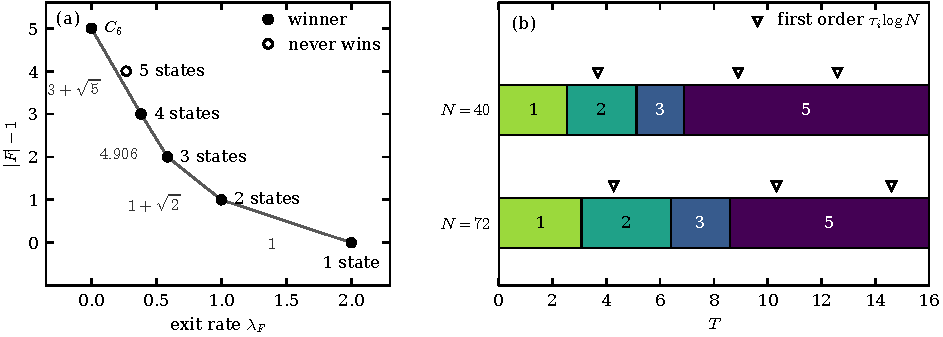
\includegraphics{fig_cycles}
\caption{(a) The points $(\lambda_F,\lvert F\rvert-1)$ of the arcs of the 6-cycle and of $C_6$,
with the lower-left boundary of their hull. The numbers beside the edges are the switch values
$\tau_i$ of Theorem~\ref{thm:hull}. The winners (filled) are the arcs of $1$ to $4$ states and
$C_6$, and the arc of $5$ states (open) never wins. (b) The support size of the exact mode on
$C_5$ with the uniform start, against $T$, at $N=40$ and $N=72$. The mode skips the arc of $4$
states. The triangles mark the first-order switch points $\tau_i\log N$ with $\tau_i=1$,
$1+\sqrt2$ and $2+\sqrt2$ (Table~\ref{tab:outcomes}).}
\label{fig:cycles}
\end{figure}

\section{The second-order theory}\label{sec:secondorder}

First order locates a crossing only up to a factor $1+o(1)$ in $T$. To locate
it up to $o(1)$ we need the constant in front of $N^{-(k-1)}e^{-T\lambda_F}$ for
every face that satisfies (H), together with the power of $T$. The plan is as
follows. Section~\ref{sec:tilt} defines the constant $K_F$.
Section~\ref{sec:locallaw} proves a local limit theorem inside a face and
deduces $M_F$ up to a factor $1+O(1/T+T^2/N)$. Section~\ref{sec:crossings}
compares 2 faces, Section~\ref{sec:papersAB} recovers Papers~A and~B, and
Section~\ref{sec:reducible} shows what can change without (H). In
this section gradients and Hessians in $\alpha$ are taken in the coordinates
$\alpha'=(\alpha_2,\dots,\alpha_k)$, $|\cdot|$ is the Euclidean norm, and
$q=(q_i)_{i\in F}$.

\subsection{The tilted chain and the constant}\label{sec:tilt}

To find the probability of a composition with fractions $\alpha$ we change the
rates so that $\alpha$ becomes typical. The optimal vector $r_\alpha$ in the
definition of $I_F(\alpha)$ gives a new generator $\widehat Q_\alpha$ on $F$, with
the same switching graph, whose stationary law is exactly $\alpha$. Under it the
visit fractions satisfy a central limit theorem with covariance
$\Gamma_\alpha/T$, and the price of the change of rates is $e^{-TI_F(\alpha)}$
times boundary factors for the start and the end of the path. The constant
$C_F(\alpha)$ collects these factors and the Gaussian normalization.

\begin{definition}[tilt and constants]\label{def:tilt}
Let $F$ be irreducible with $k\ge2$. For
$\alpha\in\Delta_F^\circ$ let $r_\alpha$ attain the supremum defining
$I_F(\alpha)$ (Proposition~\ref{prop:rate}(b)), and put
$\theta(\alpha)=A_Fr_\alpha/r_\alpha$ and $l_\alpha=\alpha/r_\alpha$
(entrywise). The \emph{tilted generator} is
$\widehat Q_\alpha=R^{-1}(A_F-\operatorname{diag}\theta(\alpha))R$ with
$R=\operatorname{diag}r_\alpha$. With $D=\operatorname{diag}\alpha$ let
\[
Z_\alpha=(\mathbf 1\alpha^\top-\widehat Q_\alpha)^{-1}-\mathbf 1\alpha^\top,
\qquad\Gamma_\alpha=DZ_\alpha+Z_\alpha^\top D,
\]
and let $\Sigma_\alpha$ be $\Gamma_\alpha$ with the row and column of state
$1$ deleted. Finally let $K_{\{i\}}=\mu_i$ for a single state, and
\[
C_F(\alpha)=\frac{(\mu\cdot r_\alpha)(l_\alpha\cdot\mathbf 1)}
{(2\pi)^{(k-1)/2}\sqrt{\det\Sigma_\alpha}},\qquad K_F=C_F(\alpha^*_F).
\]
\end{definition}

Nothing in Definition~\ref{def:tilt} changes when $r_\alpha$ is scaled. Note that
$l_\alpha\cdot r_\alpha=1$ and $I_F(\alpha)=\langle q-\theta(\alpha),\alpha\rangle$. Since
$r_\alpha$ minimizes $u\mapsto\sum_{i\ne j}\alpha_iq_{ij}u_j/u_i$, its derivative in $u_j$, which
is $\sum_il_{\alpha,i}q_{ij}-l_{\alpha,j}\theta_j(\alpha)$, vanishes at $r_\alpha$. Hence
\begin{equation}\label{eq:stationary}
l_\alpha^\top\bigl(A_F-\operatorname{diag}\theta(\alpha)\bigr)=0 .
\end{equation}
Also $(A_F-\operatorname{diag}\theta(\alpha))r_\alpha=0$ with $r_\alpha>0$, so $\theta(\alpha)\in
V_F$~\cite{bermanplemmons1994}. So $\widehat Q_\alpha$ is an irreducible generator with the
pattern of $A_F$ and, by~\eqref{eq:stationary}, stationary law $\alpha$. If
$(\mathbf 1\alpha^\top-\widehat Q_\alpha)v=0$, multiplying by $\alpha^\top$ gives $\alpha^\top
v=0$, so $\widehat Q_\alpha v=0$ and $v=0$. Thus $Z_\alpha$ exists, and
\begin{equation}\label{eq:Zprops}
Z_\alpha\mathbf 1=0,\qquad\alpha^\top Z_\alpha=0,\qquad
-\widehat Q_\alpha Z_\alpha=I-\mathbf 1\alpha^\top .
\end{equation}
So $\Gamma_\alpha\mathbf 1=0$. As $\Gamma_\alpha$ is symmetric, its adjugate is then a multiple of
$\mathbf 1\mathbf 1^\top$, so deleting another state instead of state $1$ gives the same
$\det\Sigma_\alpha$. At $\alpha^*_F$ the vector $u=r_F$ gives the value $\lambda_F=I_F(\alpha^*_F)$,
so $r_{\alpha^*_F}$ is a multiple of $r_F$, $\theta(\alpha^*_F)=q-\lambda_F\mathbf 1$, and
$l_{\alpha^*_F}$ is the matching multiple of $l_F$. In the local law below, $\mu\cdot r_\alpha$
accounts for the start of the path, $l_\alpha\cdot\mathbf 1$ for its free end, and $\Sigma_\alpha$
for the Gaussian spread of the occupation fractions.

For conductances $c_{ij}=c_{ji}$ on $F$ let
$\tree(c)=\sum_{\mathcal T}\prod_{\{i,j\}\in\mathcal T}c_{ij}$, the sum over
the spanning trees $\mathcal T$ of the complete graph on $F$.

\begin{proposition}[the constant]\label{prop:constant}
Let $F$ be irreducible with $k\ge2$.
\begin{enumerate}[(a)]
\item The maps $\alpha\mapsto\theta(\alpha)$, $I_F(\alpha)$, $\Sigma_\alpha$,
$r_\alpha$ and $l_\alpha$ (with $\sum_ir_{\alpha,i}=1$) are real-analytic on
$\Delta_F^\circ$, $\Sigma_\alpha$ is positive definite, and
$\nabla^2I_F(\alpha)=\Sigma_\alpha^{-1}$. Hence
$\det\Sigma_\alpha\cdot\det\nabla^2I_F(\alpha)=1$ and
$C_F(\alpha)=(\mu\cdot r_\alpha)(l_\alpha\cdot\mathbf 1)
\sqrt{\det\nabla^2I_F(\alpha)/(2\pi)^{k-1}}$.
\item Suppose that $\nu_iq_{ij}=\nu_jq_{ji}$ for $i,j\in F$ and some
$\nu\in(0,\infty)^F$. Then $r_\alpha$ is a multiple of $\sqrt{\alpha/\nu}$
and $l_\alpha$ of $\sqrt{\alpha\nu}$, and $\widehat Q_\alpha$ is reversible
with conductances $c_{ij}(\alpha)=\sqrt{\alpha_i\alpha_j}\,q_{ij}\sqrt{\nu_i/\nu_j}$.
Also $I_F(\alpha)=\sum_iq_i\alpha_i-\sum_{i\ne j}c_{ij}(\alpha)$, and
\[
\det\Sigma_\alpha=\frac{2^{k-1}(\prod_i\alpha_i)^2}{\tree(c(\alpha))},\qquad
C_F(\alpha)=\frac{(\mu\cdot r_\alpha)(l_\alpha\cdot\mathbf 1)}{(4\pi)^{(k-1)/2}}
\,\frac{\sqrt{\tree(c(\alpha))}}{\prod_i\alpha_i}.
\]
\end{enumerate}
\end{proposition}

\begin{proof}
The proof of (a) is in Appendix~\ref{app:torus} and uses Lemma~\ref{lem:perron}.

(b) Put $u=\sqrt{\alpha/\nu}$ and $l=\alpha/u=\sqrt{\alpha\nu}$. Then
$\sum_il_iq_{ij}=\sum_i\sqrt{\alpha_i\nu_i}\,q_{ij}$ and
$l_j(A_Fu)_j/u_j=\nu_j\sum_iq_{ji}\sqrt{\alpha_i/\nu_i}$ agree because $\nu_jq_{ji}=\nu_iq_{ij}$.
So $u$ is a critical point of $\sum_{i\ne j}\alpha_iq_{ij}u_j/u_i$, which is convex in $\log u$,
and $r_\alpha$ is a multiple of $u$. Then $\alpha_i(\widehat Q_\alpha)_{ij}=l_iq_{ij}u_j=
c_{ij}(\alpha)$, which is symmetric by reversibility, and $\alpha_i\theta_i(\alpha)=\sum_j
c_{ij}(\alpha)$ gives $I_F$.

For the determinant let $\mathcal L=-D\widehat Q_\alpha$, the Laplacian of the conductances. Fix
$\eta$ with $\eta_1=0$, and let $u=Z_\alpha\eta$ and $\zeta=D\eta-(\alpha\cdot\eta)\alpha$.
By~\eqref{eq:Zprops}, $\mathcal Lu=\zeta$ and $\alpha\cdot u=0$, so
$\eta^\top\Gamma_\alpha\eta=2(D\eta)^\top u=2\zeta^\top u$. Let $v=u-u_1\mathbf 1$. As
$\zeta\cdot\mathbf 1=0$ and $\mathcal L\mathbf 1=0$, we get $\zeta^\top u=\zeta^\top v$ and
$\mathcal Lv=\zeta$, and since $v_1=0$ the rows $2,\dots,k$ give $\mathcal L_{(1)}v'=\zeta'$. Here
$\mathcal L_{(1)}$ is $\mathcal L$ without row and column $1$, primes denote the coordinates
$2,\dots,k$, and $\zeta'=(D'-\alpha'\alpha'^\top)\eta'$ with $D'=\operatorname{diag}\alpha'$.
Hence $\Sigma_\alpha=2(D'-\alpha'\alpha'^\top)\mathcal L_{(1)}^{-1}(D'-\alpha'\alpha'^\top)$. The
matrix determinant lemma gives $\det(D'-\alpha'\alpha'^\top)=\prod_{i\ge2}\alpha_i\,
(1-\sum_{i\ge2}\alpha_i)=\prod_i\alpha_i$, and the matrix-tree theorem~\cite{bollobas1998} gives
$\det\mathcal L_{(1)}=\tree(c(\alpha))$.
\end{proof}

\begin{corollary}[symmetric faces]\label{cor:symface}
Let $F$ satisfy \textup{(H)} with $k\ge2$, and let $Q_F$ be symmetric with constant row sums.
Then $\lambda_F=q_i-\sum_{j\in F\setminus\{i\}}q_{ij}$ for every $i\in F$, $\alpha^*_F$ is uniform
on $F$, and
\[
K_F=\mu(F)\,k^{(k+1)/2}\sqrt{\tree(q_F)}\,(4\pi)^{-(k-1)/2},
\]
where $\tree(q_F)$ is $\tree(c)$ for the conductances $c_{ij}=q_{ij}$, $i,j\in F$.
\end{corollary}

\begin{proof}
The positive vector $\mathbf 1$ is a right and left eigenvector of $Q_F$, so it belongs to the
Perron root. So $\lambda_F$ is minus the row sum, $r_F$ and $l_F$ are multiples of $\mathbf 1$, and
$\alpha^*_F=\mathbf 1/k$.
At $\alpha=\mathbf 1/k$, Proposition~\ref{prop:constant}(b) with $\nu=\mathbf 1$ gives
$r_\alpha=\mathbf 1$, $l_\alpha=\alpha$ and $(\mu\cdot r_\alpha)(l_\alpha\cdot\mathbf 1)=\mu(F)$.
Also $c_{ij}(\alpha)=q_{ij}/k$, so $\tree(c(\alpha))=k^{-(k-1)}\tree(q_F)$, and
$\prod_i\alpha_i=k^{-k}$.
\end{proof}

\subsection{The local law and the face maxima}\label{sec:locallaw}

Inside the face the occupation fractions fluctuate on the scale $T^{-1/2}$ in $k-1$ directions. So
a single composition gets the factor $T^{(k-1)/2}$ times the volume $N^{-(k-1)}$ of a lattice cell.

\begin{theorem}[local law]\label{thm:local}
Let $F$ satisfy (H) with $k\ge2$, and let $\mathcal K\subset\Delta_F^\circ$ be
compact. Uniformly for $\alpha\in\mathcal K$ and $T\ge1$,
\[
f_T(\alpha)=T^{(k-1)/2}C_F(\alpha)e^{-TI_F(\alpha)}\bigl(1+O_{\mathcal K}(1/T)\bigr).
\]
For $F=\{i\}$, $f_T=\mu_ie^{-q_iT}$.
\end{theorem}

In words, the density of the visit fractions on the event that the chain stays
in $F$ is a Gaussian factor $T^{(k-1)/2}$ times the large-deviation factor
$e^{-TI_F(\alpha)}$ times the constant $C_F(\alpha)$, with a relative error
$O(1/T)$ that is uniform away from the boundary of the face.

\emph{Idea of the proof.} The proof is in Appendix~\ref{app:torus}. The sum
over words that defines $H$ is a matrix resolvent, so Cauchy's formula writes $H$
as an integral over a torus of radii $\theta(\alpha)$ (Lemma~\ref{lem:torus}).
All the coefficients are nonnegative, so the integrand is largest at the real
point, and a Laplace lemma with a parameter (Lemma~\ref{lem:laplace}) gives the
expansion. The Hessian at the real point is computed from the Perron root of a
perturbed generator (Lemma~\ref{lem:perron}), and this is where $\Sigma_\alpha$
comes from. The hypothesis $\mu(F)>0$ is needed, since $f_T=C_F=0$ when
$\mu(F)=0$. Also $f_T(\alpha)$ is continuous and positive in $(T,\alpha)$, as
$H$ is a convergent power series with some $W(m)>0$ by (H).

\begin{lemma}[discrete and continuum]\label{lem:discrete}
Let $F$ satisfy (H) with $k\ge2$, and let $\mathcal K\subset\Delta_F^\circ$ be
compact. Uniformly for $\operatorname{supp}n=F$ with $n/N\in\mathcal K$ and
$1\le T\le N^{1/2}$,
$P_N(n)=N^{-(k-1)}f_T(n/N)(1+O_{\mathcal K}(T^2/N))$.
\end{lemma}

The proof is in Appendix~\ref{app:torus}. With Theorem~\ref{thm:local} it sharpens the error in
Theorem~\ref{thm:first}(i) to $\frac{k-1}2\log T+\log C_F(n/N)+O(1/T+T^2/N)$.

\begin{theorem}[face maxima]\label{thm:facemax}
Let $F$ satisfy (H). If $k\ge2$, then uniformly for $1\le T\le N^{1/3}$,
\[
M_F=N^{-(k-1)}T^{(k-1)/2}K_Fe^{-T\lambda_F}\bigl(1+O(1/T+T^2/N)\bigr),
\]
and every maximizer $\hat n$ satisfies $\hat n/N=\alpha^*_F+O(1/T)$. For $k=1$,
$M_{\{i\}}$ is given by~\eqref{eq:vertexmax}. In both cases,
uniformly for $1\le T\le N^{1/3}$,
\begin{equation}\label{eq:logmax}
\log M_F=-(k-1)L+\tfrac{k-1}2\log T+\log K_F-T\lambda_F+O(1/T+T^2/N).
\end{equation}
\end{theorem}

In words, the best composition on $F$ sits within $O(N/T)$ of $N\alpha^*_F$,
and its probability is the Gaussian peak of the local law at $\alpha^*_F$. The
factor $N^{-(k-1)}$ is the volume of a lattice cell, and $T^{(k-1)/2}$ is the
height of a Gaussian density whose spread in each free direction is of order
$T^{-1/2}$.

\emph{Idea of the proof.} Near $\alpha^*_F$ we use the local law and
Lemma~\ref{lem:discrete}, and maximize a Gaussian with a small linear
perturbation. Away from $\alpha^*_F$ the rate exceeds $\lambda_F$ by a fixed
amount, and Lemma~\ref{lem:upper}, applied with finitely many vectors $\theta$,
shows that these compositions are exponentially less likely in $T$. For bounded
$T$ positivity and continuity suffice.

\begin{proof}
For $k=1$ this is~\eqref{eq:vertexmax}. Let $k\ge2$, put
$X=N^{-(k-1)}T^{(k-1)/2}K_Fe^{-T\lambda_F}$ and $x=\alpha'-\alpha^{*\prime}_F$. By
Propositions~\ref{prop:rate}(a) and~\ref{prop:constant}(a), $I_F$ and $\log C_F$ are
real-analytic near $\alpha^*_F$, $I_F$ has its minimum $\lambda_F$ there and $\nabla^2I_F>0$. So
there is a closed ball $U=\{|x|\le\rho_0\}\subset\Delta_F^\circ$ on which
$c_U|x|^2\le I_F-\lambda_F\le C_U|x|^2$, $|\log(C_F/K_F)-\gamma\cdot x|\le C_1|x|^2$ with
$\gamma=\nabla\log C_F(\alpha^*_F)$, and $\log C_F$ is $C_3$-Lipschitz.

\emph{Outside $U$.} As $I_F$ is lower semicontinuous, Proposition~\ref{prop:rate}(a) gives
$I_F\ge\lambda_F+3\eta$ on $\Delta_F\setminus U^\circ$ for some $\eta>0$. Since
$I_F(\beta)=\sup_{u>0}\langle q-A_Fu/u,\beta\rangle$ and $A_Fu/u\in V_F$, compactness gives
finitely many $\theta_j\in V_F$ with $\max_j\langle q-\theta_j,\beta\rangle>\lambda_F+2\eta$ on
$\Delta_F\setminus U^\circ$.
Lemma~\ref{lem:upper} then gives
$P_N(n)\le C(T/N)^{k-1}e^{-T(\lambda_F+2\eta)}=X\cdot O(T^{(k-1)/2}e^{-2\eta T})$ for
$\supp n=F$ and $n/N\notin U^\circ$.

\emph{Inside $U$.} By Theorem~\ref{thm:local} and Lemma~\ref{lem:discrete} with $\mathcal K=U$,
for $\alpha=n/N\in U$,
\begin{equation}\label{eq:insideU}
P_N(n)=X\,\tfrac{C_F(\alpha)}{K_F}\,e^{-T(I_F(\alpha)-\lambda_F)}(1+E),
\qquad|E|\le C_2(1/T+T^2/N).
\end{equation}
For $T\ge2C_1/c_U$ the middle factors are at most
$\exp(\sup_x[\gamma\cdot x-\frac{c_UT}2|x|^2])=e^{|\gamma|^2/(2c_UT)}$, so
$M_F\le X(1+O(1/T+T^2/N))$. For the lower bound let $n^0$ have support $F$ and
$|n^0_i-N\alpha^*_{F,i}|<1$ for all $i$, which exists for $N\ge N_0$ since
every $\alpha^*_{F,i}>0$. Then $C_F(n^0/N)\ge K_Fe^{-kC_3/N}$ and
$T(I_F(n^0/N)-\lambda_F)\le C_Uk^2T/N^2$, so~\eqref{eq:insideU} gives
$P_N(n^0)\ge X(1-O(1/T+T^2/N))$. Fix $T_2$ so large that the 2 bounds above give
$M_F/X\in[\frac12,\frac32]$ for $T\ge T_2$. For $1\le T\le T_2$, $f_T$ is positive and continuous
on $[1,T_2]\times U$, so Lemma~\ref{lem:discrete} gives $M_F/X\in[c,C]$. This gives the first
display and~\eqref{eq:logmax}.

\emph{The maximizer.} For $T\ge T_3$ with $T_3$ large, the bound outside $U$ is below $X/2\le
P_N(n^0)$, so $\hat\alpha=\hat n/N\in U$ and $|E|\le\frac12$. Taking logarithms in $P_N(\hat
n)\ge P_N(n^0)$ gives $c_UT|\hat x|^2\le C_3|\hat x|+C_4(1/T+T^2/N)\le C_3|\hat x|+2C_4/T$ with
$\hat x=\hat\alpha'-\alpha^{*\prime}_F$, because $T\le N^{1/3}$ gives $T^2/N\le1/T$. This step uses
the exponent $\frac13$, and it gives $|\hat x|=O(1/T)$. For $1\le T<T_3$ the claim holds since
$|\hat x|$ is bounded.
\end{proof}

\subsection{Crossings and tie windows}\label{sec:crossings}

We now compare 2 faces. Taking logarithms in Theorem~\ref{thm:facemax}, the
difference $\log M_F-\log M_G$ is an explicit increasing function of $T$ up to
$O(1/T+T^2/N)$, and its zero is the crossing.

\begin{theorem}[the crossing equation]\label{thm:crossing}
Let $F$ and $G$ satisfy (H), with $\Delta=k_F-k_G\ge1$ and
$\delta=\lambda_G-\lambda_F>0$, and let $D_N(T)=\log M_F-\log M_G$.
\begin{enumerate}[(i)]
\item For large $N$, $D_N$ has a zero in
$[\frac{\Delta}{2\delta}L,\frac{2\Delta}{\delta}L]$.
\item For large $N$, every zero $T_N\in[1,N^{1/3}]$ of $D_N$ satisfies
\begin{equation}\label{eq:crossing}
\delta T_N+\frac\Delta2\log T_N=\Delta L-\log\frac{K_F}{K_G}
+O\Bigl(\frac1L\Bigr).
\end{equation}
\item All such zeros lie in one interval of length $O(1/L)$, and
\[
T_N=\frac\Delta\delta\Bigl[L-\frac12\log L+b_{FG}\Bigr]
+O\Bigl(\frac{\log L}L\Bigr),\qquad
b_{FG}=-\frac12\log\frac\Delta\delta-\frac1\Delta\log\frac{K_F}{K_G}.
\]
\end{enumerate}
\end{theorem}

\begin{proof}
By~\eqref{eq:logmax}, uniformly on $[1,N^{1/3}]$,
$D_N(T)=-\Delta L+\frac\Delta2\log T+\delta T+\log\frac{K_F}{K_G}+O(1/T+T^2/N)$.

(i) At $T=\frac{\Delta}{2\delta}L$ this is $-\frac\Delta2L+O(\log L)<0$, and at
$T=\frac{2\Delta}\delta L$ it is $\Delta L+O(\log L)>0$. For fixed $N$, $M_F$ is a maximum of
finitely many polynomials in $h$, and it is positive because $F$ is admissible. So $D_N$ is
continuous and has a zero in between.

(ii) Let $\psi(T)=\delta T+\frac\Delta2\log T$, which is increasing. At a zero
$T_N\in[1,N^{1/3}]$, $\psi(T_N)=\Delta L-\log(K_F/K_G)+O(1)$. This is larger than
$\psi(\frac\Delta{2\delta}L)=\frac\Delta2L+O(\log L)$, and $\delta T_N\le\psi(T_N)$. So
$\frac\Delta{2\delta}L<T_N\le\frac{2\Delta}\delta L$, and then $O(1/T_N+T_N^2/N)=O(1/L)$.

(iii) Let $\psi(T^\circ)=\Delta L-\log(K_F/K_G)$. As $\psi'\ge\delta$, every zero is within
$O(1/L)$ of $T^\circ$. Also $T^\circ=\frac\Delta\delta L+O(\log L)$, so
$\log T^\circ=\log L+\log\frac\Delta\delta+O(\log L/L)$, which gives the explicit form.
\end{proof}

In words: the larger face $F$ pays $N^{-\Delta}$ for spreading and gains
$e^{\delta T}$ for staying, and its Gaussian peak gives an extra factor
$T^{\Delta/2}$; the crossing balances the 3. The explicit form in (iii)
converges slowly, so computations should solve~\eqref{eq:crossing} (see
Corollary~\ref{cor:C4}). We do not prove that the zero of $D_N$ is unique in
general.

Sometimes several faces tie at first order: at some $\tau^*$ more than 2 faces
minimize $\Phi_{\tau^*}$, as all faces do for the model of Paper~B. Then the
competition plays out in a window $T=\tau^*(L-\frac12\log L+t)$ with $t$ of
order $1$. In this window each tied face has a line $\ell_F(t)$, and the mode
follows the highest line.

\begin{theorem}[tie windows]\label{thm:window}
Fix $\tau^*>0$. Let $m^*$ be the least value of $\Phi_{\tau^*}$ over the
admissible faces and $\mathcal F^*$ the set of minimizers. Assume that every
face in $\mathcal F^*$ is irreducible. By Theorem~\ref{thm:hull}(c) this holds
if $Q$ has symmetric support or $\mu$ has full support. Put $T=\tau^*(L-\frac12\log L+t)$, and for
$F\in\mathcal F^*$ let
$\ell_F(t)=\log K_F+\frac{k_F-1}2\log\tau^*-\tau^*\lambda_Ft$ and
$E(t)=\max_{G\in\mathcal F^*}\ell_G(t)$.
\begin{enumerate}[(i)]
\item Uniformly for $t$ in compact sets, for $F\in\mathcal F^*$,
$\log M_F=-m^*L+\frac{m^*}2\log L+\ell_F(t)+O(\log L/L)$.
\item There are $\varepsilon_1,\varepsilon_0>0$ such that for large $N$ and
$|T/L-\tau^*|\le\varepsilon_1$, every admissible $F\notin\mathcal F^*$ has
$M_F\le N^{-\varepsilon_0}\max_{G\in\mathcal F^*}M_G$.
\item There are $\varepsilon,t_0>0$ such that for large $N$ and
$t_0\le|t|\le\varepsilon L$, every global mode lies on a face
$F\in\mathcal F^*$ with $\ell_F=E$ on $[t_0,\infty)$ if $t>0$, or on
$(-\infty,-t_0]$ if $t<0$. Such a face has the least $\lambda_F$ in
$\mathcal F^*$ if $t>0$ and the largest if $t<0$.
\end{enumerate}
Consequently, for every $\eta>0$ and large $N$, if $|t|\le\varepsilon L$ is at
distance at least $\eta$ from every kink of $E$, then every global mode lies
on a face whose line equals $E$ near $t$. So the line of the face that
carries the global mode changes only at
$T=\tau^*(L-\frac12\log L+t_j)+o(1)$, where $t_j$ runs over the kinks of $E$,
and it changes near each kink. Faces with identical lines (the same $k_F$,
$\lambda_F$ and $K_F$) tie at this order and give no crossing.
\end{theorem}

In words: inside the window the logarithm of every tied face maximum is the
same leading term plus the line $\ell_F(t)$, faces that do not tie are smaller by
a power of $N$, and far out in the window the face with the least (for $t>0$) or
largest (for $t<0$) exit rate wins.

\begin{proof}
Every $F\in\mathcal F^*$ is admissible and irreducible, so it satisfies (H) by
Lemma~\ref{lem:admissible}(b). Write $T=\tau^*L(1+y)$ with $y=(t-\frac12\log L)/L$, so that
$|y|\le\frac12$ for $|t|\le L/4$ and large $N$. By~\eqref{eq:logmax} and
$\tau^*\lambda_F+k_F-1=m^*$, uniformly for $|t|\le L/4$,
\begin{equation}\label{eq:windowline}
\log M_F=-m^*L+\tfrac{m^*}2\log L+\ell_F(t)+\tfrac{k_F-1}2\log(1+y)+O(1/L)
\qquad(F\in\mathcal F^*).
\end{equation}
For $t$ in a compact set, $\log(1+y)=O(\log L/L)$, which gives (i).

(ii) Let $g>0$ be the least value of $\Phi_{\tau^*}(F)-m^*$ over the admissible
$F\notin\mathcal F^*$. As $0\le\lambda_F\le q_{\max}$, for
$|\tau-\tau^*|\le\varepsilon_1=g/(4q_{\max}+4)$ we have $\Phi_\tau(F)-\Phi_\tau(G)\ge g/2$ for
such $F$ and all $G\in\mathcal F^*$. With $\tau=T/L$, Theorem~\ref{thm:first}(ii) gives
$\log M_F-\log M_G\le-\frac g2L+O(\log L)\le-\frac g4L$.

(iii) Take $t_0\ge1$ larger than every $|t_j|$ and $\varepsilon\le\min(\frac14,\varepsilon_1/(2\tau^*))$,
so that (ii) applies. Let $t\ge t_0$, let $\ell_F=E$ on $[t_0,\infty)$, and let $G\in\mathcal F^*$
with $\ell_G\ne\ell_F$, so that $\lambda_F\le\lambda_G$. As both faces are tied,
$\Delta=k_F-k_G=\tau^*(\lambda_G-\lambda_F)\ge0$. If $\Delta=0$, \eqref{eq:windowline} gives
$\log(M_F/M_G)=\log(K_F/K_G)+O(1/L)$ with $K_F>K_G$. If $\Delta>0$,
$\log(M_F/M_G)=\Delta t+\ell_F(0)-\ell_G(0)+\frac\Delta2\log(1+y)+O(1/L)$, where
$|\log(1+y)|\le2|y|\le t/2$ for large $N$, so it is positive if $t_0$ is large. The case $t\le-t_0$ is the same.

For the consequence, fix $\eta>0$ and let $S_\eta=[-t_0,t_0]\setminus\bigcup_j(t_j-\eta,t_j+\eta)$.
For $G\in\mathcal F^*$, $E-\ell_G$ is convex, piecewise linear and nonnegative with kinks only at
kinks of $E$. So its zero set is empty, a single kink of $E$, or an interval whose finite endpoints
are kinks of $E$, and on each component of $S_\eta$ either $\ell_G=E$ or $E-\ell_G\ge g_\eta>0$.
Then (i) and (ii) give the claim on $S_\eta$, and (iii) for $t_0\le|t|\le\varepsilon L$.
\end{proof}

\subsection{Papers A and B}\label{sec:papersAB}

We use the polynomials $S_{a,b}$ and $S_N$, the root $u_N$, the crossing $p_N$,
$z_N=N(1-p_N)$ and $c_0=\frac12\log(\pi/8)$ of Section~\ref{sec:notation}. The
first result shows that a single state against a symmetric pair is Kagey's
board at every $N$.

\begin{proposition}[an exact pair identity]\label{prop:pair}
Let $i\ne j$ with $q_{ij}=q_{ji}=a$, $q_i=q_j=q$ and $\mu_i=\mu_j>0$, and let
$F=\{i,j\}$. For every $N\ge2$, $1\le m\le N-1$ and $h>0$ such that $I+hQ$ is
stochastic and $qh<1$,
\[
\frac{P_N(me_i+(N-m)e_j)}{P_N(Ne_i)}=S_{m,N-m}(u),\qquad u=\frac{ah}{1-qh}.
\]
So the balanced compositions, with $m=\lfloor N/2\rfloor$ or
$m=\lceil N/2\rceil$, are the most likely ones with support $F$,
$M_F=M_{\{i\}}S_N(u)$, and $M_F>M_{\{i\}}$ exactly when $u>u_N$.
\end{proposition}

\begin{proof}
A path with this composition is a word in $i,j$ with $m$ letters $i$. Each stay has probability
$1-qh$ and each switch $ah$, so a word with $s$ switches has probability
$\mu_i(1-qh)^{N-1-s}(ah)^s=\mu_i(1-qh)^{N-1}u^s$, while $P_N(Ne_i)=\mu_i(1-qh)^{N-1}$. Sum over
the words. The bin polynomials of~\cite{paperA} grow coefficientwise as the bin moves toward the
middle, and $S_{m,N-m}=S_{N-m,m}$. So the balanced $m$ give the largest $S_{m,N-m}(u)$. Finally
$S_N$ increases strictly and equals $1$ only at $u_N$ (Section~\ref{sec:notation}).
\end{proof}

The identity in Proposition~\ref{prop:pair} is checked in Lean.

\begin{corollary}[Paper A]\label{cor:paperA}
Let $d=2$, $q_{12}=q_{21}=1$ and $\mu=(\frac12,\frac12)$, the walk of~\cite{paperA} with
$T=N(1-p)$. Then $K_{\{1\}}=K_{\{2\}}=\frac12$ and $K_{\{1,2\}}=\sqrt{2/\pi}$, so
$b_{FG}=c_0$ for $F=\{1,2\}$ and $G=\{1\}$. For every $N\ge2$, $M_{\{1,2\}}=M_{\{1\}}$ holds
exactly at $T=z_N$, and $z_N+\frac12\log z_N=L+c_0+O(1/L)$.
\end{corollary}

\begin{proof}
Corollary~\ref{cor:symface} with $k=2$, $\tree(q_F)=1$ and $\mu(F)=1$ gives $K_{\{1,2\}}$, and
then $b_{FG}=-\log(K_{\{1,2\}}/K_{\{1\}})=c_0$. Proposition~\ref{prop:pair} with $a=q=1$ gives
$M_{\{1,2\}}=M_{\{1\}}S_N(h/(1-h))$, and $h/(1-h)=u_N$ exactly when $p=p_N$. So for every $N$
the only zero of $D_N$ is $z_N$, and by Theorem~\ref{thm:crossing}(i) it lies in
$[L/2,2L]\subset[1,N^{1/3}]$ for large $N$. Then Theorem~\ref{thm:crossing}(ii) with
$\Delta=\delta=1$ gives the equation.
\end{proof}

This is the crossing equation of~\cite{paperA} without its terms $1/(8z_N)$ and $R_N$. The term
$1/(8z_N)$ is $(c_{\{1\}}-c_{\{1,2\}})/z_N$ in the notation of Remark~\ref{rem:nextterm}, whose
proof we omit, with $c_{\{1\}}=0$ and $c_{\{1,2\}}=-\frac18$.

\begin{corollary}[Paper B]\label{cor:paperB}
Let $Q=J-dI$, where $J$ is the all-ones matrix, and let $\mu$ be uniform, the model
of~\cite{paperB}. A face of $k$ states has $\lambda_F=d-k$, $\alpha^*_F$ uniform and
$K_F=\frac1dk^{k+1/2}(4\pi)^{-(k-1)/2}$. So $\Phi_1(F)=d-1$ for every face, and all faces tie at
$\tau=1$. The crossing of a face of $k\ge2$ states with a vertex has $\Delta=\delta=k-1$ and
$b_{FG}=a_k=\frac12\log(4\pi)-\frac{k+1/2}{k-1}\log k$, the constant of the vertex crossing
of~\cite{paperB}.
\end{corollary}

\begin{proof}
Each $Q_F$ is symmetric with row sums $-(d-k)$, and the complete graph on $F$ has $k^{k-2}$
spanning trees by Cayley's formula. So Corollary~\ref{cor:symface} with $\mu(F)=k/d$ gives
$\lambda_F$, $\alpha^*_F$ and $K_F$. A vertex has $K=\frac1d$ and $\lambda=d-1$, so
$b_{FG}=-\frac1{k-1}\log(dK_F)=a_k$. The arithmetic that gives $b_{FG}$ from $K_F$ here and in
Corollary~\ref{cor:paperA} is checked in Lean. At $\tau^*=1$, Theorem~\ref{thm:window} describes
the tie window, and~\cite{paperB} resolves this window in full.
\end{proof}

\subsection{Reducible faces}\label{sec:reducible}

\begin{remark}[scope of the $\frac12$]\label{rem:half}
The coefficient $\frac12$ of $\log\log N$ in Theorems~\ref{thm:crossing} and~\ref{thm:window} is
due to the power $T^{(k-1)/2}$ in Theorem~\ref{thm:facemax}, so it needs only (H). At a kink of
$E$ where the line of $G$ gives way to that of $F$ as $t$ increases, $\Delta=\tau^*\delta$ and
$t_j=b_{FG}$. So every change in a tie window is a crossing of Theorem~\ref{thm:crossing}. The
best composition of a reducible face can visit a state only once,
with no Gaussian window in that direction. Then the $\frac12$ can fail, and in the next example it
is $1$ and then $0$.
\end{remark}

\begin{proposition}[a directed $3$-cycle]\label{prop:threecycle}
Let $d=3$, $q_{12}=b>2$, $q_{23}=q_{31}=1$, all other rates $0$, and
$\mu_1=1$.
\begin{enumerate}[(i)]
\item The admissible faces are $\{1\}$, $\{1,2\}$ (reducible, $\lambda=1$) and
$\{1,2,3\}$ (irreducible, $\lambda=0$). Exactly
$M_{\{1\}}=(1-bh)^{N-1}$ and $M_{\{1,2\}}=bh(1-h)^{N-2}$, and the latter is
attained only at $n=(1,N-1,0)$. For the full face,
$\alpha^*=(1,b,b)/(1+2b)$, $\det\nabla^2I=(1+2b)^4/(3b^2)$ and
$K_{\{1,2,3\}}=(1+2b)^2/(2\sqrt3\,\pi b)$.
\item $M_{\{1\}}=M_{\{1,2\}}$ has exactly one root $T^{(1)}_N$ with $bh<1$. It
satisfies $(b-1)T+\log T=L-\log b+O(T^2/N)$, so
$T^{(1)}_N=\frac1{b-1}[L-\log L+\log\frac{b-1}b]+O(\log L/L)$, and the
coefficient of $\log\log N$ in the bracket is $1$.
\item Every root $T\in[L/2,2L]$ of $M_{\{1,2\}}=M_{\{1,2,3\}}$ satisfies
$T=L+\log\frac{2\sqrt3\,\pi b^2}{(1+2b)^2}+O(1/L)$, so the coefficient of
$\log\log N$ is $0$. These roots lie in an interval of length $O(1/L)$.
\item Both are changes of the global mode. For large $N$ and $T\le N^{1/3}$,
the mode is $(N,0,0)$ for $T<T^{(1)}_N$, it is $(1,N-1,0)$ between
$T^{(1)}_N$ and the smallest root in (iii), and it lies on the full face above
the largest root in (iii).
\end{enumerate}
\end{proposition}

In words: the face $\{1,2\}$ is reducible, and its best composition
$(1,N-1,0)$ visits state $1$ once and then stays in state $2$. Its maximum is
about $b(T/N)e^{-T}$, with the power $T^1$ where an irreducible pair would have
$T^{1/2}$. This changes the coefficient of $\log\log N$ at both crossings.

\begin{proof}
(i) The chain moves only along $1\to2\to3\to1$ from $1$, which gives the supports and the
components $\{1\}$, $\{2\}$ of $\{1,2\}$. A path with support
$\{1,2\}$ is $1^{n_1}2^{n_2}$, of probability $(1-bh)^{n_1-1}bh(1-h)^{n_2-1}$, and raising $n_1$
by one multiplies it by $(1-bh)/(1-h)<1$. For the full face $\lambda=0$, $r=\mathbf 1$, and
$l=\alpha^*=(1,b,b)/(1+2b)$ is the stationary law, so $(\mu\cdot r)(l\cdot\mathbf 1)=1$. The
ratios $u_2/u_1$, $u_3/u_2$ and $u_1/u_3$ have product $1$, so the AM--GM inequality gives
$I(\alpha)=\sum_iq_i\alpha_i-3(b\alpha_1\alpha_2\alpha_3)^{1/3}$. Let
$g=(\alpha_1\alpha_2\alpha_3)^{1/3}$, $w=1/\alpha$ and $s=1+2b$. The Hessian of $g$ in all 3
coordinates is $-gM$ with $M=\frac13\operatorname{diag}(w)^2-\frac19ww^\top$, so
$\nabla^2I=3b^{1/3}g\,J^\top MJ$, where $J$ is the Jacobian of
$(\alpha_2,\alpha_3)\mapsto(1-\alpha_2-\alpha_3,\alpha_2,\alpha_3)$. At $\alpha^*$,
$3b^{1/3}g=3b/s$ and $w=s(1,y,y)$ with $y=1/b$. So $J^\top MJ$ has diagonal entries
$\frac29s^2(1+y+y^2)$ and off-diagonal entries $\frac19s^2(2+2y-y^2)$, and
$\det J^\top MJ=\frac{s^4}{81}\cdot3y^2(2+y)^2=\frac{s^6}{27b^4}$. Hence
$\det\nabla^2I=s^4/(3b^2)$, and Proposition~\ref{prop:constant}(a) gives $K_{\{1,2,3\}}$. The
exact parts of (i) are checked in Lean.

(ii) Let $D_1=\log M_{\{1,2\}}-\log M_{\{1\}}=\log(bh)+(N-2)\log(1-h)-(N-1)\log(1-bh)$. Then
$D_1'(h)=\frac1h-\frac{N-2}{1-h}+\frac{b(N-1)}{1-bh}>0$ for $bh<1$, while $D_1\to-\infty$ as
$h\to0$ and $D_1\to\infty$ as $bh\to1$. So there is exactly one root (this is checked in
Lean). Expanding, $D_1=\log b+\log T-L+(b-1)T+O(T^2/N)$, which is positive at $T=L/(b-1)$ and
negative at $T=L/(2(b-1))$. So the root lies between them, and $\log T=\log L-\log(b-1)+O(\log
L/L)$ gives the expansion.

(iii) Here $\log M_{\{1,2\}}=\log b+\log T-L-T+O(T^2/N)$, and Theorem~\ref{thm:facemax} for the
full face ($k=3$, $\lambda=0$, $\mu(F)=1$) gives $\log M_{\{1,2,3\}}=-2L+\log T+\log
K_{\{1,2,3\}}+O(1/T+T^2/N)$. So on $[L/2,2L]$
the difference is $L-T+\log b-\log K_{\{1,2,3\}}+O(1/L)$, which gives (iii).

(iv) Lemma~\ref{lem:upper} with $\theta=q$ gives $M_{\{1,2,3\}}\le C(T/N)^2$. For $T<T^{(1)}_N$,
$M_{\{1\}}>M_{\{1,2\}}$ by (ii), and $M_{\{1\}}\ge N^{-b/(b-1)-o(1)}$ since $T^{(1)}_N\le
L/(b-1)$. This beats $C(T/N)^2$ because $b/(b-1)<2$. For $T>T^{(1)}_N$,
$M_{\{1,2\}}>M_{\{1\}}$. For $T\le L/2$, $\log M_{\{1,2\}}-\log M_{\{1,2,3\}}\ge L-T-\log T-C>0$.
On $[L/2,2L]$ the sign is that of the formula in (iii), which is positive at $L/2$ and negative at
$2L$. For $2L\le T\le N^{1/3}$ the same formula is at most $-L+C<0$.
\end{proof}

\begin{remark}[the next term, proof omitted]\label{rem:nextterm}
Carrying the Laplace argument behind Theorem~\ref{thm:local} one term further gives the factor
$1+c(\alpha)/T+O(T^{-3/2})$ there. Here $c(\alpha)$ is the coefficient of $1/T$ in the next step
of Lemma~\ref{lem:laplace} for the integral~\eqref{eq:A-fT}, divided by $\chi(\alpha,0)$. It is a
Gaussian moment of the $\varphi$-derivatives of $\Psi$ of orders $3$ and $4$ and of $\chi$ of
orders $1$ and $2$ at $\varphi=0$. Then~\eqref{eq:logmax} gains the term $c_F/T$, with
$c_F=c(\alpha^*_F)+\frac12\gamma^\top\Sigma_{\alpha^*_F}\gamma$ and
$\gamma=\nabla\log C_F(\alpha^*_F)$, and the error becomes $O(T^{-3/2}+T^2/N)$. So at every
crossing
\[
T_N\Bigl(\Delta L-\frac\Delta2\log T_N-\delta T_N-\log\frac{K_F}{K_G}\Bigr)
=c_F-c_G+O\bigl(T_N^{-1/2}+T_N^3/N\bigr).
\]
Here $c_{\{i\}}=0$. Comparing with the terms of order $1/z$ in the expansions of~\cite{paperA}
and~\cite{paperB} gives $c_F=-1/(8q_{ij})$ for a pair with $q_{ij}=q_{ji}$, $q_i=q_j$ and
$\mu_i=\mu_j$, and $c_F=-(k-1)/8$ for a face of $k$ states when $Q=J-dI$ and $\mu$ is constant on
$F$. We omit the details.
\end{remark}

\section{The 4-cycle and other graphs}\label{sec:examples}

In this section $Q$ is symmetric. So the admissible faces are the connected
faces with positive start mass, and they satisfy (H)
(Lemma~\ref{lem:admissible}). By Theorem~\ref{thm:hull}(c),
Theorem~\ref{thm:window} applies at every tie. We call the faces in
$\mathcal F_\tau$ the \emph{winners} at $\tau$. We first complete the worked
example of Section~\ref{sec:worked} with all its constants, then show on $K_3$
that the start can decide the winner, and then list the outcomes for other
graphs.

\begin{corollary}[the 4-cycle cascade]\label{cor:C4}
Let $Q$ be the 4-cycle $C_4$ with $q_{i,i\pm1}=1$ (indices mod $4$), and let
$\mu$ be uniform.
\begin{enumerate}[(a)]
\item The admissible faces are the vertices, the adjacent pairs, the arcs of
three states and $C_4$, with exit rates $2$, $1$, $2-\sqrt2$ and $0$. The
winners are the vertices for $\tau<1$, the adjacent pairs for $1<\tau<2$ and
$C_4$ for $\tau>2$. The arcs of three states never win.
\item $K_{\rm vertex}=\frac14$, $K_{\rm pair}=1/\sqrt{2\pi}$,
$K_{\rm arc3}=(4+3\sqrt2)/(4\pi)$ and $K_{C_4}=8/\pi^{3/2}$, and
$\det\Sigma=1/512$ on $C_4$.
\item For every $N\ge2$ and $0<h<\frac12$, $M_{\rm pair}=M_{\rm vertex}S_N(u)$
with $u=h/(1-2h)$. So the face maxima of a vertex and an adjacent pair cross
exactly at $u=u_N$, the crossing of~\cite{paperA}. For large $N$ this
crossing satisfies $T+\frac12\log T=L+c_0+O(1/L)$.
\item For large $N$, every crossing $T_N\in[1,N^{1/3}]$ of the face maxima of
an adjacent pair and $C_4$ satisfies $T_N+\log T_N=2L-\log(8\sqrt2/\pi)+O(1/L)$.
\item Put $b=-\frac12\log2-\frac12\log(8\sqrt2/\pi)$. In the tie window at
$\tau=1$ the face that carries the global mode changes from the vertices to
the adjacent pairs only at $T=L-\frac12\log L+c_0+o(1)$. In the tie window at
$\tau=2$ it changes from the adjacent pairs to $C_4$ only at
$T=2(L-\frac12\log L+b)+o(1)$.
\end{enumerate}
\end{corollary}

In words, the mode moves from a vertex to an adjacent pair at the crossing of
Kagey's board, exactly at every $N$, and from the pairs to the whole cycle at a
crossing whose equation has the coefficient $1=\frac\Delta2$ of $\log T$, since
the cycle has two more states than a pair.

\begin{proof}
(a) A proper face that is not an arc is disconnected, so it is not
admissible. For an adjacent pair $-Q_F$ has rows $(2,-1)$ and $(-1,2)$, with
least eigenvalue $1$. For an arc of three states $-Q_F=2I-A$, where $A$ is the
adjacency matrix of the path on three states, and $r=(1/\sqrt2,1,1/\sqrt2)$ is a
positive eigenvector with eigenvalue $2-\sqrt2$. Also $Q\ones=0$. So
$\Phi_\tau$ equals $2\tau$, $\tau+1$, $(2-\sqrt2)\tau+2$ and $3$, and comparing
the first, second and fourth gives the winners. Since $2-\sqrt2>\frac12$, the
3-arc has $\Phi_\tau>\frac12(\tau+1)+\frac12\cdot3$, which is at least the
smaller of the exponents of the pair and of $C_4$. So it never wins.

(b) A vertex has $K=\mu_i=\frac14$. The pair and $C_4$ have symmetric $Q_F$
with constant row sums, so Corollary~\ref{cor:symface} applies, with
$\mu(F)=\frac12$ and one spanning tree for the pair, and $\mu(F)=1$ and four
spanning trees for $C_4$. On $C_4$ the law $\alpha^*$ is uniform and every edge
has conductance $\frac14$, so Proposition~\ref{prop:constant}(b) gives
$\det\Sigma=2^3\cdot4^{-8}/(4\cdot4^{-3})=1/512$. The 3-arc has unequal row
sums, and we use Proposition~\ref{prop:constant}(b) with $\nu=\ones$. Here
$\alpha^*=r\circ r/\lvert r\rvert^2=(\frac14,\frac12,\frac14)$ and
$r_\alpha=l_\alpha=\sqrt{\alpha^*}$, so
$(\mu\cdot r_\alpha)(l_\alpha\cdot\ones)=\frac14(1+1/\sqrt2)^2=(3+2\sqrt2)/8$.
The only spanning tree is the path, with $\tree(c)=c_{12}c_{23}=\frac18$, and
$\prod_i\alpha^*_i=\frac1{32}$. So
$K_{\rm arc3}=\frac{3+2\sqrt2}8\cdot\frac{32}{2\sqrt2}\cdot\frac1{4\pi}
=\frac{4+3\sqrt2}{4\pi}$.

(c) The identity is Proposition~\ref{prop:pair} with $a=1$ and $q=2$. So the
two face maxima are equal only at $u=u_N$, and by
Theorem~\ref{thm:crossing}(i) this crossing lies in $[L/2,2L]$ for large $N$. As
$K_{\rm pair}/K_{\rm vertex}=2\sqrt{2/\pi}=e^{-c_0}$,
Theorem~\ref{thm:crossing}(ii) with $\Delta=\delta=1$ gives the equation.

(d) This is Theorem~\ref{thm:crossing} with $F=C_4$, $G$ an adjacent pair,
$\Delta=2$, $\delta=1$ and $K_F/K_G=8\sqrt{2\pi}/\pi^{3/2}=8\sqrt2/\pi$.

(e) At $\tau=1$ the tied faces are the vertices and the adjacent pairs, and
at $\tau=2$ they are the adjacent pairs and $C_4$. Faces of one type have the
same line. By Remark~\ref{rem:half} the kink of $E$ is at $t=b_{FG}$, which is
$c_0$ at $\tau=1$ by (c) and $b$ at $\tau=2$ by (d). So
Theorem~\ref{thm:window} gives (e).
\end{proof}

The finite parts of (a) are checked in Lean. Lean also checks that a closed
form for the constants of all arcs, which we do not use, gives the values of
$K_{\rm pair}$ and $K_{\rm arc3}$ above.

Proposition~\ref{prop:nextterm} gives the next term $c_F/T$ of the face
maxima, with the explicit coefficient
$c_F=c(\alpha^*_F)+\frac12\gamma_F^\top\Sigma_F\gamma_F$, where $c$ is given
by~\eqref{eq:c-alpha}. For an adjacent pair, Proposition~\ref{prop:nextterm}(iv)
gives $c_{\rm pair}=-\frac18$. For the 3-arc and for $C_4$ we evaluated the
coefficient exactly by computer algebra (the script
\texttt{verify\_second\_order.py}), and the values are
$c_{\rm arc3}=\frac54\sqrt2-2$ and $c_{C_4}=-\frac9{16}$. So these two
constants are exact evaluations of the formula of
Proposition~\ref{prop:nextterm}, done by computer and not by hand. With the
evaluated constant $c_{C_4}$, Proposition~\ref{prop:nextterm}(iii) gives the
next term at the crossings in (d), namely
\[
 T_N\Bigl(2L-\log T_N-T_N-\log\frac{8\sqrt2}\pi\Bigr)
 =c_{C_4}-c_{\rm pair}+O\Bigl(\frac1L\Bigr)=-\frac7{16}+O\Bigl(\frac1L\Bigr).
\]

Theorem~\ref{thm:crossing} also applies to a face that never carries the mode,
and this is a good test of the implicit equation~\eqref{eq:crossing}. Take the
3-arc $F$ against a vertex $G$, so that $\Delta=2$, $\delta=\sqrt2$ and
$\log(K_F/K_G)=\log((4+3\sqrt2)/\pi)=0.964591$. At $N=10^{14}$ a numerical
computation of the face maxima, over the symmetric compositions $(a,N-2a,a)$,
puts the crossing at $T_N=42.2633$, where
$\Delta L-\frac\Delta2\log T_N-\delta T_N=0.959070$. The root of the implicit
equation is within $0.004$ of $T_N$, while the explicit form in
Theorem~\ref{thm:crossing} gives $42.2059$. Also
$T_N(0.959070-0.964591)=-0.2333$, close to the limit
$c_{\rm arc3}-c_{\rm vertex}=-0.2322$ that
Proposition~\ref{prop:nextterm}(iii) gives with the evaluated constant
$c_{\rm arc3}$ (a vertex has $c_{\rm vertex}=0$).

By Corollary~\ref{cor:symface} the start enters $K_F$ only through $\mu(F)$, and this can
change which face wins inside a tie window.

\begin{corollary}[the start on $K_3$]\label{cor:K3start}
Let $d=3$ and $Q=J-3I$, put $T=L-\frac12\log L+t$, and let
$w=\log\frac{16}{9\sqrt3}=0.026$.
\begin{enumerate}[(a)]
\item Let $\mu=(\frac12,\frac12,0)$. For every $\eta>0$ and large $N$, if
$c_0+\eta\le t\le c_0+w-\eta$, then every global mode lies on the face $\{1,2\}$.
\item Let $\mu$ be uniform. For every compact set of $t$ and large $N$, no global mode lies on a
face of two states.
\end{enumerate}
\end{corollary}

\begin{proof}
We compare the lines of Theorem~\ref{thm:window}. All admissible faces tie at $\tau^*=1$,
because $\lambda_F=3-k_F$ (Corollary~\ref{cor:paperB}), and Theorem~\ref{thm:window} applies
since $Q$ is symmetric. By Corollary~\ref{cor:symface} the lines are
\[
\log\mu_i-2t\ \text{ for a vertex }i,\qquad
\log\bigl((\mu_i+\mu_j)\sqrt{2/\pi}\bigr)-t\ \text{ for an edge }\{i,j\},\qquad
\log K_{[3]}\ \text{ for }[3],
\]
with $K_{[3]}=3^{5/2}/(4\pi)$. A vertex line is the steepest and the line of $[3]$ is flat.

(a) The admissible faces are the vertices $1$ and $2$, the three edges and $[3]$. The edge
$\{1,2\}$ has the start mass $1$ and the other two edges have $\frac12$, so its line is the
highest edge line. It lies above the vertex line $-\log2-2t$ exactly when
$t>-\log2-\frac12\log\frac2\pi=c_0$, and above the line of $[3]$ exactly when
$t<\frac12\log\frac2\pi-\log K_{[3]}=c_0+w$. So $E$ is the line of $\{1,2\}$ on $[c_0,c_0+w]$,
its kinks are $c_0$ and $c_0+w$, and no other face has this line. The consequence in
Theorem~\ref{thm:window} gives (a).

(b) Now every vertex has the line $\log\frac13-2t$ and every edge has the line
$\log(\frac23\sqrt{2/\pi})-t$. Let $t^*$ be the point where the vertex line meets the line of
$[3]$. The gap between $\max(\log\frac13-2t,\log K_{[3]})$ and the edge line decreases for $t<t^*$
and increases for $t>t^*$, so it is least at $t^*$, and there it is
$\frac12\log(3^{7/2}/32)>0.18$. So the edge line lies below $E$ by at least $0.18$ for every $t$,
and by Theorem~\ref{thm:window}(i) the face maximum of an edge is smaller than that of a vertex
or of $[3]$, for $t$ in a compact set and large $N$.
\end{proof}

The left end $c_0$ is the crossing of Paper~A. Indeed Proposition~\ref{prop:pair} with $a=1$ and
$q=2$ shows that for every $N$ the face maxima of $\{1,2\}$ and of a vertex cross exactly at
$u=u_N$. The comparison of the lines in (a) and the value of $w$ are checked in Lean. With the
uniform start the mode jumps from the vertices straight to $[3]$, as~\cite{paperB} shows for every
complete graph. Paper~B~\cite{paperB} also compares the window in (a) with exact computations at
finite $N$, where it approaches its width $w$ slowly.

\begin{table}[t]
\centering\small
\renewcommand{\arraystretch}{1.15}
\begin{tabular}{@{}>{\raggedright\arraybackslash}p{2.1cm}
>{\raggedright\arraybackslash}p{10.2cm}
>{\raggedright\arraybackslash}p{2.6cm}@{}}
\toprule
graph & winners in order, with the value of $\tau$ where each one starts &
status\\
\midrule
$K_d$ & $\lambda_F=d-\lvert F\rvert$. Vertices for $\tau<1$ and $[d]$ for
$\tau>1$. Every face ties at $\tau=1$, and~\cite{paperB} resolves the tie at
second order. & Lean\\
symmetric $Q$ & $\lambda_{[d]\setminus\{x\}}\le q_x/(d-1)$, with equality
exactly when $q_{yx}=q_x/(d-1)$ for all $y\ne x$. With unit rates on a
connected graph, the winners go from vertices straight to $[d]$ exactly when
the graph is complete. & Lean\\
$C_d$, $d\ge4$ & Arcs of $k=1,\dots,k_d$ states with $k_d=\lfloor2d/3\rfloor$,
then $C_d$. The arc of $k\ge2$ states wins from $1/(\lambda_{k-1}-\lambda_k)$
with $\lambda_k=2-2\cos\frac\pi{k+1}$, and $C_d$ from
$\lceil d/3\rceil/\lambda_{k_d}$. These values are $1$, $1+\sqrt2$, $4.906$ and
$8.771$ for $k=2,\dots,5$, and they grow like $k^3/(2\pi^2)$. Arcs of $k\ge3$
states win exactly when $d\ge\lceil3k/2\rceil$. & Lean, asymptotics by hand\\
$P_d$, $d\ge3$ & End-arcs of $1,\dots,\lfloor2d/3\rfloor$ states, then $P_d$.
The end-arc of $k$ states has exit rate $2-2\cos\frac\pi{2k+1}$, and the first
switch is at the golden ratio $(1+\sqrt5)/2$. &
Proposition~\ref{prop:paths}\\
$P_4$ at finite $N$ & The end-arc of $3$ states never wins, and its exit rate is
only $0.0071$ too large to win. Yet with a uniform start it is the exact mode
for $T\in(9.381,12.502)$ at $N=40$, and on a window at every $N$ tested up to
$300$. & Proposition~\ref{prop:paths}, finite $N$ numerical\\
$\Theta_\varepsilon$ & Triangles $\{1,2,3\}$ and $\{4,5,6\}$ joined by a link
$3$--$4$ of rate $\varepsilon<\varepsilon_1=(64+\sqrt{46})/60$. The states
$1,2,5,6$, then $\{1,2\}$ and $\{5,6\}$ from $1$, the triangles from
$1+\varepsilon/3+O(\varepsilon^2)$, and $[6]$ from
$9/\varepsilon+2+O(\varepsilon)$. & Proposition~\ref{prop:triangles}, with 2
exact resultants\\
paw & A triangle $\{1,2,3\}$ with a leaf $4$ at $1$. $\{4\}$, then $\{1,4\}$
from $1+\sqrt2$, $\{1,2,3\}$ from $\sqrt2+\sqrt3$, and all $4$ states from
$2+\sqrt3$. & Lean\\
house & The square $1,2,3,4$ with a roof state $5$ joined to $1,2$.
$\{3\},\{4\},\{5\}$, then $\{3,4\}$ from $1$, $\{1,2,5\}$ from $1+\sqrt2$, and
all $5$ states from $2+\sqrt2$. & Lean\\
$K_4$ plus a vertex & A state $5$ joined to $1,2$ of $K_4$. $\{5\}$, then
$\{1,2,3,4\}$ from $3(\sqrt{17}+1)/8=1.921$, and all $5$ states from
$(5+\sqrt{17})/4=2.281$. & Lean\\
\bottomrule
\end{tabular}
\caption{First-order winners on some graphs with unit rates and a start of full
support (the second row allows any symmetric $Q$). The last column says where
each row is proved (Remark~\ref{rem:outcomes}).}
\label{tab:outcomes}
\end{table}

\begin{remark}[the outcomes table]\label{rem:outcomes}
Table~\ref{tab:outcomes} lists the outcomes for other graphs. Each row comes
from Theorem~\ref{thm:hull} applied to the exit rates of the connected faces.
So a row needs two things, namely the exit rates and the points that lie on
the lower-left boundary of the hull. The rows marked Lean are proved in Lean
(Section~\ref{sec:verify}). On $C_d$ two steps are by hand. A proper face that
is not an arc is disconnected, hence not admissible, and the growth of the
switch values follows from $2-2\cos x=x^2+O(x^4)$. The rows $P_d$ and
$\Theta_\varepsilon$ are proved in Appendix~\ref{app:examples}, for every
$d\ge3$ and for every $\varepsilon<\varepsilon_1$
(Propositions~\ref{prop:paths} and~\ref{prop:triangles}). The proof for
$\Theta_\varepsilon$ uses two resultants that we computed by computer algebra,
and it also shows that the bound $\varepsilon_1$ is sharp. In the row $P_4$ the
first sentence is the case $d=4$ of Proposition~\ref{prop:paths}, and the rest
is an exact computation of the law at the values of $N$ listed. A
well-separated community wins for a
long range of $\tau$, such as a triangle of $\Theta_\varepsilon$ from
$\tau\approx1$ to $\tau\approx9/\varepsilon$. The mode need not grow around its
first vertex. It leaves the leaf of the paw, and on the house and on $K_4$ plus
a vertex it jumps to a disjoint community. The second row explains the last
one. The state $5$ feeds $\{1,2,3,4\}$ unequally, so the point of
$\{1,2,3,4\}$ lies strictly left of the chord from $\{5\}$ to $[5]$, and the
winners cannot jump from $\{5\}$ straight to $[5]$. At
feasible $N$ the switch values are approached slowly
(Figure~\ref{fig:cycles}(b)), and on $P_4$ even the order of the phases
differs.
\end{remark}

\section{The planar persistent walk}\label{sec:planar}

We now return to the question of the introduction, Kagey's board in 2
dimensions. A ball moves on $\Z^2$ in the directions east, north, west and
south, numbered $0,1,2,3$ modulo $4$, with unit vectors $e_0=(1,0)$, $e_1=(0,1)$,
$e_2=-e_0$ and $e_3=-e_1$. Let $r,s\ge0$ with $\beta=2r+s>0$, and let
$0<h<1/\beta$. The first direction is uniform. After that the ball keeps its
direction with probability $p_0=1-\beta h$, turns left or right with
probability $rh$ each, and reverses with probability $sh$. This is the chain of
Example~\ref{ex:models}(iv), with $q_{j,j\pm1}=r$ and $q_{j,j+2}=s$, and its
position after $N$ steps is $Y_N=(n_0-n_2,n_1-n_3)$. So the bin is now a linear
function of the composition. In this section $N$ is even, since otherwise the
origin cannot be reached, and we allow every $h<1/\beta$. Only the path that
always goes east reaches the corner $Ne_0$, so
\[
 c_N=\Prob(Y_N=Ne_0)=\tfrac14p_0^{N-1}.
\]
We compare it with $o_N=\Prob(Y_N=0)$. Figure~\ref{fig:planarpaths} shows the
3 kinds of paths that matter.

\begin{figure}[t]
\centering
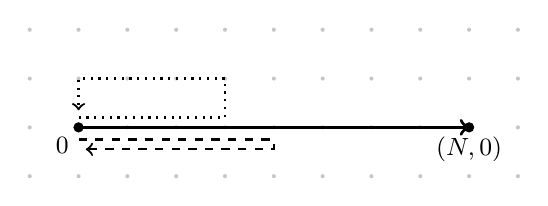
\begin{tikzpicture}[scale=0.62,font=\small]
 \foreach \x in {-1,...,9} \foreach \y in {-1,...,2} \fill[gray!45] (\x,\y) circle (1.2pt);
 \draw[very thick,->] (0,0) -- (8,0);
 \draw[thick,dashed,->] (0,-0.25) -- (4,-0.25) -- (4,-0.45) -- (0.15,-0.45);
 \draw[thick,dotted,->] (0,0.2) -- (3,0.2) -- (3,1) -- (0,1) -- (0,0.35);
 \fill (0,0) circle (3pt) node[below left] {$0$};
 \fill (8,0) circle (3pt) node[below] {$(N,0)$};
\end{tikzpicture}
\caption{Paths of $N=8$ steps. The only path to the corner $(N,0)$ never
switches (solid). A path to the origin either stays on one axis and only
reverses (dashed), or it turns and then uses all 4 directions (dotted).}
\label{fig:planarpaths}
\end{figure}

We write $u=sh/p_0$, $v=rh/p_0$ and $w=\beta h/p_0=2v+u$, so $1+w=1/p_0$. These
are the odds of a reversal, of a turn to a given side and of any switch, as in
the shared notation $u=q/p$. We use $S_N$, $u_N$, $p_N$, $z_N=N(1-p_N)$ and
$c_0$ from Section~\ref{sec:notation}. As $N$ is even, $S_N(u)$ is the sum of
$u^j$ over the words with $N/2$ letters of each of 2 kinds, where $j$ is the
number of switches. It has nonnegative coefficients and no constant term, so it
increases strictly on $[0,\infty)$.

\emph{The answer at first order.} Face selection predicts the answer, up to
powers of $\log N$. Let $h=\tau\log N/N$. The corner is the vertex $\{0\}$,
which has exit rate $\beta$, so $c_N$ is about $N^{-\beta\tau}$. A vertex, a
face with 3 directions, or a face with 2 adjacent ones misses the opposite of
one of its directions, so it cannot reach the origin. On the axis $\{0,2\}$,
which has exit rate $2r$, the origin is the single composition
$(N/2,0,N/2,0)$, of probability about $N^{-(2r\tau+1)}$. On the full face a
single composition has probability about $N^{-3}$, but about $N/2$
compositions $(a,b,a,b)$ end at the origin, and together they give about
$N^{-2}$. So the origin should beat the corner when $\beta\tau>\min(2r\tau+1,2)$,
that is, when $\tau>\tau^*=\min(2/\beta,1/s)$. At $\tau^*$ the axes win if
$s>2r$ and the full face wins if $s<2r$. This is only a heuristic, since it
applies Theorem~\ref{thm:first} to a linear function of the composition, which
we have not proved in general. Theorem~\ref{thm:planar-first} proves the
conclusion directly, and Theorem~\ref{thm:planar-rev} finds the crossing up to
$O(N^{-\gamma})$ when reversals dominate. The tool is a decomposition of a path
into 3 independent levels.

\begin{lemma}[3 levels]\label{lem:threelevel}
Write a sequence of directions as its number $m$ of switches, its skeleton $Z=(Z_0,\dots,Z_m)$,
which lists the directions of the runs so that $Z_t\ne Z_{t-1}$, and its run lengths
$\ell=(\ell_0,\dots,\ell_m)$, which form a composition of $N$ into $m+1$ positive parts. This is a
bijection, and $Y_N=\sum_{t=0}^m\ell_te_{Z_t}$. Under the walk, \textup{(a)} $m$ has the law
$\mathrm{Bin}(N-1,\beta h)$. Given $m$, \textup{(b)} $Z$ and $\ell$ are independent, \textup{(c)}
$Z$ is the random walk on $\Z_4$ with uniform $Z_0$ whose independent increments are $\pm1$ with
probability $r/\beta$ each and $2$ with probability $s/\beta$, and \textup{(d)} $\ell$ is uniform on
the $\binom{N-1}m$ compositions.
\end{lemma}

\begin{proof}
Put $q(\pm1)=r$ and $q(2)=s$. The sequence with data $(m,Z,\ell)$ has probability
\[
 \frac14p_0^{N-1-m}\prod_{t=1}^mh\,q(Z_t-Z_{t-1})
 =\binom{N-1}m(\beta h)^mp_0^{N-1-m}\cdot\frac14\prod_{t=1}^m\frac{q(Z_t-Z_{t-1})}\beta
 \cdot\binom{N-1}m^{-1}.
\]
For fixed $m$ the middle factor is the probability of $Z$ under the walk in (c), so it sums to $1$
over the skeletons, and the last factor sums to $1$ over the compositions. So the 3 factors are the
laws in (a), (c) and (d), and the product form gives (b).
\end{proof}

\begin{proposition}[exact decomposition and a unique crossing]\label{prop:decomp}
Let $N\ge2$ be even and $0<h<1/\beta$. Let $o^{(0)}_N$ and $o^{(4)}_N$ be the probabilities that
$Y_N=0$ and the walk never turns, and that $Y_N=0$ and the walk uses all 4 directions. Then
$o_N=o^{(0)}_N+o^{(4)}_N$,
\[
 o^{(0)}_N=2S_N(u)\,c_N,\qquad 0\le o^{(4)}_N\le\frac{w^2}{2p_0}\bigl(1-p_0^N\bigr).
\]
Equivalently, $o_N/c_N=2S_N(u)+E_N$ with $0\le E_N\le2w^2\bigl((1+w)^N-1\bigr)$. Also, $o_N/c_N$
is a polynomial in $v$ and $u$ with nonnegative coefficients and no constant term. If $s>0$, or if
$s=0$ and $N\ge4$, it increases strictly in $h$ from $0$ at $h=0$ to $\infty$ as $h\uparrow1/\beta$.
So there is exactly one $h^*_N\in(0,1/\beta)$ with $o_N=c_N$, and the corner is more likely than the
origin exactly when $h<h^*_N$.
\end{proposition}

In words: the origin mass splits exactly into the axis part, which is twice the
middle bin of Kagey's board measured against its endpoint, and a part from
paths with all 4 directions, which is small when $w$ is small. The ratio
$o_N/c_N$ grows with the switching rate, so the corner and the origin cross
exactly once, at every even $N\ge4$.

\begin{proof}
An origin path with no turn stays on the axis of its first step. An origin path that turns uses both
axes, and since $n_0=n_2$ and $n_1=n_3$ at the origin, it uses all 4 directions. So every origin
path is of exactly one of the 2 kinds. The origin paths on the axis $\{0,2\}$ are the paths with
$n_0=n_2=N/2$, and the path that always goes east has probability $c_N$. So
Proposition~\ref{prop:pair} with $a=s$ and $q=\beta$, for the pairs $\{0,2\}$ and $\{1,3\}$, gives
$o^{(0)}_N=2S_N(u)c_N$. The bound on $o^{(4)}_N$ follows from Lemma~\ref{lem:threelevel} and a count
of the run lengths that bring a skeleton back to the origin. We prove it in
Appendix~\ref{app:planar}. Dividing by $c_N$ gives the form with $E_N$.

A path with $a$ turns and $b$ reversals has probability $\frac14p_0^{N-1-a-b}(rh)^a(sh)^b=c_Nv^au^b$.
So $o_N/c_N$ is the sum of $v^au^b$ over the origin paths, and $a+b\ge1$ for each of them. Both $u$
and $v$ are nondecreasing in $h$, and each of them with a positive rate increases strictly to
$\infty$ as $h\uparrow1/\beta$. If $s>0$, the path that goes east $N/2$ times and then west gives
the term $u$. If $s=0$ and $N\ge4$, then $r>0$, and a path whose 4 runs go east, north, west and
south, with lengths $a,b,a,b\ge1$, gives the term $v^3$. This proves the claims on monotonicity and
the limits. For $s=0$ and $N=2$ the origin cannot be reached.
\end{proof}

The identity and the unique crossing for $s>0$ are checked in Lean (Section~\ref{sec:verify}). We
write $T^*_N=Nh^*_N$ and $u^*_N=sh^*_N/(1-\beta h^*_N)$. At the crossing $o_N=c_N$, so
$2S_N(u^*_N)=o^{(0)}_N/o_N$ there. We call it the zero-turn share of the origin mass.

We compare $S_N$ with Bessel functions by the uniform Bessel bound of~\cite{paperA}. Put
$\psi(z)=z(I_0(z)+I_1(z))$. In our notation that bound says that for every $N\ge2$ and $z>0$
\begin{equation}\label{eq:planar-bessel}
 \Bigl(1-\frac{z(z+2)}{2N}\Bigr)\psi(z)\le\frac N2\,S_N\Bigl(\frac zN\Bigr)\le\psi(z).
\end{equation}
Since $I_0'=I_1$ and $(zI_1)'=zI_0$, we have $\psi'=\psi+I_0$, so $(\log\psi)'\ge1$.

\begin{theorem}[first order]\label{thm:planar-first}
Fix $r>0$ and $s\ge0$, put $\tau^*=\min(2/\beta,1/s)$ with $1/0=\infty$, and let $N\to\infty$
through even integers.
\begin{enumerate}[(a)]
\item Fix $\tau>0$ and put $h=\tau\log N/N$. If $\tau<\tau^*$, then $o_N/c_N\le N^{-\gamma}$ for
some $\gamma>0$ and all large $N$. If $\tau>\tau^*$, then $o_N/c_N\ge N^{\gamma}$ for some
$\gamma>0$ and all large $N$.
\item $T^*_N/\log N\to\tau^*$.
\item If $s>2r$, then $2S_N(u^*_N)\to1$, so the origin mass at the crossing comes from the 2 axes,
half from each. If $s<2r$, then $2S_N(u^*_N)\le N^{-\gamma}$ for some $\gamma>0$ and all large $N$,
so it comes from the paths that use all 4 directions.
\end{enumerate}
\end{theorem}

In words, the heuristic above is right: the crossing sits at $T\approx\tau^*\log
N$, and at the crossing the origin is reached through the axes when reversals
dominate and through all 4 directions when turns dominate.

\emph{Idea of the proof.} The proof is in Appendix~\ref{app:planar}. The upper
bound in (a) follows from Proposition~\ref{prop:decomp} and
\eqref{eq:planar-bessel}. For the lower bound when $\beta\tau>2$ we count
balanced skeletons with Lemma~\ref{lem:threelevel}, and they give $o^{(4)}_N$ of
order at least $N^{-2}T^{-1/2}$. Part (b) follows from (a) and the monotonicity
in Proposition~\ref{prop:decomp}. For $r=0$ the same limit $1/s$ follows from
Theorem~\ref{thm:planar-rev}(c).

When reversals dominate, the crossing is the crossing of~\cite{paperA} for $N/2$ steps. We write
$z_{N/2}=\frac N2(1-p_{N/2})$ for it, and put
\[
 \mathcal A(\Lambda)=\Lambda-\tfrac12\log\Lambda+c_0
 +\frac{\frac14\log\Lambda-\frac12c_0+\frac18}{\Lambda},
\]
so that the third-order expansion of $z_N$ in~\cite{paperA} reads
$z_N=\mathcal A(L)+O((\log L)^2/L^2)$.

\begin{theorem}[reversals dominate]\label{thm:planar-rev}
\begin{enumerate}[(a)]
\item Let $s>0$. For all even $N\ge2$ and $0<h<1/\beta$,
\[
 \frac{o_N}{c_N}=2S_N(u)\bigl(1+\varepsilon_N(h)\bigr),\qquad
 0\le\varepsilon_N(h)\le\frac{w^2(1+w)^N}{S_N(u)}.
\]
\item Let $r\ge0$ and $s>2r$, let $N\to\infty$ through even integers, and let
$0<\gamma<\min(1,(s-2r)/s)$. Then
\[
 \varepsilon_N(h^*_N)=O\bigl((\log N)^{3/2-r/s}N^{-(s-2r)/s}\bigr),\qquad
 Nu^*_N=z_{N/2}+O(N^{-\gamma}).
\]
\item Under the hypotheses of (b), $sT^*_N=z_{N/2}+O(N^{-\gamma})$. Hence
\[
 sT^*_N=\mathcal A(L-\log2)+O\Bigl(\frac{(\log L)^2}{L^2}\Bigr),\qquad
 sT^*_N-z_N=-\log2+\frac{\log2}{2L}+O\Bigl(\frac{(\log L)^2}{L^2}\Bigr).
\]
\end{enumerate}
\end{theorem}

In words: when reversals dominate, the planar walk at its crossing behaves like
Kagey's board with half as many steps, and its crossing is smaller than
Kagey's by $\log2$ in the limit. Here is why. At the crossing $o_N\approx
o^{(0)}_N=2S_N(u)c_N$, so the 2 axes double the mass at the origin. By
\eqref{eq:planar-bessel}, applied with $N$ and with $N/2$ steps, the equations
$2S_N(z/N)=1$ and $S_{N/2}(z/(N/2))=1$ both say that $\psi(z)\approx N/4$. So
doubling $S_N$ has the same effect as halving $N$.

\begin{proof}
(a) Since $s>0$, $S_N(u)\ge2u>0$. Divide Proposition~\ref{prop:decomp} by $2S_N(u)$. Then
$\varepsilon_N(h)=E_N/(2S_N(u))$ and $E_N\le2w^2(1+w)^N$.

(b) Write $u^*=u^*_N$, $z^*=Nu^*$ and $E^*=E_N(h^*_N)$. At the crossing
Proposition~\ref{prop:decomp} gives $2S_N(u^*)+E^*=1$. So $S_N(u^*)\le\frac12<S_N(u_N)$, and
$u^*<u_N$. Put $w_N=\beta u_N/s$. Since $w\mapsto2w^2(1+w)^N$ is increasing,
$E^*\le\eta_N:=2w_N^2(1+w_N)^N$. By the second-order expansion of $z_N$ in~\cite{paperA},
$Nu_N=z_N/p_N=L-\frac12\log L+O(1)$. So $(1+w_N)^N\le e^{Nw_N}=O(N^{\beta/s}L^{-\beta/(2s)})$ and
$w_N^2=O(L^2/N^2)$. As $\beta/s-2=-(s-2r)/s$ and $2-\beta/(2s)=\frac32-\frac rs$, this gives
$\eta_N=O(L^{3/2-r/s}N^{-(s-2r)/s})$, which tends to $0$. Then
$\varepsilon_N(h^*_N)=E^*/(1-E^*)\le\eta_N/(1-\eta_N)$.

Next let $z'=\frac N2u_{N/2}$, so that $S_{N/2}(2z'/N)=1$. By \eqref{eq:planar-bessel} with
$N/2$ steps, $\frac N4\le\psi(z')\le\frac N4(1-\delta'_N)^{-1}$ with $\delta'_N=z'(z'+2)/N$. By
\eqref{eq:planar-bessel} with $N$ steps and $\frac12(1-\eta_N)\le S_N(u^*)\le\frac12$, we get
$\frac N4(1-\eta_N)\le\psi(z^*)\le\frac N4(1-\delta_N)^{-1}$ with $\delta_N=z^*(z^*+2)/(2N)$. Both $z'$
and $z^*<Nu_N$ are $O(L)$, so $\delta_N,\delta'_N=O(L^2/N)$. As $(\log\psi)'\ge1$,
$\lvert z^*-z'\rvert\le\lvert\log\psi(z^*)-\log\psi(z')\rvert=O(\eta_N+L^2/N)$. Finally
$z_{N/2}=z'/(1+u_{N/2})=z'+O(L^2/N)$. So $z^*-z_{N/2}=O(\eta_N+L^2/N)$, which is $O(N^{-\gamma})$.

(c) Since $h^*_N=u^*/(s+\beta u^*)$, we have $sT^*_N=z^*/(1+\beta u^*/s)=z^*+O(L^2/N)$, as
$u^*<u_N=O(L/N)$. With (b) this gives $sT^*_N=z_{N/2}+O(N^{-\gamma})$. The third-order expansion of
$z_N$ in~\cite{paperA}, for $N/2$ steps and for $N$ steps, gives
$z_{N/2}=\mathcal A(L-\log2)+O((\log L)^2/L^2)$ and $z_N=\mathcal A(L)+O((\log L)^2/L^2)$. The last
term of $\mathcal A$ has derivative $O(\log L/L^2)$ near $L$, so
\[
 \mathcal A(L-\log2)-\mathcal A(L)=-\log2-\tfrac12\log\Bigl(1-\frac{\log2}L\Bigr)
 +O\Bigl(\frac{\log L}{L^2}\Bigr)=-\log2+\frac{\log2}{2L}+O\Bigl(\frac{\log L}{L^2}\Bigr).
\qedhere
\]
\end{proof}

For $(r,s)=(0.1,1)$ the difference $sT^*_N-z_N$ is $-0.6317$ at $N=640$ and $-0.6493$ at
$N=10240$, while the first 2 terms in (c) give $-0.6395$ and $-0.6556$ (Figure~\ref{fig:planar}(a)).
When turns dominate, the origin mass is carried by the paths with all 4 directions, and we need
their local limit.

\begin{remark}[when turns matter, proof omitted]\label{rem:planar-turns}
Let $r>0$ and $s\ge0$, let $N\to\infty$ through even integers, and let $T=Nh\to\infty$ with
$T\le N^{1/8}$. Then $N^2o^{(4)}_N=\frac{2(r+s)}\pi T(1+o(1))$. This is twice the density at $0$ of
a centered Gaussian vector with covariance $\frac{N^2}{2(r+s)T}I_2$, and the factor $2$ appears
because $Y_N$ lies on a sublattice of index $2$. If $s<2r$, it gives
\[
 \beta T^*_N+\log T^*_N=2L+\log\frac\pi{8(r+s)}+o(1),\qquad\text{or}\qquad
 \beta T^*_N=2z_N+\log\frac\beta{2(r+s)}+o(1).
\]
For $r=s=1$ the bold curve of Figure~\ref{fig:program} solves the first equation without its
$o(1)$ term. The coefficient of $\log T^*_N$ is $1$ and not $\frac12$, because the origin is a point of a
2-dimensional local limit. Still $T^*_N=\tau^*[L-\frac12\log L+O(1)]$ for every $s\ge0$. At the
switch $s=2r$ the zero-turn share tends to $2\sqrt2/(\sqrt2+\sqrt5)=0.7749$, and the term
$\log((\sqrt5-\sqrt2)/(\sqrt5+\sqrt2))$ is added to the right side of the first equation. The
approach is slow. At $N=10240$ the zero-turn share is $0.7650$ for $(r,s)=(0.5,1)$ and still
$0.1051$ for $(1,1)$ (Figure~\ref{fig:planar}(b)). With turns only ($s=0$), we rotate the lattice
by $45^\circ$. If $Y_N=(Y^{(1)},Y^{(2)})$, then $Y^{(1)}+Y^{(2)}$ and $Y^{(1)}-Y^{(2)}$ move by
$\pm1$ at each step, and their sign words are 2 copies of the walk of~\cite{paperA} that never
switch at the same step. So $Y_N=0$ exactly when both words are balanced, which is the lattice form
of the factorization in~\cite[Eq.~(36)]{angelani2022}. A union bound over the pairs of balanced
words that switch at a common step then gives $rT^*_N=z_N+O((\log N)^4/N)$. The other proofs use
Lemma~\ref{lem:threelevel}, a local limit for the run lengths given the skeleton and a martingale
central limit theorem~\cite{hallheyde1980} for the skeleton. We omit the details.
\end{remark}

\begin{figure}[t]
\centering
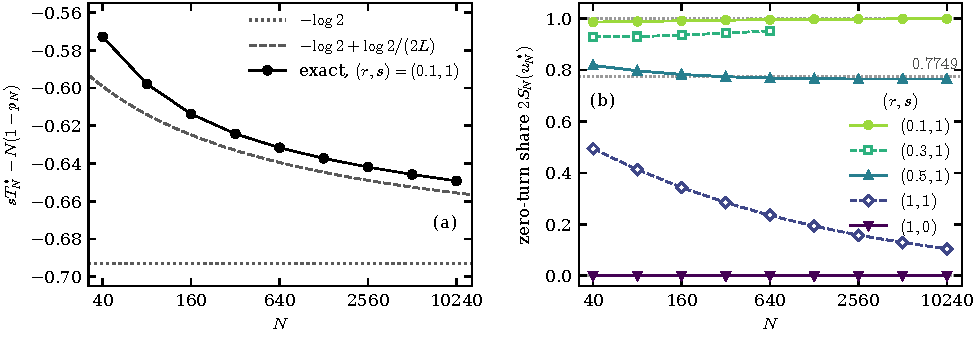
\includegraphics[width=\textwidth]{fig_planar}
\caption{(a) The exact crossing of the planar walk with $(r,s)=(0.1,1)$, written as
$sT^*_N-z_N$ with $z_N=N(1-p_N)$, for $N=40,80,\dots,10240$. The dashed curve is
$-\log2+\log2/(2L)$ from Theorem~\ref{thm:planar-rev}(c), and the dotted line is its limit $-\log2$.
(b) The zero-turn share $2S_N(u^*_N)$ of the origin mass at the crossing. It tends to $1$ for
$s>2r$ and to $0$ for $s<2r$ (Theorem~\ref{thm:planar-first}), and by
Remark~\ref{rem:planar-turns} (proof omitted) to $2\sqrt2/(\sqrt2+\sqrt5)=0.7749$ at the switch
$s=2r$. For $(r,s)=(1,0)$ there are no reversals and
the share is $0$ for every $N$. The pair $(0.3,1)$ was computed up to $N=640$.}
\label{fig:planar}
\end{figure}

\section{Application: sticky priors for hidden Markov models}\label{sec:sticky}

This section is an application for readers from statistics. Nothing earlier
depends on it, and a reader who is interested only in the general theory and
the planar walk can skip to Section~\ref{sec:verify}.

In a hidden Markov model the hidden states $X_1,\dots,X_N$ form a Markov chain
on $d$ states. Before any data are seen, the model already says how the $N$
time steps are likely to be shared among the states. This is the law $P_N$ of
the count vector $n=(n_1,\dots,n_d)$, where $n_i$ is the number of time steps in
state $i$ (the composition of Section~\ref{sec:model}). A sticky prior makes
the chain leave its current state rarely, which is the regime of this paper.
We ask which states the most likely count vector uses.

Here is what we use from the earlier sections. Suppose the chain leaves its
state with probability $h=\tau\log N/N$ at each step and then picks the next
state from a kernel $\Pi$. For a set $F$ of states (a face) let $\rho_F$ be
the Perron root of $\Pi$ restricted to $F$. The chain stays in $F$ for all $N$
steps with probability about $N^{-\tau(1-\rho_F)}$, and about $N^{|F|-1}$ count
vectors use exactly the states of $F$. Theorem~\ref{thm:first} says that for
large $N$ the most likely count vector uses a set $F$ that minimizes
$\Phi_\tau(F)=\tau(1-\rho_F)+|F|-1$, and that its fractions $n/N$ are then
close to the law $\alpha^*_F$, the entrywise product of the left and right
Perron vectors of $\Pi$ on $F$. Besides this we use the description of a tie
between several minimizers (Theorem~\ref{thm:window}) and the exact identity
for a symmetric pair of states (Proposition~\ref{prop:pair}), once each.

The answer is as follows. As the stickiness decreases, that is, as $\tau$
grows, the most likely count vector moves from one state to larger sets of
states. Among symmetric kernels only the uniform one jumps from one state
straight to all of them.

Fox et al.~\cite{fox2011} add a self-transition bias $\kappa\ge0$ to the HDP
hidden Markov model (HDP stands for hierarchical Dirichlet process), so that
the hidden chain stays in each state longer. In their weak-limit approximation
with base weights $\bar\beta$ and concentration $\omega$, row $j$ of the
transition matrix is Dirichlet with parameters
$\omega\bar\beta_1,\dots,\omega\bar\beta_j+\kappa,\dots,\omega\bar\beta_d$. By
neutrality, row $j$ off the diagonal, divided by $1-\pi_{jj}$, is Dirichlet
with parameters $(\omega\bar\beta_l)_{l\ne j}$ and independent of $\pi_{jj}$. So
$\kappa$ only sets how sticky the chain is, and the kernel of the switches does
not depend on it. In this section we fix every exit probability $1-\pi_{jj}$ at
the same value $h=\tau L/N$, the scale of Kagey's crossing, and study the
kernel. The prior itself mixes over all values of the exit probabilities, and
we do not treat this mixture.

So let $\Pi=(\pi_{ij})$ be a stochastic matrix on $[d]$ with zero diagonal,
$\tau>0$ and $h=\tau L/N<1$. The hidden chain has transition matrix
$(1-h)I+h\Pi=I+hQ$ with $Q=\Pi-I$, so
$q_i=1$ and $T=\tau L$ (Example~\ref{ex:models}(iii)). We assume that
$\pi_{ij}>0$ for all $i\ne j$, which we call (A+), and that the start $\mu$ has
full support. Under the prior (A+) holds almost surely. Let
$\rho_F=\varrho(\Pi_F)$ for the principal submatrix $\Pi_F$ on $F$. Then the
exit rate of $F$ is $\lambda_F=1-\rho_F$, and
$Q_F$ and $\Pi_F$ have the same Perron vectors. A vertex (a single state) has
$\rho_F=0$, and
$\rho_{[d]}=1$. If $2\le|F|\le d-1$, then $\Pi_F$ is irreducible by (A+), and
$0<\rho_F<1$ since $\rho_F$ is at least the least row sum of $\Pi_F$ and the
Perron root of the irreducible $\Pi$ exceeds that of each proper principal
submatrix~\cite{bermanplemmons1994}. So
$\Phi_\tau(F)=\tau(1-\rho_F)+|F|-1$, and we put
\[
 \tau_-=\min_{|F|\ge2}\frac{|F|-1}{\rho_F},\qquad
 \tau_+=\max_{F\ne[d]}\frac{d-|F|}{1-\rho_F}.
\]
We call a global mode of $P_N$, that is, a most likely value of the count
vector before any data are seen, a \emph{prior mode}.

\begin{corollary}[support and location of the prior mode]\label{cor:map}
Assume \textup{(A+)}, let $\mu$ have full support, and fix $\tau>0$. Let
$\mathcal F_\tau$ be the set of faces that minimize $\Phi_\tau$. There is
$N_0(\tau)$ such that for $N\ge N_0(\tau)$ every prior mode $n^*$
satisfies $\supp n^*\in\mathcal F_\tau$ and $n^*/N=\alpha^*_F+O(1/L)$ with
$F=\supp n^*$. If $\mathcal F_\tau=\{F^*\}$, then
$n^*/N\to\alpha^*_{F^*}=l\circ r$, where $l$ and $r$ are the left and right
Perron vectors of $\Pi_{F^*}$ with $l\cdot r=1$. No reversibility is needed.
\end{corollary}

In words, for large $N$ a prior mode uses exactly the states of a set that
minimizes $\Phi_\tau$, and it shares the $N$ time steps among them in the
proportions $\alpha^*_F$.

\begin{proof}
By (A+) every face is irreducible and, as $\mu$ has full support,
admissible. So Theorem~\ref{thm:first}(iii) and~(iv) give the claims, with
$\alpha^*_F=l\circ r$.
\end{proof}

The threshold $N_0(\tau)$ is not uniform in $\tau$. At $\tau=\tau_-$ the
vertices tie with the faces that attain $\tau_-$, and
Theorem~\ref{thm:window}(iii) with $\tau^*=\tau_-$ and a fixed large $t=t_0$
shows that for large $N$ the prior mode is not a single state at
$\tau=\tau_-(1-\frac{\log L-2t_0}{2L})<\tau_-$. So $N_0(\tau)\to\infty$ as
$\tau\uparrow\tau_-$.

The next proposition says for which $\tau$ the prior mode uses one state, all
states, or a set in between.

\begin{proposition}[thresholds]\label{prop:thresholds}
Assume \textup{(A+)} and $d\ge3$.
\begin{enumerate}[(a)]
\item The minimizers of $\Phi_\tau$ are exactly the vertices if and only if
$\tau<\tau_-$, and no vertex minimizes $\Phi_\tau$ if $\tau>\tau_-$. The face
$[d]$ is the unique minimizer if and only if $\tau>\tau_+$, and $[d]$ does not
minimize $\Phi_\tau$ if $\tau<\tau_+$.
\item $1<\tau_-\le d-1\le\tau_+$.
\item $\tau_-=d-1$ if and only if $\tau_+=d-1$, and both hold if and only if
\begin{equation}\label{eq:directjump}
 \rho_F\le\frac{|F|-1}{d-1}\qquad\text{for every face } F.
\end{equation}
If \eqref{eq:directjump} fails, then $\tau_-<d-1<\tau_+$, and for
$\tau\in(\tau_-,\tau_+)$ every minimizer $F$ of $\Phi_\tau$ has
$2\le|F|\le d-1$.
\end{enumerate}
Consequently, let $\mu$ have full support, fix $\tau$ and let $N\ge N_0(\tau)$
as in Corollary~\ref{cor:map}. If $\tau<\tau_-$, the prior
modes are the $Ne_i$ with $\mu_i=\max_l\mu_l$. If $\tau>\tau_+$, every
prior mode has full support. If $\tau_-<\tau<\tau_+$, every prior
mode has a support $F$ with $2\le|F|\le d-1$, and $F=F^*$ if $F^*$ is
the unique minimizer of $\Phi_\tau$.
\end{proposition}

\begin{proof}
We compare every face with a vertex and with $[d]$. The function
$\Phi_\tau(F)=\tau(1-\rho_F)+|F|-1$ is affine in $\tau$, so each comparison
changes sign at one value of $\tau$, and $\tau_-$ and $\tau_+$ are the extreme
ones.

(a) A vertex has $\Phi_\tau=\tau$. For $|F|\ge2$ we have $\rho_F>0$ and
\[
 \Phi_\tau(F)-\tau=|F|-1-\tau\rho_F=\rho_F\Bigl(\frac{|F|-1}{\rho_F}-\tau\Bigr).
\]
So $F$ is worse than a vertex exactly when $\tau<(|F|-1)/\rho_F$. This holds
for every $F$ with $|F|\ge2$ exactly when $\tau<\tau_-$, and if $\tau>\tau_-$
some $F$ is better than every vertex. In the same way $\Phi_\tau([d])=d-1$,
and for $F\ne[d]$ we have $1-\rho_F>0$ and
\[
 \Phi_\tau(F)-(d-1)=\tau(1-\rho_F)-(d-|F|)
 =(1-\rho_F)\Bigl(\tau-\frac{d-|F|}{1-\rho_F}\Bigr).
\]
So $F$ is worse than $[d]$ exactly when $\tau>(d-|F|)/(1-\rho_F)$, which gives
the two claims on $[d]$.

(b) In the minimum that defines $\tau_-$, a face with $2\le|F|\le d-1$ has
$\rho_F<1$ and so $(|F|-1)/\rho_F>1$, and $[d]$ gives the value $d-1\ge2$. So
$\tau_->1$ and $\tau_-\le d-1$. In the maximum that defines $\tau_+$, a vertex
gives the value $d-1$, so $\tau_+\ge d-1$.

(c) By (b), $\tau_-=d-1$ exactly when $(|F|-1)/\rho_F\ge d-1$ for all
$|F|\ge2$, and $\tau_+=d-1$ exactly when $(d-|F|)/(1-\rho_F)\le d-1$ for all
$F\ne[d]$. After clearing the denominators both conditions say
$(d-1)\rho_F\le|F|-1$. This inequality always holds for the vertices and for
$[d]$, so each condition is \eqref{eq:directjump}. If
\eqref{eq:directjump} fails, then neither holds, so $\tau_-<d-1<\tau_+$ by
(b), and (a) excludes the vertices and $[d]$ on $(\tau_-,\tau_+)$.

For the consequence, Corollary~\ref{cor:map} says that the support of a prior
mode minimizes $\Phi_\tau$, and (a) and (c) say which faces can do so. If
$\tau<\tau_-$ the prior modes are vertex compositions, and
$P_N(Ne_i)=\mu_i(1-h)^{N-1}$ is largest for the largest $\mu_i$. Parts (a) to
(c) are checked in Lean.
\end{proof}

We say that $\Pi$ has a \emph{direct jump} when \eqref{eq:directjump} holds.
Then at first order the prior mode goes from one state straight to all $d$ states at
$\tau=d-1$. For the uniform kernel $\pi_{ij}=1/(d-1)$ the matrix $\Pi_F$ has
constant row sums, so $\rho_F=(|F|-1)/(d-1)$. Hence
\eqref{eq:directjump} says that no set of states is more closed than under the
uniform kernel. That kernel has $Q=(J-dI)/(d-1)$, and all its faces tie at
$\tau=d-1$. This is the degeneracy of~\cite{paperB} (Corollary~\ref{cor:paperB}).
The next corollary shows that a direct jump is special.

\begin{corollary}[only the uniform kernel]\label{cor:uniform-kernel}
Let $d\ge3$ and assume \textup{(A+)}. \textup{(a)} If $\Pi$ is symmetric,
then $\Pi$ has a direct jump if and only if $\pi_{ij}=1/(d-1)$ for all
$i\ne j$. \textup{(b)} If $d=3$, then $\Pi$ has a direct jump if and only if
$\pi_{ij}\pi_{ji}\le\frac14$ for all three pairs. In particular every cyclic
kernel $\pi_{i,i+1}=a$, $\pi_{i,i-1}=1-a$ (indices mod $3$) has a direct
jump.
\end{corollary}

\begin{proof}
We test \eqref{eq:directjump} on the pairs. The matrix $\Pi_{\{i,j\}}$ has
zero diagonal and off-diagonal entries $\pi_{ij}$ and $\pi_{ji}$, so
$\rho_{\{i,j\}}=\sqrt{\pi_{ij}\pi_{ji}}$.

(a) Here $\rho_{\{i,j\}}=\pi_{ij}$, so for a pair \eqref{eq:directjump} reads
$\pi_{ij}\le1/(d-1)$. The $d$ rows sum to $1$ and have $d(d-1)$ off-diagonal
entries, so the average of the $\pi_{ij}$ is $1/(d-1)$. If none of them
exceeds the average, they are all equal to it. So a direct jump forces the
uniform kernel. Conversely the uniform kernel has $\rho_F=(|F|-1)/(d-1)$ for
every face, as we saw above, so it satisfies \eqref{eq:directjump} with
equality.

(b) For $d=3$ the faces are the vertices, the three pairs and $[3]$. For the
vertices and $[3]$, \eqref{eq:directjump} reads $0\le0$ and $1\le1$. For a
pair it reads $\sqrt{\pi_{ij}\pi_{ji}}\le\frac12$. The cyclic kernel has
$\pi_{ij}\pi_{ji}=a(1-a)\le\frac14$ for every pair. Both parts are checked in
Lean.
\end{proof}

So for a symmetric kernel that is not uniform there is a range of $\tau$ in
which the prior mode uses more than one state but not all of them
(Proposition~\ref{prop:thresholds}(c)). Without symmetry a direct jump is
possible, and for three states we can say how likely it is under the prior.

\begin{proposition}[the direct jump under the prior]\label{prop:directjump}
Let $d=3$ and let the base weights be uniform. In the weak-limit sticky
HDP-HMM the rows of $\Pi$ are then independent, and the first off-diagonal
entry of each row has the law $\mathrm{Beta}(\omega/3,\omega/3)$. Write
$\Prob_\omega$ for this law of $\Pi$ and $D$ for the event that $\Pi$ has a
direct jump. Then \textup{(a)} $\Prob_\omega(D)\to\frac14$ as $\omega\to0$,
and \textup{(b)} $\Prob_\omega(D)=\frac{3\sqrt3}{8\pi\omega}(1+o(1))$ as
$\omega\to\infty$.
\end{proposition}

\begin{proof}
Let $B_1,B_2,B_3$ be independent with law $\mathrm{Beta}(\omega/3,\omega/3)$,
and put $\pi_{12}=B_1$, $\pi_{21}=B_2$ and $\pi_{31}=B_3$, so that the other
off-diagonal entries are $1-B_j$. By Corollary~\ref{cor:uniform-kernel}(b),
$D$ is the event that $B_1B_2$, $(1-B_1)B_3$ and $(1-B_2)(1-B_3)$ are all at
most $\frac14$.

(a) As $\omega\to0$ each $B_j$ tends in law to a fair coin on $\{0,1\}$. So
the law of $(B_1,B_2,B_3)$ tends to the uniform law on the eight points of
$\{0,1\}^3$. At these points the three products take only the values $0$ and
$1$, so none of the points lies on the boundary of $D$ (where some product
equals $\frac14$). Hence $\Prob_\omega(D)$ tends to the limit probability of
$D$, which is the fraction of the eight points at which all three products are
$0$. Only $(1,0,1)$ and $(0,1,0)$ have this property (checked in Lean), so the
limit is $\frac28=\frac14$. Part (b) is proved in Appendix~\ref{app:hdp}.
\end{proof}

In words, a direct jump has probability close to $\frac14$ when the
concentration is small and of order $1/\omega$ when it is large. For (b), for
large $\omega$ the set $D$ is a thin tube around the cyclic kernels, with
cross-section of area about $\frac98t^4$ at the logit coordinate $t$ along the
cyclic kernels (Appendix~\ref{app:hdp}), which gives the order $1/\omega$. So
the uniform tie is not typical. At $\omega=1$, Monte Carlo with $10^6$ draws
gives $\Prob_\omega(D)=0.115$. So about $0.88$ of random kernels have a range
of $\tau$ in which, at first order, the prior mode sits on a pair
(Proposition~\ref{prop:thresholds}(c)).

The comparison of a single state with a symmetric pair is exact at every $N$.

\begin{corollary}[an exact link to Kagey's crossing]\label{cor:sticky-pair}
Let $i\ne j$ satisfy $\pi_{ij}=\pi_{ji}=\pi_0>0$ and $\mu_i=\mu_j>0$. We do not
assume \textup{(A+)}. Then for every $N\ge2$ the balanced compositions are the
most likely ones with support $\{i,j\}$, and they are more likely than $Ne_i$
if and only if $\tau>\tau^{\rm pair}(N):=Nu_N/((\pi_0+u_N)L)$. If also
$\mu_i=\mu_j=\max_l\mu_l$, then for every $\tau$ with
$\tau^{\rm pair}(N)<\tau<N/L$ no prior mode is a single state. Moreover,
\[
 \tau^{\rm pair}(N)=\frac1{\pi_0}\Bigl[1-\frac{\frac12\log L-c_0}{L}
 +O\Bigl(\frac{\log L}{L^2}\Bigr)\Bigr],
\]
which tends to the first-order value $1/\rho_{\{i,j\}}=1/\pi_0$.
\end{corollary}

In words, a single state against a symmetric pair is Kagey's board, so the
value of $\tau$ at which the pair overtakes the state is known at every $N$ and
not only in the limit.

\begin{proof}
We apply Proposition~\ref{prop:pair}. Every exit rate is $1$, so its
hypotheses hold with $a=\pi_0$ and $q=1$, and its odds are $u=\pi_0h/(1-h)$. It
says that the balanced compositions are the most likely ones on $\{i,j\}$ and
that they beat $Ne_i$ exactly when $u>u_N$. Solving for $h$, this is
$h>u_N/(\pi_0+u_N)$, and with $h=\tau L/N$ it is $\tau>\tau^{\rm pair}(N)$.

For the prior modes, $P_N(Ne_l)=\mu_l(1-h)^{N-1}\le P_N(Ne_i)$ for every $l$.
So when the pair beats $Ne_i$ it beats every single state. The condition
$\tau<N/L$ is $h<1$, and the range of $\tau$ is not empty as
$u_N/(\pi_0+u_N)<1$.

Finally $Nu_N=z_N/p_N$ and $u_N=O(L/N)$, so
$\tau^{\rm pair}(N)=\frac{z_N}{\pi_0L}(1+O(L/N))$, and the second-order
expansion of $z_N$ in~\cite[Corollary~3.7(b)]{paperA} gives the claim.
\end{proof}

So far we looked at the single most likely count vector. The last result
gives the total probability that the chain uses only the states of a set $F$.

\begin{proposition}[face masses]\label{prop:mass}
Assume \textup{(A+)} and $0<h<1$. For every face $F$ with $|F|\ge2$ and
$\Lambda_F=1-h\lambda_F$,
\[
 \frac{\min r_F}{\max r_F}\mu(F)\Lambda_F^{N-1}
 \le\Prob(\supp n\subseteq F)\le
 \frac{\max r_F}{\min r_F}\mu(F)\Lambda_F^{N-1},
\]
and for fixed $\tau$, $\Lambda_F^{N-1}=N^{-\tau\lambda_F}e^{O(L^2/N)}$. Also
$\Prob(\text{one state})=(1-h)^{N-1}\sim N^{-\tau}$ and
$\Prob(\supp n=[d])\to1$ for fixed $\tau$.
\end{proposition}

In words, the chain stays inside $F$ with probability
$\mu(F)N^{-\tau\lambda_F}$ up to a bounded factor, and the probability that it
uses every state tends to $1$.

\begin{proof}
We write the probability with the transition matrix restricted to $F$ and
compare the vector $\ones$ with the Perron vector. Let
$U_F=(1-h)I+h\Pi_F\ge0$. The chain stays in $F$ for all $N$ steps with
probability $\Prob(\supp n\subseteq F)=\mu_F^{\top}U_F^{N-1}\ones$, and
$U_Fr_F=\Lambda_Fr_F$. As $r_F/\max r_F\le\ones\le r_F/\min r_F$ entrywise and
$U_F^{N-1}$ has nonnegative entries, we may replace $\ones$ by these two
multiples of $r_F$. This gives the bounds. For fixed $\tau$,
$(N-1)\log(1-h\lambda_F)=-\tau\lambda_FL+O(L^2/N)$. A vertex composition is a
single path that never switches, which gives $\Prob(\text{one state})$. Every
$F\ne[d]$ has $\lambda_F>0$, so each of the finitely many proper faces has
probability tending to $0$, and $\Prob(\supp n=[d])\to1$. The finite bounds are
checked in Lean.
\end{proof}

\begin{remark}[prior mode versus mass]\label{rem:mapmass}
Let $d\ge3$. For fixed $\tau<\tau_+$ and large $N$ every prior mode has a
proper support, while $\Prob(\supp n=[d])\to1$. For $\tau<\tau_-$ the prior mode uses
one state, an event of probability about $N^{-\tau}$. A face of size $k$ holds
about $N^{k-1}$ compositions, so it can carry most of the mass while each of
them is less likely than a vertex. Table~\ref{tab:sticky} shows this. At
$\tau=0.8$ the prior mode is a single state, yet $\Prob(\text{one state})=0.0122$. At
$\tau=8$ first
order puts the prior mode on $\{1,2\}$, but at $N=240$ it has full support. So the
prior mode can be a poor summary of a sticky prior, and face selection tells us
on which states it sits.
\end{remark}

\begin{table}[t]
\centering\small
\begin{tabular}{@{}rlccc@{}}
\toprule
$\tau$ & prior mode & one state & $\{1,2\}$ & $[3]$\\
\midrule
0.5 & one state & 0.0643 & 0.465 & 0.379\\
0.8 & one state & 0.0122 & 0.423 & 0.531\\
3 & $(120,120,0)$ & $4.3\times10^{-8}$ & 0.129 & 0.871\\
8 & $(111,111,18)$ & $1.2\times10^{-21}$ & 0.0081 & 0.992\\
\bottomrule
\end{tabular}
\caption{The kernel $\Pi$ with rows $(0,0.9,0.1)$, $(0.9,0,0.1)$,
$(0.5,0.5,0)$, the uniform start and $N=240$, where $\tau_-=10/9$ and
$\tau_+=10$. The prior mode (from exact dynamic programming, with a tie of
three compositions at $\tau=0.5$ and $0.8$) and the prior probabilities of the supports.}
\label{tab:sticky}
\end{table}

\section{Application: the information in the endpoint}\label{sec:fisher}

This second application returns to Kagey's board and asks a statistical
question. If we only see the bin where the ball lands, how much do we learn
about the switching probability? The answer is that the bin keeps about a
fraction $1/(2T)$ of the Fisher information of the whole path, so about
$1/(2\log N)$ at Kagey's crossing. We use the shared notation of
Section~\ref{sec:series}: the first step is left or right with probability
$\frac12$ each, and each later step repeats the one before it with probability
$p=1-q$, where $0<q<1$. This is Example~\ref{ex:models}(i) with $h=q$, so
$T=Nq$. Put $\rho=1-2q$, $u=q/p$ and $y=Nu=T/p$. Let $J$ be the number of
switches, $K$ the number of right steps, $X=2K-N$ the endpoint and $W=X/N$. A path with $J$ switches has probability
$\frac12p^{N-1-J}q^J$. So $J\sim\operatorname{Bin}(N-1,q)$, and the path
carries the Fisher information $(N-1)/(pq)$ about $q$. The endpoint carries
$I_K(q)=\sum_{k=0}^N(\partial_q\Prob(K=k))^2/\Prob(K=k)$, and we call
$e_N(q)=I_K(q)\,pq/(N-1)$ the \emph{efficiency} of the endpoint. It is the
fraction of the information left when we see only the endpoint.

The endpoint sees the switches only through how far the walk spreads. A
normal $X$ with mean $0$ and variance $Np/q$, close to $\Var X$ for large
$T$, would carry the information $\frac12(\partial_q\log(Np/q))^2=1/(2p^2q^2)$,
which is the fraction $1/(2(N-1)pq)\approx1/(2T)$. Theorem~\ref{thm:fisher}
confirms this.

\begin{proposition}[a correlation ratio]\label{prop:eta}
For $N\ge2$ and $0<q<1$,
\[
 e_N(q)=\frac{\Var(\E[J\mid K])}{\Var J}.
\]
For $0<k<N$ we have $\E[J\mid K=k]=\frac{d}{dt}\log S_{k,N-k}(e^t)$ at
$t=\log(q/p)$, where $S_{a,b}$ is the polynomial of
Section~\ref{sec:papersAB}. For $k\in\{0,N\}$ we have $J=0$.
\end{proposition}

\begin{proof}
The score of a path is $(J-(N-1)q)/(pq)$. Since $\Prob(K=k)$ is a sum of path
probabilities, $\partial_q\log\Prob(K=k)=\E[(J-(N-1)q)/(pq)\mid K=k]$. As
$\E J=(N-1)q$, this gives $I_K(q)=\Var(\E[J\mid K])/(pq)^2$, and we divide by
$(N-1)/(pq)=\Var J/(pq)^2$. By the run count of~\cite{paperA}, for $0<k<N$
the probability $\Prob(K=k,J=j)$ is $\frac12p^{N-1}u^j$ times the number of
words with $k$ right steps, $N-k$ left steps and $j$ switches. Summing over
$j$ gives $\Prob(K=k)=\frac12p^{N-1}S_{k,N-k}(u)$, so
$\E[J\mid K=k]=uS'_{k,N-k}(u)/S_{k,N-k}(u)$. Only the 2 constant paths have
$K\in\{0,N\}$.
\end{proof}

This identity, checked in Lean, says that $e_N$ is the correlation ratio of
$J$ on $K$. Since $\E[J\mid K]$ is the orthogonal projection of $J$ onto
the functions of $K$ in $L^2$, the Cauchy--Schwarz inequality gives
\begin{equation}\label{eq:fisher-proj}
 e_N(q)\ge\frac{\Cov(J,g(K))^2}{\Var J\,\Var g(K)}
 \qquad\text{whenever }\Var g(K)>0.
\end{equation}

\begin{remark}[few switches, proof omitted]\label{rem:fisher-small}
For fixed $N$ we have $e_N(q)=1-\frac{N-2}2q+O_N(q^2)$ as $q\to0$. If $q\to0$
and $T=Nq$ stays bounded, then $e_N(q)\to1$ if and only if $T\to0$. The
reason is that 1 switch and 2 switches both leave the endpoint uniform on the
interior bins. The proof applies \eqref{eq:fisher-proj} to the indicator of
$K\in\{0,N\}$ and compares the 2 words with 1 switch with the $N-2$ words
with 2 switches in each interior bin. We omit the details.
\end{remark}

\begin{theorem}[many switches]\label{thm:fisher}
Let $R^2_N(q)=\Cov(J,X^2)^2/(\Var J\,\Var X^2)$ be the squared correlation
of $J$ and $X^2$. For $N\ge2$ and $0<q<1$,
\[
 R^2_N(q)=\frac1{2(N-1)pq}\cdot
 \frac{\bigl[1+\rho^N-p(1-\rho^N)/T\bigr]^2}{V},
\]
where
\[
 V=1-\frac{1+8\rho+\rho^2+8\rho^{N+1}}{4pT}
 +\frac{\rho(1-\rho^N)\bigl[2(1+2\rho)(2+\rho)-\rho(1-\rho^N)\bigr]}{8p^2T^2}.
\]
There are absolute constants $C$ and $N_0$ such that for $N\ge N_0$,
$0<q\le\frac12$ and $1\le T\le N^{1/4}$,
\[
 0\le e_N(q)-R^2_N(q)\le C\Bigl(\frac1{T^3}+\frac{T^3}N\Bigr).
\]
Consequently, in the same range and with an absolute implied constant,
\[
 e_N(q)=\frac1{2T}+\frac1{4T^2}+O\Bigl(\frac1{T^3}+\frac{T^3}N\Bigr).
\]
\end{theorem}

In words, when $T$ is large but at most $N^{1/4}$, the endpoint keeps about the
fraction $1/(2T)$ of the information, and almost all of what it keeps is carried
by the single statistic $X^2$. The lower bound $e_N\ge R^2_N$ is
\eqref{eq:fisher-proj} with $g(K)=X^2$,
for all $N\ge2$ and $0<q<1$. For the upper bound, Proposition~\ref{prop:eta}
and the uniform Bessel estimate for every bin in~\cite{paperA} make
$\E[J\mid K]$ close to $y\sqrt{1-W^2}+\frac12$. As $W$ is of order
$T^{-1/2}$, this is close to $y(1-W^2/2)+\frac12$, which lies in the span of
$1$ and $X^2$. Appendix~\ref{app:fisher} proves the closed form and the
bound.

\begin{proof}[Proof of the expansion in Theorem~\ref{thm:fisher}]
If $T\le18$, then $\lvert e_N-\frac1{2T}-\frac1{4T^2}\rvert\le1\le18^3T^{-3}$,
since $e_N$ and $\frac1{2T}+\frac1{4T^2}$ lie in $[0,1]$. Let $T\ge18$. As $q\le\frac12$, we have $p\ge\frac12$
and $0\le\rho<1$, and $\rho^N\le e^{-2Nq}=e^{-2T}\le T^{-2}$. The middle term of $V$ lies
in $[0,9/T]$, and since $1+8\rho+\rho^2=10-20q+4q^2$ it equals
$\frac5{2T}+O(q/T+T^{-2})$. The last term lies in $[0,9/T^2]$. So
$V\ge\frac12$, $1/V=1+\frac5{2T}+O(q/T+T^{-2})$, the squared bracket is
$1-\frac2T+O(q/T+T^{-2})$, and $1/(2(N-1)pq)=(1+O(q+1/N))/(2T)$. Multiplying,
$R^2_N=\frac1{2T}+\frac1{4T^2}+O(T^{-3}+q/T+1/(NT))$ with absolute
constants. Since $q/T=1/N\le T^3/N$, the bound on $e_N-R^2_N$ gives the
expansion.
\end{proof}

\begin{corollary}[at Kagey's crossing]\label{cor:fisher-crossing}
Let $p_N$ be the value of $p$ at which the middle bin and the endpoints are
equally likely, and let $q_N=1-p_N$ and $z_N=Nq_N$
(Section~\ref{sec:papersAB}). Then
\[
 e_N(q_N)=\frac1{2L}+\frac{\log L+1+\log(8/\pi)}{4L^2}
 +O\Bigl(\frac{(\log L)^2}{L^3}\Bigr).
\]
\end{corollary}

\begin{proof}
Since $S_N(u)\ge2u$, we have $u_N\le\frac12$, so $p_N\ge\frac23$ and
$q_N\le\frac13$. By the second-order expansion of $z_N$ in~\cite{paperA},
$z_N=L(1-\varepsilon)$ with
$\varepsilon=(\frac12\log L-c_0)/L+O(\log L/L^2)$. So Theorem~\ref{thm:fisher}
applies with $T=z_N$ for large $N$ and gives
$e_N(q_N)=\frac1{2z_N}+\frac1{4z_N^2}+O(L^{-3})$. Here
$\frac1{2z_N}=\frac1{2L}+\frac{\log L-2c_0}{4L^2}+O((\log L)^2/L^3)$,
$\frac1{4z_N^2}=\frac1{4L^2}+O(\log L/L^3)$ and $-2c_0=\log(8/\pi)$.
\end{proof}

So $e_N\sim1/(2\log N)$ there, but the relative correction is of order
$(\log\log N)/\log N$ and is large at every $N$ we computed. The product
$2Le_N$ is $1.74$ at $N=100$ and $1.35$ at $N=3200$ (Table~\ref{tab:fisher}).

\begin{table}[ht]
\centering\small
\begin{tabular}{@{}rcccccc@{}}
\toprule
$N$ & $z_N$ & $e_N(q_N)$ & $2z_Ne_N$ & $2Le_N$ & $R^2_N(q_N)$
 & $\frac1{2z_N}+\frac1{4z_N^2}$\\
\midrule
50 & 2.8998 & 0.24117 & 1.3987 & 1.8869 & 0.20873 & 0.20216\\
100 & 3.5034 & 0.18869 & 1.3221 & 1.7379 & 0.16642 & 0.16309\\
400 & 4.7501 & 0.12681 & 1.2047 & 1.5196 & 0.11715 & 0.11634\\
1600 & 6.0246 & 0.09433 & 1.1366 & 1.3919 & 0.09007 & 0.08988\\
3200 & 6.6684 & 0.08361 & 1.1151 & 1.3496 & 0.08070 & 0.08060\\
\bottomrule
\end{tabular}
\caption{The efficiency of the endpoint at Kagey's crossing $q_N=1-p_N$,
computed from the exact law, with $z_N=Nq_N$ and $L=\log N$. The last 2
columns are the squared correlation of Theorem~\ref{thm:fisher} and its
2-term expansion.}
\label{tab:fisher}
\end{table}

\section{Verification and open questions}\label{sec:verify}

Computer algebra enters in 3 places. In Lemma~\ref{lem:fisher-moments} each
moment lies in a space of sequences of dimension at most 10, and we check the
3 moments exactly for $N\le12$ with $q$ as a symbol, and the identity for
$\Var X^2$ in that lemma with sympy. The row $\Theta_\varepsilon$ of
Table~\ref{tab:outcomes} rests on 3 exact resultants of characteristic
polynomials. The values of $c_F$ on the 4-cycle after Corollary~\ref{cor:C4}
are exact evaluations of the next Laplace term of Remark~\ref{rem:nextterm}.
Every other number in the paper is a closed form or a computation at finite
size, done in 2 independent ways where possible. All 4 papers on Problem 131
share one verification supplement, \texttt{SUPPLEMENT.md} in the Problem 131
folder of \url{https://github.com/apemm/Kagey-Problems}. It describes the
checks, and \texttt{python verify\_all.py --paper c} in that folder runs the
ones for this paper. Before most computations we wrote a prediction
and a condition that would refute it in a ledger, and the outcome is recorded
below it. Many finite and algebraic steps, and the rows of
Table~\ref{tab:outcomes} marked Lean, are proved in Lean~4 in the folder
\texttt{lean/PaperC}, and its file \texttt{MAP.md} matches each statement of
the paper to its Lean theorems. The asymptotic results are not in Lean.

Several questions remain open. Theorem~\ref{thm:local} holds on compact
subsets of the open face, and a local law up to the boundary is open. The
same formula cannot hold there. Take a star with center $d$ and
$\ell=d-1\ge3$ leaves, and a start of full support. Then $P_N(n)=0$ whenever
$\supp n=[d]$ and $n_d<\ell-1$, since a path visits the center between any 2
runs at the leaves, although $n/N$ lies in the open face. This zero set is
checked in Lean. For a reducible face, Theorem~\ref{thm:first}(ii) places
the power of $T$ in $M_F$ between $k_F-k^*$ and $k_F-1$, and heuristically it
is $(k^*-1)/2+k_F-k^*$. Theorem~\ref{thm:crossing} puts all crossings of 2
faces in an interval of length $O(1/L)$, but uniqueness is proved only in
special cases, such as Papers~A and~B, the pairs of Proposition~\ref{prop:pair}
and the planar walk. We have no tree formula
for $K_F$ on non-reversible faces like Proposition~\ref{prop:constant}(b),
and no closed form for $c_F$. At finite $N$ the order of the phases can
differ from first order when a face lies close to the hull, as on the path
$P_4$ (Table~\ref{tab:outcomes}). For the planar walk the next term of the
crossing equation in Remark~\ref{rem:planar-turns} and the crossover near
$s=2r$ are open. A heuristic suggests that the next term comes from
replacing $T$ by $T+\frac1{4r}-\frac1{2(r+s)}$. For sticky priors we do not
treat random exit probabilities as in~\cite{fox2011}, or the probability of
a direct jump for $d\ge4$. Finally, we do not compute the constant in
Theorem~\ref{thm:fisher}, and the limits of $e_N$ at fixed $q$ and at fixed
$Nq$ are open.


\paragraph{Acknowledgment.}
The Lean code for this paper was generated by AI. AI was also used to
revise some of the writing and to help cross-verify the code.

\appendix
\section{Proofs of the local law and of the first-order bounds}\label{app:torus}

This appendix proves Proposition~\ref{prop:constant}(a),
Lemma~\ref{lem:upper}, Theorem~\ref{thm:local}, Lemma~\ref{lem:discrete} and
Theorem~\ref{thm:first}(ii) for reducible faces. Except in
Section~\ref{app:first}, $F$ is a face with $k\ge2$ states, numbered
$1,\dots,k$. For $x\in\mathbb C^F$ we write $x'=(x_2,\dots,x_k)$. We write
$\mathrm i$ for the imaginary unit, since $i$ denotes a state, and
$\mathbb T^m=(\R/2\pi\Z)^m$. We use 2 standard facts~\cite{bermanplemmons1994}.
First, let $B\ge0$ be square and $S$ diagonal with positive diagonal. Then
$\varrho(B-S)<0$ if and only if $\varrho(S^{-1}B)<1$, and also if and only if
$(S-B)v>0$ for some $v>0$. In that case
$(S-B)^{-1}=\sum_{j\ge0}(S^{-1}B)^jS^{-1}\ge0$. Second, if $M$ is an
irreducible Metzler matrix, then $\varrho(M)$ is larger than the Perron root
of each proper principal submatrix of $M$, and every nonnegative eigenvector
of $M$ is positive and belongs to $\varrho(M)$.

\subsection{The Perron root under a diagonal perturbation}

An irreducible generator on $F$ is a Metzler matrix $G$ with $G\ones=0$ whose
graph is strongly connected. It has a unique stationary law $\pi>0$. The
argument after Definition~\ref{def:tilt}, with $(G,\pi)$ in place of
$(\widehat Q_\alpha,\alpha)$, shows that
$Z=(\ones\pi^\top-G)^{-1}-\ones\pi^\top$ exists and
satisfies~\eqref{eq:Zprops}. Put $D=\operatorname{diag}\pi$ and
$\Gamma=DZ+Z^\top D$.

\begin{lemma}[the Perron root]\label{lem:perron}
Let $G$, $\pi$, $Z$ and $\Gamma$ be as above. Then
$\kappa(\eta)=\varrho(G+\operatorname{diag}\eta)$ is real-analytic near $0$,
with $\kappa(0)=0$, $\nabla\kappa(0)=\pi$ and $\nabla^2\kappa(0)=\Gamma$. For
$\eta\in\R^F$ and $u=Z\eta$,
\begin{equation}\label{eq:A-dirichlet}
\eta^\top\Gamma\eta=\sum_{i\ne j}\pi_iG_{ij}(u_i-u_j)^2 .
\end{equation}
So $\Gamma$ is positive semidefinite with kernel $\R\ones$, and $\Sigma$,
which is $\Gamma$ without the row and column of state $1$, is positive
definite.
\end{lemma}

\begin{proof}
Since $G+\operatorname{diag}\eta$ is irreducible, its Perron root is a simple
eigenvalue. So by the implicit function theorem, $\kappa$ and the right
eigenvector $v(\eta)$ with $\pi^\top v=1$ are real-analytic near $0$, with
$\kappa(0)=0$ and $v(0)=\ones$. With subscripts for derivatives at $\eta=0$,
differentiating
$(G+\operatorname{diag}\eta)v=\kappa v$ in $\eta_j$ gives
$Gv_j+e_j=\kappa_j\ones$, and multiplying by $\pi^\top$ gives
$\kappa_j=\pi_j$. Then $v_j=Ze_j$, because by~\eqref{eq:Zprops} both vectors
solve $Gx=\pi_j\ones-e_j$ with $\pi^\top x=0$, and the kernel of $G$ is
$\R\ones$. Differentiating again, in $\eta_i$, gives
$Gv_{ij}+\operatorname{diag}(e_i)v_j+\operatorname{diag}(e_j)v_i
=\kappa_{ij}\ones+\kappa_iv_j+\kappa_jv_i$, and multiplying by $\pi^\top$
gives $\kappa_{ij}=\pi_iZ_{ij}+\pi_jZ_{ji}=\Gamma_{ij}$.

For~\eqref{eq:A-dirichlet} let $f=\eta-(\pi\cdot\eta)\ones$.
By~\eqref{eq:Zprops}, $-Gu=f$ and $\pi\cdot u=0$, so
$\eta^\top\Gamma\eta=2\sum_i\pi_i\eta_iu_i=2\sum_i\pi_if_iu_i
=-2\sum_i\pi_iu_i(Gu)_i$. Expanding the squares in~\eqref{eq:A-dirichlet}
and using $G\ones=0$ and $\pi^\top G=0$ gives the same expression. Also
$\Gamma\ones=0$ by~\eqref{eq:Zprops}. If $\eta^\top\Gamma\eta=0$, then $u$ is
constant along every edge of the strongly connected graph of $G$, so $u$ is
constant. Then $u=0$ because $\pi\cdot u=0$, so $f=0$ and $\eta\in\R\ones$. A
nonzero vector that vanishes at state $1$ is not in $\R\ones$, which gives
the claim about $\Sigma$.
\end{proof}

\begin{proof}[Proof of Proposition~\ref{prop:constant}(a)]
For $\vartheta\in\R^F$ let
$\Lambda(\vartheta)=\varrho(Q_F+\operatorname{diag}\vartheta)$, so that
$\Lambda(\vartheta+c\ones)=\Lambda(\vartheta)+c$. It is a simple eigenvalue
with positive right and left eigenvectors $\hat r,\hat l$, normalized by
$\sum_i\hat r_i=1$ and $\hat l\cdot\hat r=1$, and by the implicit function
theorem $\Lambda$, $\hat r$ and $\hat l$ are real-analytic in $\vartheta$. Put
$\pi=\hat l\circ\hat r$ and
$G=\hat R^{-1}(Q_F+\operatorname{diag}\vartheta-\Lambda(\vartheta)I)\hat R$
with $\hat R=\operatorname{diag}\hat r$. Then $G$ is an irreducible generator
with stationary law $\pi$. Since $\hat R$ commutes with diagonal matrices,
$\Lambda(\vartheta+\eta)=\Lambda(\vartheta)+\varrho(G+\operatorname{diag}\eta)$.
So by Lemma~\ref{lem:perron}, $\nabla\Lambda(\vartheta)=\pi$ and
$\nabla^2\Lambda(\vartheta)=\Gamma$, with $\Gamma$ built from $(G,\pi)$.

Let $\Lambda_0(\beta)=\Lambda(0,\beta)$ for $\beta\in\R^{k-1}$. Its Hessian
is $\Gamma$ without the row and column of state $1$, which is positive
definite by Lemma~\ref{lem:perron}. So $\nabla\Lambda_0$ is injective, and by
the inverse function theorem it has a real-analytic inverse on its open
image. Fix $\alpha\in\Delta_F^\circ$ and put
$\vartheta(\alpha)=q-\theta(\alpha)$. Then
$Q_F+\operatorname{diag}\vartheta(\alpha)=A_F-\operatorname{diag}\theta(\alpha)$
has Perron root $0$ and, by~\eqref{eq:stationary}, Perron vectors $r_\alpha$
and $l_\alpha$. So at $\vartheta(\alpha)$ we have $\pi=\alpha$,
$G=\widehat Q_\alpha$ and $\Gamma=\Gamma_\alpha$. Let $\beta(\alpha)$ be the
last $k-1$ coordinates of $\vartheta(\alpha)-\vartheta_1(\alpha)\ones$. By the
shift property, $\nabla\Lambda_0(\beta(\alpha))=\alpha'$ and
$\nabla^2\Lambda_0(\beta(\alpha))=\Sigma_\alpha$. Hence
$\beta(\alpha)=(\nabla\Lambda_0)^{-1}(\alpha')$ is real-analytic, and so are
$\vartheta_1(\alpha)=-\Lambda_0(\beta(\alpha))$, $\theta(\alpha)$, its
Perron vectors and $\Sigma_\alpha$. Moreover
$I_F(\alpha)=\langle\vartheta(\alpha),\alpha\rangle
=\langle\beta(\alpha),\alpha'\rangle-\Lambda_0(\beta(\alpha))$.
Differentiating and using $\nabla\Lambda_0(\beta)=\alpha'$ gives
$\nabla I_F=\beta$. So $\nabla^2I_F$ is the Jacobian of
$(\nabla\Lambda_0)^{-1}$ at $\alpha'$, which is $\Sigma_\alpha^{-1}$. The
formula for $C_F$ follows from Definition~\ref{def:tilt}.
\end{proof}

\subsection{The torus representation}

We split
\[
A_F=\begin{pmatrix}0&a_1^\top\\ b_1&A'\end{pmatrix},\qquad
\mu_F=(\mu_1,\mu'),
\]
so $a_1=(q_{1j})_{j\ge2}$, $b_1=(q_{i1})_{i\ge2}$ and
$A'=(q_{ij})_{i,j\ge2}$. For $z'\in\mathbb C^{k-1}$ let
$\mathcal Z'=\operatorname{diag}(z')$. Where $\mathcal Z'-A'$ is invertible
we put $X(z')=(\mathcal Z'-A')^{-1}$, $g(z')=a_1^\top X(z')b_1$ and
\[
b(z')=\bigl(\mu_1+\mu'^\top X(z')b_1\bigr)\bigl(1+a_1^\top X(z')\ones\bigr).
\]

\begin{lemma}[torus representation]\label{lem:torus}
Let $s'\in(0,\infty)^{k-1}$ satisfy
$\varrho(A'-\operatorname{diag}s')<0$. On the set of $z'\in\mathbb C^{k-1}$
with $|z_i|\ge s_i$ for every $i\ge2$, the matrix
$\mathcal Z'-A'$ is invertible, and $X$, $g$ and $b$ are given by absolutely
convergent power series in $1/z_2,\dots,1/z_k$ with nonnegative coefficients.
In particular $|g(z')|\le g(s')$ and
$|b(z')|\le b(s')$ there. For every $t\in(0,\infty)^F$,
\[
H(t)=\frac1{(2\pi)^{k-1}}\int_{\mathbb T^{k-1}}
\exp\Bigl(t_1g(z')+\sum_{i\ge2}t_iz_i\Bigr)\,b(z')\prod_{i\ge2}z_i\,d\varphi,
\qquad z_i=s_ie^{\mathrm i\varphi_i}.
\]
\end{lemma}

\begin{proof}
By the first fact, $\varrho(\operatorname{diag}(s')^{-1}A')<1$. So the series
$X(z')=\sum_{j\ge0}(\mathcal Z'^{-1}A')^j\mathcal Z'^{-1}$ converges
absolutely for $|z_i|\ge s_i$, since its terms are bounded
entrywise in modulus by those at $z'=s'$. As $a_1$, $b_1$ and $\mu$ are
nonnegative, this gives the claims about $X$, $g$ and $b$.

Choose $s_1>g(s')$ and put $S=\operatorname{diag}(s_1,s')$. We show that
$\varrho(S^{-1}A_F)<1$. For $\varepsilon>0$ let $v=(1,v')$ with
$v'=X(s')(b_1+\varepsilon\ones)>0$. Then $((S-A_F)v)_i=\varepsilon$ for
$i\ge2$, and $((S-A_F)v)_1=s_1-g(s')-\varepsilon a_1^\top X(s')\ones$. For
small $\varepsilon$ both are positive, and the first fact gives the claim.

Now let $\mathcal Z=\operatorname{diag}(z)$ with $|z_i|=s_i$ for
every $i\in F$. Since $\varrho(A_FS^{-1})<1$, expanding
$(\mathcal Z-A_F)^{-1}=\mathcal Z^{-1}(I-A_F\mathcal Z^{-1})^{-1}$ gives
\[
\mu_F^\top(\mathcal Z-A_F)^{-1}\ones=\sum_c\mu_{c_1}\prod_{j<M}q_{c_jc_{j+1}}
\prod_{i\in F}z_i^{-m_i(c)},
\]
absolutely and uniformly on the torus. Here $c=c_1\cdots c_M$ runs over the
words in $F$ with $M\ge1$ and $c_j\ne c_{j+1}$, and $m_i(c)$ is the number of
letters $i$ in $c$. For an integer $m$ and $t_i>0$, Cauchy's formula gives
$\frac1{2\pi}\int_0^{2\pi}e^{t_iz_i}z_i^{1-m}\,d\varphi_i=t_i^{m-1}/(m-1)!$ if
$m\ge1$ and $0$ if $m\le0$. So integrating term by term removes the words
that miss a state of $F$, and grouping the others by $m(c)$ gives
\begin{equation}\label{eq:A-full}
H(t)=\frac1{(2\pi)^k}\int_{\mathbb T^k}e^{\langle t,z\rangle}\,
\mu_F^\top(\mathcal Z-A_F)^{-1}\ones\prod_{i\in F}z_i\,d\varphi .
\end{equation}
The Schur complement $z_1-g(z')$ of $\mathcal Z'-A'$ in $\mathcal Z-A_F$ is
not $0$, since $|g(z')|\le g(s')<s_1$. Block inversion gives
\[
\mu_F^\top(\mathcal Z-A_F)^{-1}\ones=\frac{b(z')}{z_1-g(z')}
+\mu'^\top X(z')\ones .
\]
The second term does not depend on $z_1$. So by Cauchy's formula the
integral over $\varphi_1$ in~\eqref{eq:A-full}, divided by $2\pi$, is
$e^{t_1g(z')}b(z')$ times the factors without $z_1$. This proves the
formula.
\end{proof}

All coefficients are nonnegative, so the integrand has its largest modulus
at $\varphi=0$. This gives Lemma~\ref{lem:upper}, and a Laplace expansion
around $\varphi=0$ gives Theorem~\ref{thm:local}.

\subsection{Proof of \texorpdfstring{Lemma~\ref{lem:upper}}{the upper bound}}

Let $F$ be irreducible and $\theta\in V_F$. Then
$A_F-\operatorname{diag}\theta$ is an irreducible Metzler matrix with Perron
root $0$. So it has a right eigenvector $u>0$ for $0$, and
$\theta_i=(A_Fu)_i/u_i$. Each row of $A_F$ has a positive entry, since $G_F$
is strongly connected and $k\ge2$, so $\theta>0$. By the second fact,
$\varrho(A'-\operatorname{diag}\theta')<0$. The rows $i\ge2$ of
$(A_F-\operatorname{diag}\theta)u=0$ give $u'=u_1X(\theta')b_1$, and then row
$1$ gives $\theta_1=g(\theta')$. Hence
\begin{equation}\label{eq:A-radii}
\theta>0,\qquad \varrho(A'-\operatorname{diag}\theta')<0,\qquad
g(\theta')=\theta_1\qquad\text{for every }\theta\in V_F .
\end{equation}

Now fix $n$ with support $F$ and $h$ with $hq_{\max}\le\frac12$, and put
$|n|=\sum_in_i$, $t=hn$ and $\sigma=e^{hq_{\max}}$.
Lemma~\ref{lem:runs} with $|n|$ in place of $N$ gives the
probability $P_{|n|}(n)$ in the lemma. Only terms with $m_i\le n_i$
for every $i$ are nonzero, and in them
$h^{m_i-1}\binom{n_i-1}{m_i-1}\le t_i^{m_i-1}/(m_i-1)!$ and
$(1-hq_i)^{n_i-m_i}\le e^{-q_it_i}\sigma^{m_i}$. Note that
$h^{M-1}=h^{k-1}\prod_ih^{m_i-1}$ and $\sigma^MW(m)=\sigma W_\sigma(m)$, where
$W_\sigma$ is $W$ for $\sigma A_F$ in place of $A_F$. So
\begin{equation}\label{eq:A-sigma}
P_{|n|}(n)\le\sigma\,h^{k-1}e^{-\langle q,t\rangle}H_\sigma(t),
\end{equation}
where $H_\sigma$ is $H$ for $\sigma A_F$. We bound $H_\sigma$ by
Lemma~\ref{lem:torus} for $\sigma A_F$ with the radii $\sigma\theta'$, which is
allowed since
$\varrho(\sigma A'-\operatorname{diag}\sigma\theta')
=\sigma\varrho(A'-\operatorname{diag}\theta')<0$. The functions of
Lemma~\ref{lem:torus} for $\sigma A_F$ satisfy
$X_\sigma(\sigma z')=\sigma^{-1}X(z')$, so $g_\sigma(\sigma z')=\sigma g(z')$
and $b_\sigma(\sigma z')=b(z')$. By~\eqref{eq:A-radii} the integrand has
modulus at most $e^{\sigma\langle t,\theta\rangle}b(\theta')\sigma^{k-1}
\prod_{i\ge2}\theta_i$, so for every $\sigma>0$
\begin{equation}\label{eq:A-Hsigma}
H_\sigma(t)\le\sigma^{k-1}b(\theta')\prod_{i\ge2}\theta_i\,
e^{\sigma\langle t,\theta\rangle}.
\end{equation}
With~\eqref{eq:A-sigma} this gives
$P_{|n|}(n)\le\sigma^kb(\theta')\prod_{i\ge2}\theta_i\,h^{k-1}
\exp(-h\langle n,q-\theta\rangle+(\sigma-1)h\langle n,\theta\rangle)$.
Finally $\sigma\le e^{1/2}$ and $\sigma-1\le2hq_{\max}$, so the lemma holds
with $C_\theta=\max\bigl(e^{k/2}b(\theta')\prod_{i\ge2}\theta_i,\
2q_{\max}\max_i\theta_i\bigr)$. The bound after the lemma is the case
$\theta=q-\lambda_F\ones$. \qed

\subsection{Proof of \texorpdfstring{Theorem~\ref{thm:local}}{the local law}}

For $k=1$ the formula is part of Lemma~\ref{lem:continuum}. Let $k\ge2$ and
$\alpha\in\mathcal K$, and write $\theta=\theta(\alpha)$, $r=r_\alpha$,
$l=l_\alpha$ and $\Theta'=\operatorname{diag}(\theta')$. By~\eqref{eq:A-radii}
we may use Lemma~\ref{lem:torus} with the radii $\theta'$ and $t=T\alpha$.
With Lemma~\ref{lem:continuum} this gives
\begin{equation}\label{eq:A-fT}
f_T(\alpha)=\frac{T^{k-1}e^{-T\langle q,\alpha\rangle}}{(2\pi)^{k-1}}
\int_{\mathbb T^{k-1}}e^{T\Psi(\alpha,\varphi)}\chi(\alpha,\varphi)\,d\varphi,
\end{equation}
where $z_i=\theta_ie^{\mathrm i\varphi_i}$,
$\Psi(\alpha,\varphi)=\alpha_1g(z')+\sum_{i\ge2}\alpha_iz_i$ and
$\chi(\alpha,\varphi)=b(z')\prod_{i\ge2}z_i$. We check the hypotheses of
Lemma~\ref{lem:laplace} with $m=k-1$.

\emph{Hypothesis \textup{(iii)}.} By~\eqref{eq:A-radii},
$\Psi(\alpha,0)=\langle\alpha,\theta\rangle$ is real. By
Lemma~\ref{lem:torus}, $|g(z')|\le g(\theta')=\theta_1$ on the
torus, so
\[
\operatorname{Re}\Psi(\alpha,\varphi)\le\Psi(\alpha,0)
-\sum_{i\ge2}\alpha_i\theta_i(1-\cos\varphi_i).
\]
All $\alpha_i$ and $\theta_i$ are positive, so the sum is positive unless
$\varphi=0$.

\emph{Hypotheses \textup{(i)} and \textup{(ii)}.} For $z\in\R^F$ near
$\theta$ let $\lambda(z)=\varrho(A_F-\operatorname{diag}z)$. With
$R=\operatorname{diag}r$ we have
$A_F-\operatorname{diag}(\theta-\eta)=R(\widehat
Q_\alpha+\operatorname{diag}\eta)R^{-1}$,
and $\widehat Q_\alpha$ is an irreducible generator with stationary law
$\alpha$. So Lemma~\ref{lem:perron} gives $\nabla\lambda(\theta)=-\alpha$ and
$\nabla^2\lambda(\theta)=\Gamma_\alpha$. For real $z'$ near $\theta'$ we have
$\varrho(A'-\operatorname{diag}z')<0$, so $(1,X(z')b_1)\ge0$ by the first
fact. By the definition of $g$ this vector lies in the kernel of
$A_F-\operatorname{diag}(g(z'),z')$, so $\lambda(g(z'),z')=0$ by the second
fact. Write $g_j$, $g_{ij}$ for the derivatives of $g$ at $\theta'$ and put
$w_j=e_j-(\alpha_j/\alpha_1)e_1\in\R^F$ for $j\ge2$. Differentiating
$\lambda(g(z'),z')=0$ once and twice at $\theta'$ gives
\[
g_j=-\frac{\alpha_j}{\alpha_1},\qquad \alpha_1g_{ij}=w_i^\top\Gamma_\alpha w_j .
\]
So $\partial\Psi/\partial z_j=\alpha_1g_j+\alpha_j=0$ at $\theta'$, and the
Hessian $\mathcal H$ of $\Psi$ in $z'$ at $\theta'$ is $V^\top\Gamma_\alpha V$,
where $V$ has columns $w_2,\dots,w_k$. Since
$\partial/\partial\varphi_j=\mathrm iz_j\,\partial/\partial z_j$ and the first
derivatives vanish, $\nabla_\varphi\Psi(\alpha,0)=0$ and
$-\nabla^2_\varphi\Psi(\alpha,0)=\Theta'\mathcal H\Theta'$. Let
$B=I+\ones\alpha'^\top/\alpha_1$. Then
$Vy+(\alpha'^\top y/\alpha_1)\ones=(0,By)$ for $y\in\R^{k-1}$, and
$\Gamma_\alpha\ones=0$, so $\mathcal H=B^\top\Sigma_\alpha B$. By
Lemma~\ref{lem:perron}, $\Sigma_\alpha$ is positive definite, and hence so is
$\mathcal H$. The matrix determinant lemma gives $\det B=1/\alpha_1$, so
$\det\mathcal H=\det\Sigma_\alpha/\alpha_1^2$.

\emph{Regularity.} By Proposition~\ref{prop:constant}(a), $\theta(\alpha)$ is
real-analytic. Fix $\alpha_0\in\mathcal K$. By~\eqref{eq:A-radii} and
continuity there is $\delta\in(0,\min_i\theta_i(\alpha_0))$ with
$\varrho(A'-\operatorname{diag}(\theta'(\alpha_0)-\delta\ones))<0$. By
Lemma~\ref{lem:torus}, $X$, $g$ and $b$ are holomorphic where
$|z_i|>\theta_i(\alpha_0)-\delta$ for every $i\ge2$, and this holds
on the torus of radii $\theta'(\alpha)$ for $\alpha$ near $\alpha_0$. So $\Psi$
and $\chi$ are real-analytic near $\{\alpha_0\}\times\mathbb T^{k-1}$.
Covering $\mathcal K$ by finitely many such sets shows that their
$\varphi$-derivatives are jointly continuous on
$\mathcal K\times\mathbb T^{k-1}$.

\emph{The constant.} Lemma~\ref{lem:laplace} now gives, uniformly for
$\alpha\in\mathcal K$ and $T\ge1$,
\[
\int_{\mathbb T^{k-1}}e^{T\Psi}\chi\,d\varphi
=e^{T\langle\alpha,\theta\rangle}\Bigl(\frac{2\pi}T\Bigr)^{\frac{k-1}2}
\frac{\alpha_1}{\prod_{i\ge2}\theta_i\sqrt{\det\Sigma_\alpha}}
\Bigl(\chi(\alpha,0)+O\Bigl(\frac1T\Bigr)\Bigr).
\]
Here $\chi(\alpha,0)=b(\theta')\prod_{i\ge2}\theta_i$. As in the derivation
of~\eqref{eq:A-radii}, $r'=r_1X(\theta')b_1$. In the same way the columns
$j\ge2$ of $l^\top(A_F-\operatorname{diag}\theta)=0$, which is
\eqref{eq:stationary}, give $l'=l_1X(\theta')^\top a_1$. Hence
$\mu\cdot r=r_1(\mu_1+\mu'^\top X(\theta')b_1)$ and
$l\cdot\ones=l_1(1+a_1^\top X(\theta')\ones)$. Since $l_1r_1=\alpha_1$,
\[
b(\theta')=\frac{(\mu\cdot r_\alpha)(l_\alpha\cdot\ones)}{\alpha_1}.
\]
As $r_\alpha,l_\alpha>0$ and $\mu(F)>0$ by (H), $\chi(\alpha,0)$ is positive
and continuous, hence bounded below on $\mathcal K$. So the last bracket is
$\chi(\alpha,0)(1+O(1/T))$. Putting this into~\eqref{eq:A-fT} and using
$I_F(\alpha)=\langle q-\theta,\alpha\rangle$ gives
$f_T(\alpha)=T^{(k-1)/2}C_F(\alpha)e^{-TI_F(\alpha)}(1+O(1/T))$, uniformly on
$\mathcal K$. \qed

\subsection{Proof of \texorpdfstring{Lemma~\ref{lem:discrete}}{the discrete
law}}

Under the continuum weights a path has of order $T$ runs, and each run after
the first in state $i$ changes the number of placements by a factor
$1-O(m_i/n_i)$, which suggests a relative error of order $T^2/N$. Let $t=hn$
and $\alpha=n/N\in\mathcal K$. By Lemma~\ref{lem:continuum},
$N^{-(k-1)}f_T(n/N)=h^{k-1}e^{-\langle q,t\rangle}H(t)=\sum_mv_m$ with
\[
v_m=W(m)\,h^{k-1}\prod_{i\in F}e^{-q_it_i}\frac{t_i^{m_i-1}}{(m_i-1)!},
\qquad m\in\Z_{\ge1}^F .
\]
Since $h^{m_i-1}\binom{n_i-1}{m_i-1}=\frac{t_i^{m_i-1}}{(m_i-1)!}
\prod_{1\le j<m_i}(1-j/n_i)$, the $m$-th term of Lemma~\ref{lem:runs} is
$\kappa_mv_m$ with
\[
\kappa_m=\prod_{i\in F}\Bigl[\prod_{1\le j<m_i}\Bigl(1-\frac j{n_i}\Bigr)\Bigr]
(1-hq_i)^{n_i-m_i}e^{hq_in_i}.
\]
Let $n_{\min}=\min_in_i$. If all $m_i\le n_i$, then
$(1-hq_i)^{n_i-m_i}\le e^{-hq_i(n_i-m_i)}$ gives $\kappa_m\le e^{hq_{\max}M}$.
Also $\log(1-x)\ge-x-x^2$ for $0\le x\le\frac12$ gives
$(1-hq_i)^{n_i-m_i}e^{hq_in_i}\ge e^{-n_ih^2q_i^2}$, and the product of these
over $i$ is at least $e^{-q_{\max}^2T^2/N}$. The factors $1-j/n_i$ lie in
$[0,1]$, so their product is at least
$1-\sum_im_i^2/(2n_i)\ge1-M^2/(2n_{\min})$. If some $m_i>n_i$, then
$\kappa_m=0$, while $M\ge n_{\min}+1$ gives $M^2/(2n_{\min})\ge2$. In all
cases
\begin{equation}\label{eq:A-kappa}
\Bigl(1-\frac{M^2}{2n_{\min}}\Bigr)e^{-q_{\max}^2T^2/N}\le\kappa_m\le
e^{hq_{\max}M}.
\end{equation}

Let $w_m=v_m/\sum_{m'}v_{m'}$, a probability since $H(t)>0$ under (H). By
Lemma~\ref{lem:runs} the ratio in the lemma is
$\E_w\kappa_m$, so by~\eqref{eq:A-kappa} we need $\E_we^{hq_{\max}M}$ and
$\E_wM^2$. Since $W$ for $\sigma A_F$ is $\sigma^{M-1}W(m)$, the function
$\psi(c)=\log\E_we^{c(M-1)}=\log H_{e^c}(t)-\log H(t)$ is convex with
$\psi(0)=0$. So $\psi(c)\le c\,\psi(1)$ for $0\le c\le1$, and $\psi(1)\ge1$
since $M\ge2$. We show that $\psi(1)\le C_{\mathcal K}T$.
By~\eqref{eq:A-Hsigma} with $\sigma=e$ and $\theta=\theta(\alpha)$,
$H_e(T\alpha)\le e^{k-1}b(\theta')\prod_{i\ge2}\theta_i\,
e^{eT\langle\alpha,\theta\rangle}$. For the lower bound note that
$H(T\alpha)e^{-T\langle\alpha,\theta\rangle}=T^{-(k-1)}e^{TI_F(\alpha)}f_T(\alpha)$.
By Theorem~\ref{thm:local} this is at least
$\frac12T^{-(k-1)/2}C_F(\alpha)$ for $T\ge T_1$, and for $1\le T\le T_1$ it is
continuous and positive on $[1,T_1]\times\mathcal K$. So in both cases
$H(T\alpha)\ge c_{\mathcal K}T^{-(k-1)/2}e^{T\langle\alpha,\theta\rangle}$.
Since $\theta(\alpha)$ and $b(\theta'(\alpha))$ are bounded on $\mathcal K$,
this gives $\psi(1)\le C_{\mathcal K}T$.

Now let $x=hq_{\max}\le\frac12$. Then
$\E_we^{xM}=e^{x+\psi(x)}\le e^{x(1+C_{\mathcal K}T)}=1+O(T^2/N)$, because
$T^2/N\le1$. The Chernoff bound $\Prob_w(M-1\ge y)\le e^{\psi(1)-y}$ gives
\[
\E_w(M-1)^2=\int_0^\infty2y\,\Prob_w(M-1\ge y)\,dy
\le\psi(1)^2+\int_{\psi(1)}^\infty2ye^{\psi(1)-y}\,dy
=\psi(1)^2+2\psi(1)+2,
\]
so $\E_wM^2=O(T^2)$. Finally $n_{\min}\ge\varepsilon_{\mathcal K}N$ with
$\varepsilon_{\mathcal K}=\min_{\alpha\in\mathcal K}\min_i\alpha_i>0$. So
by~\eqref{eq:A-kappa}, $\E_w\kappa_m$ lies between
$e^{-q_{\max}^2T^2/N}(1-\E_wM^2/(2\varepsilon_{\mathcal K}N))$ and
$\E_we^{hq_{\max}M}$, and both are $1+O(T^2/N)$, uniformly for
$\alpha\in\mathcal K$ and $1\le T\le N^{1/2}$. \qed

\subsection{Proof of \texorpdfstring{Theorem~\ref{thm:first}(ii)}{the
first-order bounds} for reducible faces}\label{app:first}

Irreducible admissible faces satisfy (H) by
Lemma~\ref{lem:admissible}(b), and Theorem~\ref{thm:facemax} covers them. So
let $F$ be admissible and reducible, with components $C_1,\dots,C_r$. Let $a$
be the least positive rate $q_{ij}$, and take $N_0$ so large that $h\le
N^{-2/3}$ is as small as we
need. Note that $T^2/N\le1$. As in the proof of
Lemma~\ref{lem:admissible}, a path of positive probability with support $F$
visits each component in one block of consecutive times, and it passes from
one block to the next by one switch. We call the order of the blocks, the
first state and these switches the pattern of the path. There are finitely
many patterns.

\emph{Upper bound.} Fix a pattern whose $j$-th block lies in the component
$D_j$, starts at $y_j$ and ends at $x_j$, and let $\supp n=F$. Block $j$ has
length $N_j=\sum_{i\in D_j}n_i$. The paths with this pattern and composition
$n$ have total probability $\mu_{y_1}\prod_{j<r}hq_{x_jy_{j+1}}$ times the
product over $j$ of the weight of the block paths from $y_j$ to $x_j$ inside
$D_j$ with the right composition. This is at most the probability that
$X_1,\dots,X_{N_j}$ have that composition for the chain started at $y_j$. For
$C=D_j$ with $|C|\ge2$, Lemma~\ref{lem:upper} with start $y_j$ and
$\theta=q-\lambda_C\ones$ bounds it by
$\kappa_1h^{|C|-1}e^{-h\lambda_CN_j+\kappa_1h^2N_j}$, where $\kappa_1$ is the
largest of these finitely many constants. For $C=\{i\}$ it is
$(1-hq_i)^{N_j-1}\le e^{1/2-h\lambda_CN_j}$. Since
$\sum_j(|D_j|-1)+r-1=k_F-1$, $\sum_jN_j=N$ and
$\lambda_C\ge\lambda_F$ for every component, summing over the patterns gives
$P_N(n)\le\kappa_2(T/N)^{k_F-1}e^{-T\lambda_F+\kappa_1}$.

\emph{Lower bound.} By Lemma~\ref{lem:admissible}(a) we can number the
components so that there are $y_1\in C_1$ with $\mu_{y_1}>0$ and
$x_j\in C_j$, $y_{j+1}\in C_{j+1}$ with $q_{x_jy_{j+1}}>0$ for $j<r$. Take
any $x_r\in C_r$, choose $j^*$ with $\lambda_{C_{j^*}}=\lambda_F$ and
$|C_{j^*}|=k^*$, and put $m=\lceil N/T\rceil$, so that
$1\le hm\le2$.

\emph{Claim A.} There is $c_A>0$ such that for every component $C$ and all
$y,x\in C$, the chain started at $y$ stays in $C$ for its first $m$ visits,
visits every state of $C$ and has $X_m=x$ with probability at least $c_A$.
Take a walk $y=v_0,\dots,v_J=x$ through every state of $C$ with
$q_{v_sv_{s+1}}>0$ and $J\le|C|^2$. The paths that make exactly
these switches, at any $J$ of the $m-1$ transition times, have total
probability at least
$\binom{m-1}J(ha)^J(1-hq_{\max})^m\ge(1-Jh)^Ja^Je^{-4q_{\max}}/J!$, since
$1\le hm\le2$. Also $(1-Jh)^J\ge2^{-J}$ for small $h$.

\emph{Claim B.} There is $c_B>0$ such that for all $y,x\in C_{j^*}$ and
$\ell\ge2m$, the same event with $C_{j^*}$ and $\ell$ visits has probability
at least $c_Be^{-h\lambda_F\ell-h^2\lambda_F^2\ell}$. Let $w>0$
satisfy $Q_{C_{j^*}}w=-\lambda_Fw$ and let $B=I+hQ_{C_{j^*}}\ge0$. Then
$(B^s)_{zz'}$ is the probability of going from $z$ to $z'$ in $s$ steps
inside $C_{j^*}$, and
$\sum_{z'}(B^s)_{zz'}\ge(B^sw)_z/\max w\ge(1-h\lambda_F)^s\min w/\max w$. We
use Claim A for the first $m$ visits, from $y$ back to $y$, then
$s=\ell-2m+1$ steps inside $C_{j^*}$, then Claim A for the last $m$ visits,
ending at $x$. This gives at least
$c_A^2(\min w/\max w)(1-h\lambda_F)^\ell$. Also $\lambda_F\le q_{\max}$,
because the Perron root of $Q_{C_{j^*}}$ is at least each diagonal entry. So
$h\lambda_F\le\frac12$ and $\log(1-h\lambda_F)\ge-h\lambda_F-h^2\lambda_F^2$.

Give block $j\ne j^*$ the length $m$ and block $j^*$ the length
$N-(r-1)m$, which is at least $2m$ for $T\ge T_0=r+2$ and $N\ge N_0$. The
paths that go from $y_j$ to $x_j$ in block $j$ as in the claims and pass from
block $j$ to block $j+1$ by the switch $x_j\to y_{j+1}$ all have support $F$.
By the Markov property their total probability is at least
$\mu_{y_1}(ha)^{r-1}c_A^{r-1}c_Be^{-T\lambda_F-q_{\max}^2}$. Their
compositions are fixed by the restrictions to the blocks, so there are at
most $(N+1)^{k^*-1}\prod_{j\ne j^*}(m+1)^{|C_j|-1}$ of them, and
$m+1\le3N/T$. Since $\sum_{j\ne j^*}(|C_j|-1)=k_F-k^*-(r-1)$,
dividing the probability by this number gives
$M_F\ge c\,N^{-(k_F-1)}T^{k_F-k^*}e^{-T\lambda_F}$. \qed

\section{A Laplace lemma with a parameter}\label{app:laplace}

This appendix proves the Laplace lemma that Appendix~\ref{app:torus} uses
for Theorem~\ref{thm:local}. On $\mathbb T^m=(\R/2\pi\Z)^m$ we use
$\lVert\varphi\rVert=\max_i\operatorname{dist}(\varphi_i,2\pi\Z)$. For
$x\in\R^m$ we write $\lVert x\rVert=\max_i|x_i|$ and $|x|$ for the Euclidean
norm. Repeated indices are summed from $1$ to $m$.

\begin{lemma}[Laplace integrals with a parameter]\label{lem:laplace}
Let $\mathcal K$ be a compact metric space and $m\ge1$. Let
$\Psi,a:\mathcal K\times\mathbb T^m\to\mathbb C$ be such that the
$\varphi$-derivatives of $\Psi$ up to order $4$ and of $a$ up to order $2$
exist and are jointly continuous on $\mathcal K\times\mathbb T^m$. Assume that
for every $\alpha\in\mathcal K$
\begin{enumerate}[(i)]
\item $\Psi(\alpha,0)\in\R$ and $\nabla_\varphi\Psi(\alpha,0)=0$,
\item $\mathcal J(\alpha)=-\nabla^2_\varphi\Psi(\alpha,0)$ is real, symmetric
and positive definite, and
\item $\operatorname{Re}\Psi(\alpha,\varphi)<\Psi(\alpha,0)$ for every
$\varphi\ne0$ in $\mathbb T^m$.
\end{enumerate}
Then, uniformly for $\alpha\in\mathcal K$ and $T\ge1$,
\[
\int_{\mathbb T^m}e^{T\Psi(\alpha,\varphi)}a(\alpha,\varphi)\,d\varphi
=e^{T\Psi(\alpha,0)}\Bigl(\frac{2\pi}T\Bigr)^{m/2}\det\mathcal J(\alpha)^{-1/2}
\Bigl(a(\alpha,0)+O\Bigl(\frac1T\Bigr)\Bigr).
\]
\end{lemma}

\begin{proof}
By compactness
$B_\Psi=\max_{|\beta|\le4}\sup|\partial^\beta_\varphi\Psi|$ and
$B_a=\max_{|\beta|\le2}\sup|\partial^\beta_\varphi a|$ are finite, the least
eigenvalue of $\mathcal J(\alpha)$ has a positive minimum $h_{\min}$ over
$\mathcal K$, and $\det\mathcal J(\alpha)\le(mB_\Psi)^m$. Below, $C$ depends
only on $m$, $h_{\min}$, $B_\Psi$, $B_a$ and the numbers $\varepsilon$ and
$\eta$ chosen below, and it may change from line to line. So every bound
below is uniform on $\mathcal K$.

\emph{Localization.} Choose $\varepsilon\in(0,1)$ with
$m^3B_\Psi\varepsilon\le\frac32h_{\min}$. The set of $(\alpha,\varphi)$ with
$\lVert\varphi\rVert\ge\varepsilon$ is compact, and by (iii) the continuous
function $\operatorname{Re}\Psi(\alpha,\varphi)-\Psi(\alpha,0)$ is negative on
it. So it is at most $-\eta$ there for some $\eta>0$, and the integral over
this set has modulus at most
$(2\pi)^mB_ae^{T(\Psi(\alpha,0)-\eta)}\le CT^{-1-m/2}e^{T\Psi(\alpha,0)}$.

\emph{Scaling.} Reduction modulo $2\pi$ identifies the cube
$\lVert x\rVert\le\varepsilon$ in $\R^m$ with the set
$\lVert\varphi\rVert\le\varepsilon$, and it preserves measure. Let
$R(\alpha,\varphi)=\Psi(\alpha,\varphi)-\Psi(\alpha,0)
+\frac12\varphi^\top\mathcal J(\alpha)\varphi$. By (i) and (ii), $R$ and its
derivatives of order $1$ and $2$ vanish at $\varphi=0$. Taylor's theorem with
integral remainder, which holds for complex values, gives on the cube
$R=\frac16\Psi_{ijk}\varphi^i\varphi^j\varphi^k+\omega_0$ with
$|\omega_0|\le C\lVert\varphi\rVert^4$, where $\Psi_{ijk}$ are the third
derivatives at $(\alpha,0)$. It also gives
$|R|\le\frac{m^3}6B_\Psi\lVert\varphi\rVert^3\le\frac14h_{\min}|\varphi|^2$,
since $\sum_{|\beta|=3}1/\beta!=m^3/6$ and
$\lVert\varphi\rVert^3\le\varepsilon|\varphi|^2$. We substitute
$\varphi=x/\sqrt T$ and put $w(x)=TR(\alpha,x/\sqrt T)$. The integral over the
cube is
\[
T^{-m/2}e^{T\Psi(\alpha,0)}\int_{\lVert x\rVert\le\varepsilon\sqrt T}
e^{-\frac12x^\top\mathcal Jx}\,e^{w(x)}a(\alpha,x/\sqrt T)\,dx,
\]
and $|w(x)|\le\frac14h_{\min}|x|^2$.

\emph{Taylor expansion.} Let $P(x)=\frac16\Psi_{ijk}x^ix^jx^k$,
$a_0=a(\alpha,0)$ and $a_i=\partial_{\varphi_i}a(\alpha,0)$. Then
$w=T^{-1/2}P+\omega_1$ with $|\omega_1|\le CT^{-1}|x|^4$, and
$|w|\le CT^{-1/2}|x|^3$. Since $|e^w-1-w|\le\frac12|w|^2e^{|w|}$, this gives
$|e^w-1-T^{-1/2}P|\le CT^{-1}(|x|^4+|x|^6)e^{h_{\min}|x|^2/4}$. Taylor's
theorem for $a$ to orders $1$ and $2$ gives
$|a(\alpha,x/\sqrt T)-a_0|\le CT^{-1/2}|x|$ and
$|a(\alpha,x/\sqrt T)-a_0-T^{-1/2}a_ix^i|\le CT^{-1}|x|^2$. Multiplying out,
\[
e^{w}a(\alpha,x/\sqrt T)=a_0+T^{-1/2}\bigl(a_0P(x)+a_ix^i\bigr)+\omega(x),
\qquad|\omega(x)|\le CT^{-1}(1+|x|)^6e^{h_{\min}|x|^2/4}.
\]

\emph{Integration.} Since $x^\top\mathcal Jx\ge h_{\min}|x|^2$, the term
$\omega$ contributes at most $CT^{-1}$ to the integral, because
$(1+|x|)^6e^{-h_{\min}|x|^2/4}$ is integrable. Outside the cube
$|x|>\varepsilon\sqrt T$, so extending the integrals of the other 2 terms to
$\R^m$ changes them by at most $Ce^{-h_{\min}\varepsilon^2T/4}\le CT^{-1}$. On
$\R^m$ we have
$\int e^{-\frac12x^\top\mathcal Jx}dx=(2\pi)^{m/2}\det\mathcal J^{-1/2}$, and
the odd polynomial $a_0P(x)+a_ix^i$ integrates to $0$ against this weight.
This is why the error
is $O(1/T)$ and not $O(T^{-1/2})$. So the integral over the cube is
$e^{T\Psi(\alpha,0)}T^{-m/2}\bigl[(2\pi)^{m/2}\det\mathcal J^{-1/2}a_0
+O(T^{-1})\bigr]$. Since $\det\mathcal J\le(mB_\Psi)^m$, this error and the
one from the localization are $O(1/T)$ relative to
$e^{T\Psi(\alpha,0)}(2\pi/T)^{m/2}\det\mathcal J^{-1/2}$.
\end{proof}

\section{Proofs for the planar walk}\label{app:planar}

This appendix has three parts. We first prove the bound on $o^{(4)}_N$ in
Proposition~\ref{prop:decomp} and Theorem~\ref{thm:planar-first}. Then we prove the local limit of
Theorem~\ref{thm:fourdir}, and finally parts (b) and (c) of Theorem~\ref{thm:pureturns}. We identify $\R^2$ with $\mathbb C$, so $e_z=\mathrm i^z$ and
$Y_N=\sum_{t=0}^m\ell_t\mathrm i^{Z_t}$ in the notation of Lemma~\ref{lem:threelevel}. Let
$\mathrm{bin}(m)=\binom{N-1}m(\beta h)^mp_0^{N-1-m}$ be the law of $m$, with mean
$\bar m=(N-1)\beta h$. We write $\Prob_z$ and $\E_z$ for the skeleton walk of
Lemma~\ref{lem:threelevel}(c) started at $z$, $\Prob$ for its uniform start, and $\xi$ for one of
its increments. Put $\varkappa=s/\beta$, so $\varkappa<1$ when $r>0$. For a skeleton, let $a,b,c,d$
be the numbers of runs going east, west, north and south. So $a+b+c+d=m+1$, and the path uses all four
directions exactly when $a,b,c,d\ge1$. Throughout, $N=2\nu$, and $[\,\cdot\,]$ is the indicator of
the statement inside.

For $k\ge1$ let $\chi_k(X)=\binom{X-1}{k-1}[X\ge1]$, and let $\chi_0(X)=[X=0]$. Then $\chi_k(X)$
counts the compositions of $X$ into $k$ positive parts.

\begin{lemma}[return counts]\label{lem:returncount}
Let $Z$ be a skeleton with $m$ switches and counts $a,b,c,d$. The number of compositions $\ell$ of
$N$ into $m+1$ parts with $\sum_t\ell_t\mathrm i^{Z_t}=0$ is
\[
 \Omega_N(a,b,c,d)=\sum_{X=0}^{\nu}\chi_a(X)\chi_b(X)
 \chi_c(\nu-X)\chi_d(\nu-X).
\]
If $a,b,c,d\ge1$, then $m\ge3$ and $\Omega_N(a,b,c,d)\le\frac12\binom N{m-2}$.
\end{lemma}

\begin{proof}
The sum vanishes exactly when the runs going east and west have the same total length $X$, and
those going north and south have total length $\nu-X$. The four compositions of these totals into runs
are independent, which gives the formula. Now let $a,b,c,d\ge1$. If $m=3$, there is one run
in each direction and $\Omega_N=\nu-1<\frac12\binom N1$. Let $m\ge4$. Pick $t_z$ with
$Z_{t_z}=z$ for each $z$, and fix the other $m-3$ run lengths. If they add up to $N-j$, there are
$\binom{N-j-1}{m-4}$ ways to choose them. The four free lengths add up to $j$, and $Y_N=0$ fixes
$\ell_{t_0}-\ell_{t_2}$ and $\ell_{t_1}-\ell_{t_3}$. So $\ell_{t_2}$ determines the other three, and
$\ell_{t_0}+\ell_{t_2}$ lies in $[2,j-2]$ with a fixed parity. So there are at most $j/2$ solutions,
and
\[
 \Omega_N(a,b,c,d)\le\sum_{j=0}^{N-1}\frac j2\binom{N-1-j}{m-4}=\frac12\binom N{m-2},
\]
where the identity counts the subsets of $\{0,\dots,N-1\}$ of size $m-2$ by their second smallest
element $j$.
\end{proof}

By Lemma~\ref{lem:threelevel}(b) and (d), $\varpi_N=\Omega_N(a,b,c,d)/\binom{N-1}m$ is the probability that
$Y_N=0$ given $m$ and $Z$, so
\begin{equation}\label{eq:app-planar-o4}
 o^{(4)}_N=\sum_{m\ge3}\mathrm{bin}(m)\,\E\bigl[\varpi_N\mathbf 1\{a,b,c,d\ge1\}\bigm|m\bigr].
\end{equation}

\begin{lemma}[skeleton returns]\label{lem:skelreturn}
Let $W_m=\sum_{t=0}^m\mathrm i^{Z_t}=(a-b)+\mathrm i(c-d)$.
\textup{(a)} $\E_z\lvert W_m\rvert^2\le m+1$ for every start $z$.
\textup{(b)} If $s>0$ and $m$ is odd, then $\Prob(W_m=0)\ge\varkappa/(36(m+1))$.
\textup{(c)} If $s=0$ and $m\equiv3\pmod4$, then $\Prob(W_m=0)\ge1/(m+1)$.
\end{lemma}

\begin{proof}
(a) Since $\E\,\mathrm i^\xi=\frac r\beta(\mathrm i+\mathrm i^{-1})+\frac s\beta\mathrm i^2=-\varkappa$,
we get $\E_z\lvert W_m\rvert^2=\sum_{t,t'}\E_z\mathrm i^{Z_t-Z_{t'}}
=m+1+2\sum_{k=1}^m(m+1-k)(-\varkappa)^k$. The last sum alternates in sign, starts negative and
has nonincreasing absolute terms, so it is at most $0$.

(b) Write $m=2m_1+1$ and split $W_m=W'+W''$, where $W'$ sums over $t\le m_1$ and $W''$ over
$t>m_1$. The law of $\xi$ is symmetric and the uniform law is stationary, so
$(Z_{m_1},\dots,Z_0)$ is again the walk from a uniform start, and
$\Prob(W'=w,\,Z_{m_1}=z)=\frac14\Prob_z(W_{m_1}=w)$. With probability $\varkappa$, independently of
$Z_0,\dots,Z_{m_1}$, the next switch is a reversal. Then given $Z_{m_1}=z$, the second half is the
walk from $z+2$, and $\Prob_{z+2}(W_{m_1}=-w)=\Prob_z(W_{m_1}=w)$. So
$\Prob(W_m=0)\ge\frac\varkappa4\sum_z\sum_w\Prob_z(W_{m_1}=w)^2$. Let $R^2=m+1$. By (a) and
Chebyshev's inequality, $\Prob_z(\lvert W_{m_1}\rvert\le R)\ge\frac12$. At most $9R^2$ Gaussian
integers have modulus at most $R$, so by Cauchy--Schwarz the inner sum is at least $1/(36R^2)$.
Summing over $z$ gives (b).

(c) Now every switch is a turn, so $\mathrm i^{Z_t}=\mathrm i^{Z_{t-1}}\cdot\mathrm i\epsilon_t$ with
independent fair signs $\epsilon_t$. Hence $\mathrm i^{Z_t}=\mathrm i^{Z_0}\mathrm i^t\sigma_t$, where
$\sigma_0=1$ and $\sigma_t=\epsilon_1\cdots\epsilon_t$ are independent fair signs for $t\ge1$. Write
$m=4k-1$. Then $\mathrm i^{-Z_0}W_m$ has real part $\sum_{t\text{ even}}(-1)^{t/2}\sigma_t$, which is
$1$ plus a sum of $2k-1$ fair signs, and an independent imaginary part that is a sum of $2k$ fair
signs. So
\[
 \Prob(W_m=0)=\binom{2k-1}k\binom{2k}k2^{1-4k}=\prod_{j=1}^k\frac{(2j-1)^2}{(2j)^2}
 \ge\frac14\prod_{j=2}^k\frac{2j-2}{2j}=\frac1{4k}=\frac1{m+1}.
\]
\end{proof}

\begin{lemma}[balanced skeletons]\label{lem:balanced}
If $a=b\ge1$, $c=d\ge1$ and $m=2(a+c)-1\le N-1$, then
$\Omega_N(a,b,c,d)/\binom{N-1}m\ge\sqrt{m+1}/(2N^2)$.
\end{lemma}

\begin{proof}
Put $k=a+c=(m+1)/2$, so $2\le k\le\nu$. Only $1\le X\le\nu-1$ contribute to $\Omega_N$, so by
Cauchy--Schwarz and Vandermonde's identity
\[
 \Omega_N=\sum_{X=1}^{\nu-1}\binom{X-1}{a-1}^2\binom{\nu-X-1}{c-1}^2
 \ge\frac1\nu\binom{\nu-1}{k-1}^2=\frac k{\nu^2}\binom{\nu-1}{k-1}\binom\nu k .
\]
Also $\binom{\nu-1}{k-1}\binom\nu k/\binom{2\nu-1}{2k-1}=\Prob(H=k-1)$, where $H$ is the number of
red balls among $2k-1$ balls drawn without replacement from $\nu-1$ red and $\nu$ blue ones. If
$k=\nu$, then $H=k-1$. Otherwise the ratio
$\Prob(H=j+1)/\Prob(H=j)=(\nu-1-j)(2k-1-j)/((j+1)(\nu-2k+2+j))$ decreases in $j$, is
$\frac{\nu-k}{\nu-k+1}<1$ at $j=k-1$ and exceeds $1$ at $j=k-2$. So $k-1$ is a mode of $H$. Since
$\Var H\le(2k-1)/4$, Chebyshev's inequality puts mass at least $\frac34$ on the at most
$3\sqrt{2k}$ integers within $\sqrt{2k-1}$ of $\E H$, so $\Prob(H=k-1)\ge1/(4\sqrt{2k})$. As
$\binom{N-1}m=\binom{2\nu-1}{2k-1}$, we get $\Omega_N/\binom{N-1}m\ge k/(4\nu^2\sqrt{2k})=\sqrt{m+1}/(2N^2)$.
\end{proof}

\begin{proof}[Proof of the bound on $o^{(4)}_N$ in Proposition~\ref{prop:decomp}]
Note that $(\beta h)^mp_0^{N-1-m}=p_0^{N-1}w^m$. By \eqref{eq:app-planar-o4} and
Lemma~\ref{lem:returncount},
\[
 o^{(4)}_N\le\frac{p_0^{N-1}}2\sum_{m=3}^{N-1}\binom N{m-2}w^m
 \le\frac{p_0^{N-1}w^2}2\bigl((1+w)^N-1\bigr)=\frac{w^2}{2p_0}\bigl(1-p_0^N\bigr),
\]
since $1+w=1/p_0$. Dividing by $c_N$ gives the bound on $E_N$.
\end{proof}

\begin{proof}[Proof of Theorem~\ref{thm:planar-first}]
We first prove three bounds. Since $I_1\le I_0\le e^z$ for $z\ge0$, we have $\psi(z)\le2ze^z$, and
\eqref{eq:planar-bessel} gives $2S_N(u)\le8ue^{Nu}$. With Proposition~\ref{prop:decomp} and
$(1+w)^N\le e^{Nw}$,
\begin{equation}\label{eq:app-planar-upper}
 \frac{o_N}{c_N}\le8ue^{Nu}+2w^2e^{Nw}.
\end{equation}
Since $o_N\ge o^{(0)}_N$, \eqref{eq:planar-bessel} with $z=Nu$ gives
\begin{equation}\label{eq:app-planar-axes}
 \frac{o_N}{c_N}\ge2S_N(u)\ge\frac4N\Bigl(1-\frac{z(z+2)}{2N}\Bigr)\psi(z).
\end{equation}
Third, we show that there are $c'>0$ and $T_0$, depending only on $r$ and $s$, with
\begin{equation}\label{eq:app-planar-four}
 o^{(4)}_N\ge\frac{c'}{N^2\sqrt T}\qquad\text{whenever }T=Nh\ge T_0\text{ and }\beta h\le\tfrac12 .
\end{equation}
Let $\mathcal M$ be the set of odd $m$ if $s>0$, and the set of $m\equiv3\pmod4$ if $s=0$. Let
$m\in\mathcal M$. The event $\{a=b\ge1,\ c=d\ge1\}$ is $\{W_m=0\}$ minus $\{a=b=0\}$ and
$\{c=d=0\}$. Each of these needs every switch to be a reversal, so it has probability at most
$\frac12\varkappa^m$, and it is empty if $s=0$. So Lemma~\ref{lem:skelreturn} gives $m_2$ and $c_2>0$
with $\Prob(a=b\ge1,\ c=d\ge1\mid m)\ge c_2/(m+1)$ for $m\in\mathcal M$ with $m\ge m_2$ (take
$c_2=\varkappa/72$ if $s>0$ and $c_2=1$ if $s=0$). On this event Lemma~\ref{lem:balanced} gives
$\varpi_N\ge\sqrt{m+1}/(2N^2)$. Let $J=[\bar m/2,2\bar m]$. By \eqref{eq:app-planar-o4}, if
$\bar m\ge2m_2$ then $o^{(4)}_N\ge\sum_{m\in\mathcal M\cap J}\mathrm{bin}(m)\,c_2/(2N^2\sqrt{m+1})
\ge c_2\Prob(m\in\mathcal M\cap J)/(2N^2\sqrt{2\bar m+1})$. The Chernoff bounds for the
binomial law are $\Prob(m\le\bar m/2)\le e^{-\bar m/8}$ and $\Prob(m\ge2\bar m)\le e^{-\bar m/3}$,
so $\Prob(m\notin J)\le2e^{-\bar m/8}$. Put $p=\beta h\le\frac12$. Then
$\Prob(m\text{ odd})=\frac12(1-(1-2p)^{N-1})\ge\frac12(1-e^{-2\bar m})$. For $s=0$ the roots of unity
filter gives
\[
 \Prob(m\equiv3\bmod4)=\frac14\sum_{k=0}^3\mathrm i^{-3k}\bigl(1-p+p\,\mathrm i^k\bigr)^{N-1}
 \ge\frac14-\frac34e^{-\bar m/2},
\]
since $\lvert1-p+p\,\mathrm i^{\pm1}\rvert^2=1-2p(1-p)\le e^{-p}$ and $\lvert1-2p\rvert\le e^{-2p}$.
So $\Prob(m\in\mathcal M\cap J)\ge\frac18$ when $\bar m$ is large. As $\bar m\ge\beta T/2$, and
$2\bar m+1\le3\beta T$ when $\beta T\ge1$, this proves \eqref{eq:app-planar-four} with
$c'=c_2/(16\sqrt{3\beta})$.

(a) Let $h=\tau L/N$ and $T=\tau L$. Then $u,w=O(L/N)$, $Nu=s\tau L+O(L^2/N)$ and
$Nw=\beta\tau L+O(L^2/N)$. So \eqref{eq:app-planar-upper} gives
$o_N/c_N=O(LN^{s\tau-1}+L^2N^{\beta\tau-2})$. If $\tau<\tau^*$, then $s\tau<1$ and $\beta\tau<2$,
and this is at most $N^{-\gamma}$ for large $N$ whenever $0<\gamma<\min(1-s\tau,2-\beta\tau)$. Now
let $\tau>\tau^*$, so $s\tau>1$ or $\beta\tau>2$. If $s\tau>1$, then $z=Nu\to\infty$ and
$z^2/N\to0$. As $I_0(z)+I_1(z)\sim2e^z/\sqrt{2\pi z}$~\cite[Eq.~10.40.1]{dlmf}, we have
$\psi(z)\sim\sqrt{2z/\pi}\,e^z$, and \eqref{eq:app-planar-axes} gives $o_N/c_N\ge N^{s\tau-1}$ for
large $N$. If $\beta\tau>2$, then \eqref{eq:app-planar-four} and
$c_N^{-1}=4p_0^{-(N-1)}\ge4e^{\beta T-\beta h}$ give
$o_N/c_N\ge4c'e^{-\beta h}N^{\beta\tau-2}(\tau L)^{-1/2}$, which is at least $N^{(\beta\tau-2)/2}$
for large $N$.

(b) Let $\tau<\tau^*<\tau'$. By (a), for large $N$ the ratio $o_N/c_N$ is below $1$ at
$h=\tau L/N$ and above $1$ at $h=\tau'L/N<1/\beta$. It increases in $h$ by
Proposition~\ref{prop:decomp}, so $\tau L<T^*_N<\tau'L$.

(c) Put $\tau_N=T^*_N/L$, so $\tau_N\to\tau^*$ by (b), and $w^*=\beta h^*_N/(1-\beta h^*_N)$. As in
(a), $u^*_N,w^*=O(L/N)$, $Nu^*_N=s\tau_NL+o(1)$ and $Nw^*=\beta\tau_NL+o(1)$. At the crossing
Proposition~\ref{prop:decomp} gives $2S_N(u^*_N)+E_N=1$. If $s>2r$, then $\tau^*=1/s$ and
$\beta\tau^*<2$. So $E_N\le2w^{*2}e^{Nw^*}=N^{\beta/s-2+o(1)}\to0$, and $2S_N(u^*_N)\to1$. The two
axes carry the same mass by symmetry. If $s<2r$, then $\tau^*=2/\beta$ and $s\tau^*<1$. So
$2S_N(u^*_N)\le8u^*_Ne^{Nu^*_N}=N^{2s/\beta-1+o(1)}$, which is at most $N^{-\gamma}$ for large $N$
whenever $0<\gamma<1-2s/\beta$.
\end{proof}

\subsection{The four-direction local limit}

\emph{Idea of the proof.} Given the skeleton, the run lengths are close to the gaps between $m$
uniform points in $[0,N]$.
So the total lengths in the four directions are close to $N$ times a Dirichlet vector
$(y_0,y_1,y_2,y_3)$ with parameters $(a,c,b,d)$. Then $N^2\varpi_N$ should be close to twice the
density of $(y_0-y_2,y_1-y_3)$ at $0$, where the factor $2$ is the parity of $Y_N$. This is the
quantity $g(a,b,c,d)$ below. Divided by $m$, it is close to a Gaussian function of $W_m/\sqrt m$,
and $W_m$ satisfies a central limit theorem. Steps 1 and 2 below remove the skeletons with too few
or too many switches and those that use some direction rarely. Step 3 compares $N^2\varpi_N$ with
$g$, Step 4 averages $g$ over the skeleton, and Step 5 puts the steps together.

\begin{proof}[Proof of Theorem~\ref{thm:fourdir}]
We use the notation of the start of this appendix. Let $A=a+b$ and $B=c+d$, so $A+B=m+1$, and put $\Gamma_4=(a-1)!\,(b-1)!\,(c-1)!\,(d-1)!$ and
\[
 g(a,b,c,d)=\frac{m(m-1)}2\cdot\frac{\binom{A-2}{a-1}}{2^{A-2}}\cdot\frac{\binom{B-2}{c-1}}{2^{B-2}}
 =\frac{m!\,(A-2)!\,(B-2)!}{2^{m-2}\,(m-2)!\,\Gamma_4}.
\]
Let $J_N=[\bar m/2,2\bar m]$, $\mathcal G_m=\{a,b,c,d\ge m/8\}$ and $m_0=20$. Note that
$\bar m=\beta T(1-1/N)\to\infty$ and $\bar m\le\beta N^{1/8}$. Below, $C$ is a constant that depends
only on $r$ and $s$ and may change from line to line.

\emph{Step 1 (few or many switches).} If $a,b,c,d\ge1$ and $m\le N/5$, then
Lemma~\ref{lem:returncount} and
$\binom N{m-2}/\binom{N-1}m=Nm(m-1)/((N-m+2)(N-m+1)(N-m))$ give $\varpi_N\le m^2/N^2$. If $m>N/5$,
then $\varpi_N\le1<25m^2/N^2$. So $N^2\varpi_N\le25m^2$ whenever the path uses all four directions.
As in the proof of Theorem~\ref{thm:planar-first}, the Chernoff bounds give
$\Prob(m\notin J_N)\le2e^{-\bar m/8}$. Also
$\E m^4=\sum_{j=1}^4S(4,j)(N-1)_j(\beta h)^j\le15\bar m^4$, where $S(4,j)=1,7,6,1$ are Stirling
numbers of the second kind, $(N-1)_j$ is a falling factorial, and $\bar m\ge1$. By the
Cauchy--Schwarz inequality, the terms of \eqref{eq:app-planar-o4} with $m\notin J_N$ contribute at
most $25\,\E[m^2\mathbf 1\{m\notin J_N\}]\le25\sqrt{30}\,\bar m^2e^{-\bar m/16}=o(1)$ to
$N^2o^{(4)}_N$.

\emph{Step 2 (unbalanced skeletons).} For $k=1,2,3$ let $V_k=\sum_{t=0}^m\mathrm i^{kZ_t}$. The
number of $t$ with $Z_t=z$ is $\frac{m+1}4+\frac14\sum_{k=1}^3\mathrm i^{-kz}V_k$. Let
$\vartheta_k=\E\,\mathrm i^{k\xi}$, so $\vartheta_1=\vartheta_3=-\varkappa$ and
$\vartheta_2=2\varkappa-1$. Then
$\E[\mathrm i^{kZ_t}\mid Z_0,\dots,Z_{t-1}]=\vartheta_k\mathrm i^{kZ_{t-1}}$, so
$M^{(k)}_m=\sum_{t=1}^m(\mathrm i^{kZ_t}-\vartheta_k\mathrm i^{kZ_{t-1}})$ is a martingale with
increments of modulus at most $2$, and
\[
 (1-\vartheta_k)V_k=M^{(k)}_m+\mathrm i^{kZ_0}-\vartheta_k\mathrm i^{kZ_m}.
\]
Here $1-\vartheta_k\ge\min(1,4r/\beta)>0$. Burkholder's inequality \cite[Theorem~2.10]{hallheyde1980},
applied to the real and imaginary parts, bounds $\E\lvert M^{(k)}_m\rvert^4$ by a constant times
the second moment of the sum of the $m$ squared increments. So
$\E\lvert M^{(k)}_m\rvert^4\le Cm^2$. So
$\E\lvert V_k\rvert^4\le Cm^2$ and $\E(a-\frac{m+1}4)^4\le Cm^2$, and the same holds for $b,c,d$.
Since $\frac{m+1}4-\frac m8\ge\frac m8$, Markov's inequality gives
$\Prob(\mathcal G_m^c\mid m)\le C/m^2$. Every skeleton in $\mathcal G_m$ uses all four directions. By
Step 1, the skeletons with all four directions that are not in $\mathcal G_m$, with $m\in J_N$,
contribute at most $\sum_m\mathrm{bin}(m)\,25m^2\,C/m^2\le25C$ to $N^2o^{(4)}_N$.

\emph{Step 3 (run lengths given the skeleton).} We show that $N^2\varpi_N=g(a,b,c,d)(1+o(1))$
uniformly over the skeletons in $\mathcal G_m$ with $m\in J_N$. For large $N$ such $m$ satisfy
$m_0\le m\le2\beta N^{1/8}\le N^{1/6}$. On $\mathcal G_m$ we have $A,B\ge m/4$, so
$A-1,B-1\ge m/8$. Put $f(X)=X^{A-2}(\nu-X)^{B-2}$. For
$X\ge1$ we have $\chi_a(X)=\frac{X^{a-1}}{(a-1)!}\prod_{1\le j<a}(1-j/X)_+$, where
$(y)_+=\max(y,0)$, and similarly for $b,c,d$. The terms $X=0$ and $X=\nu$ of $\Omega_N$ vanish. So
\[
 \Omega_N(a,b,c,d)=\frac1{\Gamma_4}\sum_{X=1}^{\nu-1}f(X)\omega(X),
\]
where $\omega(X)\in[0,1]$ is the product of the four products. The function $f$ vanishes at $0$ and
$\nu$ and is unimodal, and its mode $X^*=\nu(A-2)/(m-3)$ lies in $[\nu/6,5\nu/6]$ since
$A,B\ge m/4$ and $m\ge18$. On each monotone piece of $f$ every value $f(X)$ lies between the
integrals of $f$ over the two unit intervals next to $X$. So $\lvert\sum_{j\le X\le k}f(X)-\int_j^kf\rvert\le2\max f$ for all integers
$0\le j\le k\le\nu$. Moreover $f/\int_0^\nu f$ is the density of $\nu$ times a Beta variable with
parameters $A-1$ and $B-1$, and $\int_0^\nu f=\nu^{m-2}\mathrm B(A-1,B-1)$.

We need three estimates. First, this Beta law is the law of the $(A-1)$-th smallest of $m-2$
independent uniform points in $[0,1]$. A union bound over sets of $A-1$ points gives, for $0<t<1$,
\[
 \Prob(\mathrm{Beta}\le t)\le\binom{m-2}{A-1}t^{A-1}\le\Bigl(\frac{e(m-2)t}{A-1}\Bigr)^{A-1}
 \le(8et)^{A-1}.
\]
We take $t=2\nu^{-1/4}$. Since $A-1\ge2$ and $16e\nu^{-1/4}<1$ for large $N$, this gives
$\int_0^{\nu^{3/4}+1}f\le(16e)^2\nu^{-1/2}\int_0^\nu f$, and the same bound holds near $\nu$. Second,
for $\nu^{3/4}\le X\le\nu-\nu^{3/4}$, the inequality $1-\prod_j(1-t_j)_+\le\sum_jt_j$ for $t_j\ge0$
gives $1-\omega(X)\le(a^2+b^2+c^2+d^2)/(2\nu^{3/4})\le m^2\nu^{-3/4}$. Third, on
$[\nu/12,11\nu/12]$ we have
$(\log f)''=-(A-2)/X^2-(B-2)/(\nu-X)^2\ge-144m/\nu^2$. This interval contains every $X$ with
$\lvert X-X^*\rvert\le\nu/(12\sqrt m)$, and for these $X$ Taylor's formula at $X^*$ gives
$f(X)\ge e^{-1/2}\max f$. So $\int_0^\nu f\ge e^{-1/2}\max f\cdot\nu/(6\sqrt m)$, that is,
$\max f\le6e^{1/2}\sqrt m\,\nu^{-1}\int_0^\nu f$.

Now we put the three estimates together. For the upper bound,
$\sum_{X=1}^{\nu-1}f\omega\le\sum_Xf\le\int_0^\nu f+2\max f$. For the lower bound we sum only over
$\nu^{3/4}\le X\le\nu-\nu^{3/4}$, use the second estimate for $\omega$, compare the sum of $f$ with
its integral, and use the first estimate for the two ends of the integral. This gives
\[
 \sum_{X=1}^{\nu-1}f\omega\ge\bigl(1-m^2\nu^{-3/4}\bigr)
 \Bigl(\int_0^\nu f-2(16e)^2\nu^{-1/2}\int_0^\nu f-2\max f\Bigr).
\]
Since $m^2\le N^{1/3}$ and $\sqrt m/\nu\le N^{-5/6}$, we get
$\Gamma_4\Omega_N=\nu^{m-2}\mathrm B(A-1,B-1)(1+o(1))$, uniformly. Also
$\binom{N-1}m=\frac{N^m}{m!}\prod_{j=1}^m(1-\frac jN)=\frac{N^m}{m!}(1+O(m^2/N))$. With
$\nu^{m-2}/N^{m-2}=2^{-(m-2)}$ and $\mathrm B(A-1,B-1)=(A-2)!\,(B-2)!/(m-2)!$ this gives
$N^2\varpi_N=g(a,b,c,d)(1+o(1))$.

\emph{Step 4 (average over the skeleton).} We show that
$\E[g\,\mathbf 1_{\mathcal G_m}\mid m]/m\to c_*=\frac{2(r+s)}{\pi\beta}$ as $m\to\infty$. First we
need a local limit for the fair binomial law. Let $0\le k\le n$ and $y=(2k-n)/n$. If
$\lvert2k-n\rvert\le n^{3/5}$, Stirling's formula gives
\begin{align*}
 \sqrt n\binom nk2^{-n}&=\sqrt{\frac2{\pi(1-y^2)}}\,
 e^{-\frac n2[(1+y)\log(1+y)+(1-y)\log(1-y)]}\bigl(1+O(\tfrac1n)\bigr)\\
 &=\sqrt{\frac2\pi}\,e^{-\frac{(2k-n)^2}{2n}}\bigl(1+O(n^{-3/5})\bigr),
\end{align*}
since the bracket is $y^2+O(y^4)$ and $ny^4\le n^{-3/5}$. Both sides decrease as $\lvert2k-n\rvert$
grows, so outside this range both are $O(e^{-n^{1/5}/3})$. Hence
\begin{equation}\label{eq:app-planar-dml}
 \sup_{0\le k\le n}\Bigl\lvert\sqrt n\binom nk2^{-n}-\sqrt{\tfrac2\pi}\,e^{-(2k-n)^2/(2n)}\Bigr\rvert
 =O(n^{-1/2}).
\end{equation}
On $\mathcal G_m$ we have $A-2,B-2\ge m/8$. We apply \eqref{eq:app-planar-dml} with $n=A-2$,
$k=a-1$ and with $n=B-2$, $k=c-1$, and note that $2(a-1)-(A-2)=a-b$. Then, uniformly on
$\mathcal G_m$,
\[
 \frac gm=\frac{m-1}{\pi\sqrt{(A-2)(B-2)}}
 \exp\Bigl(-\frac{(a-b)^2}{2(A-2)}-\frac{(c-d)^2}{2(B-2)}\Bigr)+O(m^{-1/2}).
\]
Now we replace $m-1$ by $m$, then $A-2$ by $A$ and $B-2$ by $B$, and finally $B$ by $m(1-\theta)$,
where $\theta=A/m$. The last step is needed because $B=m(1-\theta)+1$. Each step changes the
prefactor by a factor $1+O(1/m)$ and each exponential by $O(1/m)$, since
$0\le e^{-y/A_2}-e^{-y/A_1}\le\frac{A_2-A_1}{eA_1}$ for $y\ge0$ and $0<A_1\le A_2$. So, uniformly on
$\mathcal G_m$,
\[
 \frac gm=\Psi\Bigl(\frac{a-b}{\sqrt m},\frac{c-d}{\sqrt m},\frac Am\Bigr)+O(m^{-1/2}),\qquad
 \Psi(x_1,x_2,\theta)=\frac{e^{-x_1^2/(2\theta)-x_2^2/(2(1-\theta))}}{\pi\sqrt{\theta(1-\theta)}}.
\]
On $\mathcal G_m$ we have $\theta\in[\frac14,\frac34+\frac1m]\subset[\frac15,\frac45]$, as $m\ge20$.
Let $\tilde\Psi$ be $\Psi$ with $\theta$ replaced by the nearest point of $[\frac15,\frac45]$. It is
bounded and continuous on $\R^3$ and equals $\Psi$ on $\mathcal G_m$.

Next we prove a central limit theorem for $W_m=(a-b)+\mathrm i(c-d)$. Put
$\zeta_j=\mathrm i^{\xi_j}+\varkappa$, where $\xi_j=Z_j-Z_{j-1}$. The $\zeta_j$ are independent with
$\E\zeta_j=0$, $\E\lvert\zeta_j\rvert^2=1-\varkappa^2$ and
$\E\zeta_j^2=\vartheta_2-\varkappa^2=-(1-\varkappa)^2$. Since
$\mathrm i^{Z_j}=\mathrm i^{Z_{j-1}}(\zeta_j-\varkappa)$,
\[
 (1+\varkappa)W_m=M_m+\mathrm i^{Z_0}+\varkappa\,\mathrm i^{Z_m},\qquad
 M_m=\sum_{j=1}^m\mathrm i^{Z_{j-1}}\zeta_j,
\]
and $M_m$ is a martingale with increments of modulus at most $2$. We take the skeletons for all $m$
to be the first steps of one infinite walk, so the $\sigma$-fields are nested. Fix $\varphi\in\R$. For a
constant $\omega$ with $\lvert\omega\rvert=1$ we have
$\E(\operatorname{Re}\omega\zeta_j)^2=\frac12(\E\lvert\zeta_j\rvert^2+\operatorname{Re}\omega^2\E\zeta_j^2)$.
So the $j$-th increment of $\operatorname{Re}(e^{-\mathrm i\varphi}M_m)$ has conditional variance
$\frac12[(1-\varkappa^2)-(1-\varkappa)^2\cos(2\varphi)(-1)^{Z_{j-1}}]$. The average of these
variances tends to $\frac12(1-\varkappa^2)$ in probability, because
$\sum_{t=0}^m(-1)^{Z_t}=V_2$ and $\E\lvert V_2/m\rvert^4\le C/m^2$ by Step 2. The increments are
bounded, so the martingale central limit theorem \cite[Cor.~3.1]{hallheyde1980} and the
Cram\'er--Wold device give $M_m/\sqrt m\Rightarrow N(0,\frac12(1-\varkappa^2)I_2)$. Hence
\[
 \frac{W_m}{\sqrt m}\Rightarrow X\sim N(0,\sigma_*^2I_2),\qquad
 \sigma_*^2=\frac{1-\varkappa}{2(1+\varkappa)}=\frac r{2(r+s)}.
\]
Also $A=\frac{m+1}2+\frac12V_2$, so $A/m\to\frac12$ in probability, and
$(W_m/\sqrt m,A/m)\Rightarrow(X,\frac12)$. By Step 2,
$\E[\tilde\Psi\,\mathbf 1_{\mathcal G_m^c}\mid m]\le C/m^2$. So, since $\tilde\Psi$ is bounded and
continuous,
\[
 \frac{\E[g\,\mathbf 1_{\mathcal G_m}\mid m]}m
 =\E\,\tilde\Psi\Bigl(\frac{W_m}{\sqrt m},\frac Am\Bigr)+O(m^{-1/2})
 \to\E\,\Psi\bigl(X,\tfrac12\bigr)=\frac2\pi\,\E e^{-\lvert X\rvert^2}
 =\frac2{\pi(1+2\sigma_*^2)}=c_*.
\]

\emph{Step 5 (conclusion).} By Steps 1 and 2,
$N^2o^{(4)}_N=\sum_{m\in J_N}\mathrm{bin}(m)\,\E[N^2\varpi_N\mathbf 1_{\mathcal G_m}\mid m]+O(1)$.
By Step 3 the expectation is $\E[g\,\mathbf 1_{\mathcal G_m}\mid m](1+o(1))$, with $o(1)$ uniform in
$m\in J_N$. Since $\min J_N\to\infty$, Step 4 turns this into
$N^2o^{(4)}_N=c_*(1+o(1))\sum_{m\in J_N}\mathrm{bin}(m)\,m+O(1)$. As in Step 1,
$\E[m\mathbf 1\{m\notin J_N\}]\to0$, and $\bar m=\beta T(1+O(1/N))$. Hence
$N^2o^{(4)}_N=c_*\beta T(1+o(1))+O(1)=\frac{2(r+s)}\pi T(1+o(1))$.
\end{proof}

\subsection{Turns only}

We prove parts (b) and (c) of Theorem~\ref{thm:pureturns}. Throughout, a word is a word of length
$n$ in the letters $\pm$, its weight is $x^j$ if it has $j$ switches, and we say that it switches at
step $t$ if its letters $t$ and $t+1$ differ ($1\le t\le n-1$). The words of length $n$ have total
weight $2(1+x)^{n-1}$, and those with $k$ letters $+$ have total weight $S_{k,n-k}(x)$ if
$1\le k\le n-1$ and $1$ if $k\in\{0,n\}$. We need one fact about Bessel functions. Let
$F(y)=e^{-y}(I_0(y)+I_1(y))$ for $y>0$, so that $\psi(y)=ye^yF(y)$. The integral forms
$I_n(y)=\frac1\pi\int_0^\pi e^{y\cos\theta}\cos(n\theta)\,d\theta$ of $I_0$ and
$I_1$~\cite[Eq.~10.32.3]{dlmf} and the substitution $\varsigma=1-\cos\theta$ give
\[
 F(y)=\frac1\pi\int_0^\pi e^{-y(1-\cos\theta)}(1+\cos\theta)\,d\theta
 =\frac1\pi\int_0^2e^{-y\varsigma}\sqrt{\frac{2-\varsigma}\varsigma}\,d\varsigma .
\]
So $F$ is positive and decreasing. Replacing $y$ by $y/2$ and $\varsigma$ by $2\varsigma$ gives
\[
 F(y/2)=\frac2\pi\int_0^1e^{-y\varsigma}\sqrt{\frac{1-\varsigma}\varsigma}\,d\varsigma .
\]
This is at most $2F(y)$, because $1-\varsigma\le2-\varsigma$ and the part of the integral for
$F(y)$ over $[1,2]$ is nonnegative. Hence
\begin{equation}\label{eq:app-planar-F}
 F(y')\le2F(y)\qquad\text{whenever }y/2\le y'\le y .
\end{equation}

\begin{lemma}[one switch of a balanced word]\label{lem:oneswitch}
Let $N\ge4$ be even, let $x>0$, and put $z=Nx$ and $\eta=z(z+2)/(2N)$. For $1\le t\le N-1$ let
$S^{(t)}_N(x)$ be the total weight of the balanced words of length $N$ that switch at step $t$. If
$\eta\le\frac12$, then $S^{(t)}_N(x)\le2x+8x\,S_N(x)$ for every $t$, and
$\sum_tS^{(t)}_N(x)=xS_N'(x)\le(2z+2)S_N(x)$.
\end{lemma}

In words, a balanced word switches at a given step with probability of order $x$, as a word
without any condition does, and it has at most about $2z$ switches on average.

\begin{proof}
Reversing a word maps the balanced words that switch at $t$ to those that switch at $N-t$, and it
keeps the weight. So we may take $t\ge N/2$. A balanced word that switches at $t$ is a word $w_1$
of length $t$ followed by a word $w_2$ of length $N-t$ whose first letter differs from the last
letter of $w_1$, and its weight is $x$ times the product of the two weights. If $w_1$ has $k$
letters $+$, then $w_2$ has $N/2-k$ of them, so $k\le N/2\le t$ and $t-k\le N/2\le t$.

Consider first the balanced words with $1\le k\le t-1$. Fix $w_2$. Then $k$ is fixed, and the
words $w_1$ that can precede $w_2$ have total weight at most $S_{k,t-k}(x)$. By
\cite[Proposition~4.1]{paperA} the bin polynomials grow coefficientwise as the bin moves toward the
middle, that is, $S_{a,b}\le S_{a+1,b-1}$ coefficientwise when $a<b-1$. Since also
$S_{a,b}=S_{b,a}$, this gives $S_{k,t-k}(x)\le S_t(x)$. The words $w_2$ of length $N-t$ have total
weight at most $2(1+x)^{N-t-1}\le2e^{(N-t)x}$. By~\eqref{eq:planar-bessel} with $t\ge2$ steps,
$S_t(x)\le\frac2t\psi(tx)=2xe^{tx}F(tx)$. So these words contribute at most
\[
 x\cdot2xe^{tx}F(tx)\cdot2e^{(N-t)x}=4x^2e^{z}F(tx)\le8x^2e^zF(z)=4x\cdot\frac2N\psi(z)
 \le\frac{4x}{1-\eta}\,S_N(x)\le8x\,S_N(x),
\]
to $S^{(t)}_N(x)$. Here the first inequality is~\eqref{eq:app-planar-F} with $z/2\le tx\le z$, and
the next one is the lower bound in~\eqref{eq:planar-bessel}. If $k=0$ or $k=t$, then $w_1$ is
constant and $t=N/2$, and $w_2$ is the constant word of the other letter. These two words have
weight $x$ each. This proves the first claim.

Each balanced word with $j$ switches is counted $j$ times in $\sum_tS^{(t)}_N$, so the sum is
$xS_N'(x)$. The function $y\mapsto\log S_N(e^y)$ is convex, since $S_N$ has nonnegative
coefficients. So its derivative at $y=\log x$ is at most its increase over $[\log x,\log x+1]$,
that is, $xS_N'(x)/S_N(x)\le\log(S_N(ex)/S_N(x))$. By~\eqref{eq:planar-bessel},
$S_N(ex)\le\frac2N\psi(ez)$ and $S_N(x)\ge\frac12\cdot\frac2N\psi(z)$, and
$\psi(ez)/\psi(z)=e\cdot e^{(e-1)z}F(ez)/F(z)\le e^{1+(e-1)z}$. Hence
$xS_N'(x)/S_N(x)\le1+\log2+(e-1)z\le2z+2$.
\end{proof}

\begin{proof}[Proof of Theorem~\ref{thm:pureturns}(b)]
A pair of balanced words with a common switch has a common switch at some step $t$, and the pairs
that both switch at $t$ have total weight $S^{(t)}_N(x)^2$. So
$\Delta_N(x)\le\sum_tS^{(t)}_N(x)^2\le\max_tS^{(t)}_N(x)\cdot\sum_tS^{(t)}_N(x)$, and
Lemma~\ref{lem:oneswitch} gives the bound, because $z(z+2)\le N$ means $\eta\le\frac12$.
\end{proof}

\begin{proof}[Proof of Theorem~\ref{thm:pureturns}(c)]
We compare $v^*_N$ with a value $x_1$ of the odds slightly above $u_N$, at which the bound of
part (b) is already smaller than the gain in $S_N^2$.

Put $z_0=Nu_N$. Since $S_N(u)\ge2u$, we have $u_N\le\frac12$ and $p_N\ge\frac23$. With
$z_0=z_N/p_N$ and $z_N\le L$~\cite[Proposition~3.8]{paperA} this gives $z_0\le\frac32L$. By
\eqref{eq:planar-bessel} and $S_N(u_N)=1$, $\psi(z_0)\ge N/2$. Let $\kappa=40(z_0+2)^2/N$, which
tends to $0$, and let $x_1>u_N$ be the root of $S_N(x_1)=1+\kappa$, with $z_1=Nx_1$ and
$\eta_1=z_1(z_1+2)/(2N)$.

We first show that $z_1\le z_0+1$ for large $N$. Since $(\log\psi)'\ge1$, we have
$\psi(z_0+1)\ge e\,\psi(z_0)\ge eN/2$. So by~\eqref{eq:planar-bessel}, at $x=(z_0+1)/N$ we get
$S_N(x)\ge(1-O(L^2/N))\,e$, which exceeds $1+\kappa$ for large $N$. As $S_N$ is increasing,
$z_1\le z_0+1$. In particular $z_1(z_1+2)\le N$ and $\kappa\le1$ for large $N$, so part (b) gives
\[
 \Delta_N(x_1)\le\bigl(2x_1+16x_1\bigr)(2z_1+2)\cdot2=\frac{72\,z_1(z_1+1)}N
 \le\frac{72(z_0+1)(z_0+2)}N\le2\kappa .
\]
By part (a), $o_N/c_N=(1+\kappa)^2-\Delta_N(x_1)\ge1$ at $v=x_1$. The ratio $o_N/c_N$ increases
with $v$, so $v^*_N\le x_1$. Now $\psi(z_1)\le\frac N2(1+\kappa)/(1-\eta_1)$
by~\eqref{eq:planar-bessel}, and $(\log\psi)'\ge1$. Hence
\[
 0\le Nv^*_N-z_0\le z_1-z_0\le\log\psi(z_1)-\log\psi(z_0)\le\log\frac{1+\kappa}{1-\eta_1}
 =O\Bigl(\frac{L^2}N\Bigr),
\]
where the first inequality is part (a). This is the first claim. For the second,
$v=rh/(1-2rh)$ gives $rT^*_N=Nv^*_N/(1+2v^*_N)$, and $z_N=z_0/(1+u_N)$. Both $v^*_N$ and $u_N$ are
$O(L/N)$, so $rT^*_N=Nv^*_N+O(L^2/N)$ and $z_N=z_0+O(L^2/N)$.
\end{proof}

\section{The large-concentration limit of the direct jump}\label{app:hdp}

We prove Proposition~\ref{prop:directjump}(b), with $B_1,B_2,B_3$ independent
$\mathrm{Beta}(a,a)$ as in part (a) and $a=\omega/3\ge1$.

\emph{Idea of the proof.} We pass to the logits $\ell_j$ of the $B_j$. In
these coordinates the three conditions that define $D$ say that three linear
forms $M_1,M_2,M_3$ of $\ell$, whose sum is $0$, are bounded above by
quantities of second order in $\ell$. For large $a$ the law of $\ell$
concentrates near $0$ on the scale $a^{-1/2}$. There the bounds are small, so
on $D$ all three forms are nearly $0$. The points where they vanish form the
line of the cyclic kernels, so $D$ is a thin tube around this line. Let $t$ be
the coordinate along the line. At the point $t$ of the line each of the three
bounds is about $\frac12t^2$, so the section of $D$ at $t$ is close to the
triangle $M_1,M_2,M_3\le\frac12t^2$, which has area $\frac98t^4$. So we expect
$\Prob_\omega(D)\approx a^{3/2}\int t^4e^{-cat^2}dt\approx1/a$, and a Gaussian
integral gives the constant.

Before the proof we set up three things, namely the logits and the form of $D$
in them, two bounds on the function that appears, and coordinates along and
across the cyclic kernels.

\emph{Logits.} Put $\ell_j=\log(B_j/(1-B_j))$, $g(y)=2\log\cosh(y/2)$ and
$g_j=g(\ell_j)$. Since $B_j=e^{\ell_j/2}/(2\cosh(\ell_j/2))$ and
$1-B_j=e^{-\ell_j/2}/(2\cosh(\ell_j/2))$, we have
\[
 \log(2B_j)=\tfrac12(\ell_j-g_j),\qquad
 \log\bigl(2(1-B_j)\bigr)=-\tfrac12(\ell_j+g_j),\qquad
 B_j(1-B_j)=\tfrac14e^{-g_j}.
\]
The function $g$ is even and convex with $g(0)=g'(0)=0$, so $g\ge0$. The
density of $B_j$ is proportional to $(B_j(1-B_j))^{a-1}$, and
$dB_j/d\ell_j=B_j(1-B_j)$. So $\ell_j$ has the density $e^{-ag(\ell_j)}/Z$ with
$Z=4^a\Gamma(a)^2/\Gamma(2a)=2\sqrt\pi\,\Gamma(a)/\Gamma(a+\frac12)$, where the
second form is the duplication formula for $\Gamma$.

By the proof of Proposition~\ref{prop:directjump}, $D$ is the event that
$B_1B_2$, $(1-B_1)B_3$ and $(1-B_2)(1-B_3)$ are all at most $\frac14$. We
multiply each product by $4$ and take logarithms with the display above. For
example the first condition becomes
$\frac12(\ell_1-g_1)+\frac12(\ell_2-g_2)\le0$. So $D$ is the set where
\begin{equation}\label{eq:hdp-constraints}
 M_1\le g_1+g_2,\qquad M_2\le g_1+g_3,\qquad M_3\le g_2+g_3,
\end{equation}
with $M_1=\ell_1+\ell_2$, $M_2=\ell_3-\ell_1$ and
$M_3=-\ell_2-\ell_3=-M_1-M_2$. Let $\psi=g_1+g_2+g_3$ (in this appendix $\psi$
is not the Bessel function of Section~\ref{sec:planar}). Then the joint density
of $\ell=(\ell_1,\ell_2,\ell_3)$ is $Z^{-3}e^{-a\psi(\ell)}$, and
\begin{equation}\label{eq:hdp-integral}
 \Prob_\omega(D)=Z^{-3}\int_De^{-a\psi(\ell)}d\ell.
\end{equation}

\emph{Two bounds on $g$.} For real $y$,
\begin{align}
 \frac{y^2}4-\frac{y^4}{96}\le g(y)&\le\frac{y^2}4,\tag{g1}\label{eq:hdp-g1}\\
 g(y)&\ge\frac1{10}\min(y^2,|y|).\tag{g2}\label{eq:hdp-g2}
\end{align}
The first says that $g(y)$ is close to $y^2/4$ near $0$, and we use it near
the cyclic kernels. The second is a rough lower bound that we use far from
$0$. For \eqref{eq:hdp-g1} put $x=y/2$, so that $g(y)=2\log\cosh x$. The upper
bound is $\cosh x\le e^{x^2/2}$, which holds term by term in the two power
series. The lower bound says that
$\chi(x)=\log\cosh x-\frac{x^2}2+\frac{x^4}{12}$ is nonnegative, and this holds
as $\chi(0)=\chi'(0)=0$ and $\chi''=x^2-\tanh^2x\ge0$. For \eqref{eq:hdp-g2},
$g''=\frac12\mathrm{sech}^2(y/2)>0.2$ on $|y|\le2$, so $g(y)\ge0.1y^2$ there.
For $|y|\ge2$ convexity and $g(0)=0$ give $g(y)\ge\frac12|y|g(2)>0.43|y|$.

\emph{Coordinates along and across the cyclic kernels.} A cyclic kernel has
$B_1=1-B_2=B_3$, so its logits are $\ell=tv$ with $v=(1,-1,1)$ and $t\in\R$,
and $M_1=M_2=M_3=0$ there. For general $\ell$ let $t=\langle\ell,v\rangle/3$.
We use $(t,M_1,M_2)$ as coordinates. The map $\ell\mapsto(t,M_1,M_2)$ is
linear with determinant $1$, and its inverse is $\ell=tv+w$ with
$w=\frac13(M_1-M_2,2M_1+M_2,M_1+2M_2)\perp v$. So $t$ measures the position
along the line and $w$ the displacement from it. Since $|v|^2=3$,
$|\ell|^2=3t^2+|w|^2$, and a direct computation gives
$|w|^2=\frac13(M_1^2+M_2^2+M_3^2)=\frac23(M_1^2+M_1M_2+M_2^2)$. Write $|M|$
and $|M|_\infty$ for the Euclidean norm and the maximum norm of $(M_1,M_2)$.
As $\lvert M_1M_2\rvert\le\frac12|M|^2$,
\begin{equation}\label{eq:hdp-w}
 \tfrac13|M|^2\le|w|^2\le|M|^2\le2|M|_\infty^2.
\end{equation}

\begin{proof}[Proof of Proposition~\ref{prop:directjump}(b)]
We compute the integral in \eqref{eq:hdp-integral} in four steps. Step 1 shows
that on $D$ the forms $M_i$ are of second order in $\ell$. Step 2 removes the
part of $D$ away from $0$. Step 3 finds the section of $D$ at $t$, and Step 4
integrates over $t$.

\emph{Step 1: an a priori bound.} On $D$, each right side
in \eqref{eq:hdp-constraints} is at most $\psi$, so $M_1\le\psi$, and
$M_1=-M_2-M_3\ge-2\psi$. The same holds for $M_2$. So by \eqref{eq:hdp-g1},
which gives $\psi\le\frac14|\ell|^2$,
\begin{equation}\label{eq:hdp-apriori}
 |M|_\infty\le2\psi(\ell)\le\tfrac12|\ell|^2=\tfrac12(3t^2+|w|^2).
\end{equation}

\emph{Step 2: localization.} Put $\varepsilon=1/12$ and let $U$ be the set
where $|t|\le\varepsilon$ and $|M|_\infty\le\varepsilon$. We show that the
integral over $D\setminus U$ is exponentially small in $a$. Off $U$ we have
$|t|>\varepsilon$ or $|M|>\varepsilon$, so by \eqref{eq:hdp-w}
$|\ell|\ge\max(\sqrt3|t|,|M|/\sqrt3)\ge\varepsilon/\sqrt3$. Also some
coordinate has $|\ell_j|\ge|\ell|/\sqrt3$. So \eqref{eq:hdp-g2} gives
\[
 \psi\ge\gamma:=\tfrac1{10}\min\bigl(|\ell|^2/3,\,|\ell|/\sqrt3\bigr)
 \ge\gamma_0:=\varepsilon^2/90 .
\]
Hence $a\psi\ge(a-1)\gamma_0+\gamma$, that is,
$e^{-a\psi}\le e^{-(a-1)\gamma_0}e^{-\gamma}$ off $U$. The function
$e^{-\gamma(\ell)}$ is integrable over $\R^3$, so
$\int_{D\setminus U}e^{-a\psi}=O(e^{-\gamma_0a})$.

\emph{Step 3: the section of $D$ at $t$.} We show that the section of
$D\cap U$ at $t$ lies between two triangles of area close to $\frac98t^4$.
First, on $D\cap U$ the bounds \eqref{eq:hdp-apriori} and \eqref{eq:hdp-w} give
\[
 |M|_\infty\le\tfrac32t^2+\tfrac12|w|^2\le\tfrac32t^2+|M|_\infty^2
 \le\tfrac32t^2+\varepsilon|M|_\infty,
\]
so $|M|_\infty\le\frac32t^2/(1-\varepsilon)\le2t^2$. So $D\cap U$ lies in the
set $E=\{|t|\le\varepsilon,\ |M|_\infty\le2t^2\}$.

Next we estimate $g_j$ and $\psi$ on $E$. There $|w|^2\le8t^4$ by
\eqref{eq:hdp-w}, and $\ell_j=\pm t+w_j$ with $|w_j|\le|w|$. So
$|\ell_j|\le2|t|$ and $|\ell_j^2-t^2|\le7|t|^3$. Then \eqref{eq:hdp-g1} gives
$|g_j-\frac14t^2|\le2|t|^3$, and with $|\ell|^2=3t^2+|w|^2$ it bounds $\psi$.
Hence on $E$
\begin{equation}\label{eq:hdp-pair}
 \bigl|g_i+g_j-\tfrac12t^2\bigr|\le4|t|^3\quad(i\ne j),
 \qquad\bigl|\psi-\tfrac34t^2\bigr|\le2t^4.
\end{equation}
So on $E$ each right side of \eqref{eq:hdp-constraints} is $\frac12t^2$ up to
$4|t|^3$. Now let
$\mathcal T(\delta)=\{M:M_1,M_2\le\delta,\ M_1+M_2\ge-\delta\}$. This is the
set where $M_1,M_2,M_3\le\delta$. It is a triangle with corners
$(\delta,\delta)$, $(\delta,-2\delta)$ and $(-2\delta,\delta)$, so it has area
$\frac92\delta^2$ and lies in $\{|M|_\infty\le2\delta\}$. Let $D_t$ be the
section of $D\cap U$ at $t$ and put $\delta_\pm=\frac12t^2(1\pm8|t|)\ge0$,
which are $\frac12t^2\pm4|t|^3$. If $M\in D_t$, then $(t,M)\in E$, and
\eqref{eq:hdp-constraints} and \eqref{eq:hdp-pair} give
$M_1,M_2,M_3\le\delta_+$. Conversely, if $M\in\mathcal T(\delta_-)$, then
$|M|_\infty\le2\delta_-\le\min(t^2,\varepsilon)$, so $(t,M)\in E\cap U$, and
\eqref{eq:hdp-pair} gives \eqref{eq:hdp-constraints}. So
$\mathcal T(\delta_-)\subseteq D_t\subseteq\mathcal T(\delta_+)$, and
\begin{equation}\label{eq:hdp-area}
 \tfrac98t^4(1-8|t|)^2\le|D_t|\le\tfrac98t^4(1+8|t|)^2.
\end{equation}

\emph{Step 4: integration.} Let $J=\int_{D\cap U}e^{-a\psi}$. We integrate
first over the section and then over $t$ (the change of coordinates has
Jacobian $1$). By \eqref{eq:hdp-pair} and \eqref{eq:hdp-area}, $J$ lies
between the integrals over $|t|\le\varepsilon$ of
$\frac98t^4(1\mp8|t|)^2e^{-a(\frac34t^2\pm2t^4)}$. We substitute
$t=y/\sqrt a$. Then these are $a^{-5/2}$ times integrals over
$|y|\le\varepsilon\sqrt a$ whose integrands tend to $\frac98y^4e^{-3y^2/4}$ as
$a\to\infty$ and are at most $\frac92y^4e^{-y^2/2}$, since $8|t|<1$ and
$2y^4/a=2t^2y^2\le2\varepsilon^2y^2$. By dominated convergence and
$\int_{\R}y^4e^{-3y^2/4}dy=\frac34\sqrt\pi(\frac43)^{5/2}$,
\[
 J=a^{-5/2}\bigl(\sqrt{3\pi}+o(1)\bigr).
\]
By Step 2 the same holds for the integral over $D$. It remains to find $Z$. As
$\Gamma$ is log-convex, $\Gamma(a+\frac12)^2\le a\Gamma(a)^2$ and
$\Gamma(a+1)^2\le(a+\frac12)\Gamma(a+\frac12)^2$, so
$Z=2\sqrt{\pi/a}\,(1+O(1/a))$. Then \eqref{eq:hdp-integral} gives
\[
 \Prob_\omega(D)=\frac{a^{3/2}}{8\pi^{3/2}}\cdot a^{-5/2}\sqrt{3\pi}\,(1+o(1))
 =\frac{\sqrt3}{8\pi a}(1+o(1))=\frac{3\sqrt3}{8\pi\omega}(1+o(1)).
 \qedhere
\]
\end{proof}

\section{Proof of the Fisher information theorem}\label{app:fisher}

We keep the notation of Section~\ref{sec:fisher}. Let
$\sigma_i\in\{-1,1\}$ be the direction of step $i$. Then
$X=\sigma_1+\dots+\sigma_N$, and $J$ counts the $i<N$ with
$\sigma_{i+1}\ne\sigma_i$. Put $Z=\E[J\mid K]$, so $e_N=\Var Z/\Var J$
by Proposition~\ref{prop:eta}.

\begin{lemma}[exact moments]\label{lem:fisher-moments}
For $N\ge1$ and $0<q<1$,
\begin{align*}
 \E X^2&=\frac{Np}q-\frac{\rho(1-\rho^N)}{2q^2},\\
 \Cov(J,X^2)&=-\frac p{q^2}\bigl[Nq(1+\rho^N)-p(1-\rho^N)\bigr],\\
 \E X^4&=\frac{3N^2p^2}{q^2}-\frac{Np(1+10\rho+\rho^2)}{2q^3}
 +\frac{\rho(1+2\rho)(2+\rho)(1-\rho^N)}{2q^4}
 -\frac{3Np\rho^{N+1}}{q^3},
\end{align*}
and $\Var X^2=2N^2p^2V/q^2$, with $V$ as in Theorem~\ref{thm:fisher}.
\end{lemma}

\begin{proof}
Let $m_N(\phi,\chi)=\E e^{\phi X+\chi J}$. With
$A_{ab}=\Prob(\sigma_2=b\mid\sigma_1=a)\,e^{\phi b+\chi\mathbf 1[a\ne b]}$ and
$v_a=\frac12e^{\phi a}$ we have $m_N=v^\top A^{N-1}\ones$. So
$\sum_{N\ge1}m_Nz^N=U/D$ as formal power series, where
$U(z)=zv^\top\operatorname{adj}(I-zA)\ones$ and $D(z)=\det(I-zA)$ have degree
at most $2$ in $z$. For a partial derivative
$\partial$ of order $m$ in $(\phi,\chi)$, induction and the quotient rule give
$\partial(U/D)=U_\partial/D^{m+1}$ with $\deg U_\partial\le2m+2$, as each
derivative multiplies the numerator by $D$ or a derivative of $D$. At
$\phi=\chi=0$ the matrix $A$ has trace $1+\rho$ and determinant $\rho$, so
$D(z)=(1-z)(1-\rho z)$. Let $q\ne\frac12$, so its roots $1$ and
$1/\rho$ are distinct. By partial
fractions $U_\partial/D^{m+1}$ is a constant plus a combination of
$(1-z)^{-j}$ and $(1-\rho z)^{-j}$ with $j\le m+1$, whose coefficients of
$z^N$ are $\binom{N+j-1}{j-1}$ and $\binom{N+j-1}{j-1}\rho^N$. So for $N\ge1$
the sequence $\partial m_N$ at $0$ lies in
$\mathcal S_m=\operatorname{span}\{N^i,N^i\rho^N:i\le m\}$. A sequence in
$\mathcal S_m$ satisfies the recurrence with characteristic polynomial
$(t-1)^{m+1}(t-\rho)^{m+1}$, so it is $0$ if it vanishes at
$N=1,\dots,2m+2$.

The moments $\E X^2$, $\E[JX^2]$ and $\E X^4$ are derivatives of $m_N$ of
order at most $4$ at $0$, so they lie in $\mathcal S_4$. The claimed
formulas for $\E X^2$, $\E X^4$ and $\E[JX^2]=\Cov(J,X^2)+(N-1)q\,\E X^2$
lie in $\mathcal S_2$. So it is enough to check them at $N=1,\dots,10$. The
script \texttt{verify\_sticky\_fisher.py} computes the 3 moments exactly for
$N\le12$ by a dynamic program with $q$ as a symbol, and every difference is
$0$. For fixed $N$ both sides
are rational in $q$ with no pole at $\frac12$, so the case $q=\frac12$
follows. Finally, with $R$ standing for $\rho^N$ and $\rho R$ for
$\rho^{N+1}$, the claim $\E X^4-(\E X^2)^2=2N^2p^2V/q^2$ is an identity of
rational functions of $N$, $q$ and $R$, which the same script checks with
sympy.
\end{proof}

\begin{proof}[Proof of the closed form in Theorem~\ref{thm:fisher}]
For $N\ge2$, $X^2$ is $N^2$ on the constant paths and $(N-2)^2$ on the
paths that switch only at the last step, so $\Var X^2>0$ and $V>0$ by
Lemma~\ref{lem:fisher-moments}, which also gives
$\Cov(J,X^2)=-\frac{Np}q[1+\rho^N-p(1-\rho^N)/T]$, so
$\Cov(J,X^2)^2/\Var X^2$ is the squared bracket over $2V$. We divide by
$\Var J=(N-1)pq$.
\end{proof}

\begin{lemma}[convexity]\label{lem:fisher-convex}
Let $f$ and $g$ be convex and differentiable on $[t-\delta,t+\delta]$, with
$0\le g-f\le\eta$ and $g''\le\kappa$ there. Then
$|f'(t)-g'(t)|\le\eta/\delta+\kappa\delta/2$.
\end{lemma}

\begin{proof}
By convexity and Taylor's theorem,
$f'(t)\le(f(t+\delta)-f(t))/\delta\le(g(t+\delta)-g(t)+\eta)/\delta
\le g'(t)+\kappa\delta/2+\eta/\delta$, and the lower bound is the same with
$t-\delta$.
\end{proof}

\begin{lemma}[a Bessel ratio]\label{lem:fisher-bessel}
For $t>0$ let $R(t)=I_1(t)/I_0(t)$. Then
$(\sqrt{1+t^2}-1)/t\le R(t)<1$. In particular $0<1-R(t)\le1/t$.
\end{lemma}

\begin{proof}
Since $I_0'=I_1$ and $I_1'(t)=I_0(t)-I_1(t)/t$, we have $R'=1-R/t-R^2$, and
$R(t)=t/2+O(t^3)$ at $0$. At a first point $t_0$ with $R(t_0)=1$ we would
have $R'(t_0)\ge0$, but the equation gives $-1/t_0$. So $R<1$. Put
$s=\sqrt{1+t^2}$ and $\ell=(s-1)/t$. Then $1-\ell/t-\ell^2=\ell/t=1/(s+1)$ and
$\ell'=1/(s(s+1))$, so $\ell'\le1-\ell/t-\ell^2$. For $d=R-\ell$ this gives
$d'\ge-d/t-(R^2-\ell^2)=-d(1/t+R+\ell)$. So $\Theta d$ is nondecreasing, where
$\Theta(t)=t\exp\int_0^t(R+\ell)$. As $\ell=t/2+O(t^3)$, we have
$d=O(t^3)$ and $\Theta d\to0$ at $0$. Hence $d\ge0$. Finally
$1-\ell=(t+1-s)/t\le1/t$.
\end{proof}

\begin{lemma}[moments of the endpoint]\label{lem:fisher-W}
\begin{enumerate}[(a)]
\item For each $m\ge1$ there is $C_m$ with $\E W^{2m}\le C_mT^{-m}$ for all
$0<q<1$ and $T\ge1$.
\item If $0<q\le\frac12$, then $\E W^4\le3p^2/T^2+9/(2T^4)$.
\end{enumerate}
\end{lemma}

\begin{proof}
(a) Add a step $\sigma_{N+1}$ to the walk. Since
$\E[\sigma_{i+1}\mid\sigma_{\le i}]=\rho\sigma_i$, the
$\xi_{i+1}=\sigma_{i+1}-\rho\sigma_i$ are martingale differences. Summing
$\sigma_{i+1}-\sigma_i=-2q\sigma_i+\xi_{i+1}$ over $i\le N$ gives
$X=(\sigma_1-\sigma_{N+1}+\Xi)/(2q)$ with $\Xi=\sum_{i=2}^{N+1}\xi_i$. Also
$\xi_{i+1}^2$ is $4q^2$ if step $i+1$ repeats step $i$ and $4p^2\le4$
otherwise. So $\sum\xi_i^2\le4q^2N+4J'$, where $J'\sim\operatorname{Bin}(N,q)$
counts the switches among the $N+1$ steps. Burkholder's
inequality~\cite[Ch.~2]{hallheyde1980} gives
$\E\,\Xi^{2m}\le c_m\E(4q^2N+4J')^m\le c_m8^m((q^2N)^m+\E J'^m)$, and
$q^2N\le T$. The falling factorial moments of $J'$ are at most $T^j$, and
$J'^m$ is a combination of the falling factorials of order $j\le m$ with
nonnegative coefficients. So
$\E J'^m\le b_mT^m$ for $T\ge1$. As $|\sigma_1-\sigma_{N+1}|\le2$,
we get $\E X^{2m}\le(2q)^{-2m}2^{2m-1}(2^{2m}+\E\,\Xi^{2m})\le C_mq^{-2m}T^m$,
and $\E W^{2m}=N^{-2m}\E X^{2m}\le C_mT^{-m}$.

(b) We divide the formula for $\E X^4$ by $N^4$. As $0\le\rho<1$, the 2 terms
of order $T^{-3}$ are at most $0$ and the one of order $T^{-4}$ is at most
$9/(2T^4)$.
\end{proof}

\begin{proof}[Proof of the bound in Theorem~\ref{thm:fisher}]
Let $\mathcal P$ be the orthogonal projection in $L^2$ onto the span of $1$
and $X^2$. Since $X^2$ is a function of $K$, $\Cov(Z,X^2)=\Cov(J,X^2)$. So
$\Var Z=\Cov(J,X^2)^2/\Var X^2+\E(Z-\mathcal PZ)^2$, and
$e_N-R^2_N=\E(Z-\mathcal PZ)^2/\Var J\ge0$. Also
$\E(Z-\mathcal PZ)^2\le\E(Z-G)^2$ for $G=y(1-W^2/2)+\frac12$. From now on
$0<q\le\frac12$ and $1\le T\le N^{1/4}$, and $C$ is an absolute constant that
may change at each use. Then $p\ge\frac12$, $T\le y\le2T$ and
$\Var J=(N-1)pq\ge T/4$. It suffices to show
$\E(Z-G)^2\le C(T^{-2}+T^4/N)$.

For $0<k<N$ put $s_k=\sqrt{k(N-k)}$, $c_k=N/(2s_k)$ and $w_k=2s_ku$. On
$K=k$ we have $s_k^2=N^2(1-W^2)/4$, so $c_k=(1-W^2)^{-1/2}\ge1$,
$w_k=y\sqrt{1-W^2}$ and $c_kw_k=y$. Let $\mathcal I_k(z)=I_0(2z)+c_kI_1(2z)$
and $\widetilde S_k(v)=2v\,\mathcal I_k(s_kv)$, which approximates
$S_{k,N-k}(v)$. By the uniform Bessel estimate for every
bin in~\cite{paperA},
\begin{equation}\label{eq:fisher-bessel-bound}
 0\le1-\frac{S_{k,N-k}(v)}{\widetilde S_k(v)}\le\frac{Nv^2}2+v
 \qquad\text{for all }v>0 .
\end{equation}
Let $\Lambda_k(t)=\log S_{k,N-k}(e^t)$ and
$\beta_k(t)=\log\widetilde S_k(e^t)$. By Proposition~\ref{prop:eta},
$Z=\Lambda_K'(\log u)$ on $0<K<N$.

\emph{Step 1.} Both $\Lambda_k$ and $\beta_k$ are convex, as logarithms of
series in $e^t$ with nonnegative coefficients. Let $|t-\log
u|\le1$. Then $v=e^t\le eu$ and $y\le2N^{1/4}$ give
$Nv^2/2+v\le(e^2y^2/2+ey)/N\le(2e^2+2e)/\sqrt N\le\frac12$ for $N\ge1700$. As
$-\log(1-\varepsilon)\le2\varepsilon$ for $0\le\varepsilon\le\frac12$,
\eqref{eq:fisher-bessel-bound} gives $0\le\beta_k-\Lambda_k\le\eta$ there,
with $\eta=(e^2y^2+2ey)/N$. Next, $\beta_k(t)-t-\log2$ is the logarithm of
$\mathcal I_k(s_ke^t)=\sum_na_ne^{nt}$ with $a_n\ge0$. So $\beta_k''$ is the
variance of $n$ under the weights $a_ne^{nt}$, at most the mean of $n^2$. As
$(z\frac d{dz})^2$ maps $I_0(2z)$ to $4z^2I_0(2z)$ and $I_1(2z)$ to
$(4z^2+1)I_1(2z)$, this mean is at most $4z^2+1\le e^2y^2+1=\kappa$, since
$z=s_ke^t\le ey/2$. For $N\ge4$,
$\delta=\sqrt{2\eta/\kappa}\le1$ and Lemma~\ref{lem:fisher-convex} gives
\begin{equation}\label{eq:fisher-step1}
 \bigl|\Lambda_k'(\log u)-\beta_k'(\log u)\bigr|
 \le\sqrt{2\eta\kappa}
 \le\frac{2e^2y^2+2ey+1}{\sqrt{2N}}\le\frac{11(1+y)^2}{\sqrt N}.
\end{equation}

\emph{Step 2.} Write $z=s_ke^t$, $w=2z$ and $R=R(w)$. By the formulas for
$I_0'$ and $I_1'$,
\[
 \beta_k'(t)=1+\frac{z\mathcal I_k'(z)}{\mathcal I_k(z)}
 =1+\frac{wR+c_kw-c_kR}{1+c_kR}=w+\frac{1+w(c_k-1)(1-R)}{1+c_kR}.
\]
At $t=\log u$ we have $w=w_k$, so $\beta_k'(\log u)=w_k+B_k$ with $B_k$ the
last fraction. By Lemma~\ref{lem:fisher-bessel}, $0<R<1$ and $w(1-R)\le1$.
So the numerator of $B_k$ lies in $[1,c_k]$ and is at most
$1+wc_k=1+y$. Hence $0<B_k\le1+y$. Subtracting $\frac12$ from
$1/(1+c_kR)\le B_k\le c_k/(1+c_kR)$ gives
\[
 -\frac{c_k-1}2\le B_k-\frac12\le\frac{(c_k-1)+c_k(1-R)}{2(1+c_kR)}
 \le\frac{c_k-1}2+\frac{c_k^2}{2y},
\]
by $c_k(1-R)\le c_k/w_k=c_k^2/y$. If $W^2\le\frac12$ on $K=k$, then
$c_k^2\le2$ and $c_k-1\le W^2$, since $(1-v)^{-1/2}-1$ is convex, vanishes
at $0$ and is below $\frac12$ at $v=\frac12$. So
$|B_k-\frac12|\le W^2/2+1/y$ there.

\emph{Step 3.} Let $\psi(a)=1-a^2/2-\sqrt{1-a^2}$ for $|a|\le1$.
The series of $\sqrt{1-v}$ is $1-v/2-\sum_{j\ge2}b_jv^j$ with $b_j\ge0$ and
$\sum_jb_j=\frac12$, so $0\le\psi(a)\le a^4/2$. On $K=k$,
$w_k=y(1-W^2/2)-y\psi(W)$. So on $0<K<N$ we have
$Z-G=(Z-\beta_K'(\log u))+(B_K-\frac12)-y\psi(W)$, and on the atoms
$K\in\{0,N\}$ we have $Z=0$, $W^2=1$ and $Z-G=-(y+1)/2$.

\emph{Step 4.} By Lemma~\ref{lem:fisher-W} and Markov's inequality,
$\E W^4\le8/T^2$, $\E W^8\le CT^{-4}$ and
$\Prob(W^2>\frac12)\le16\,\E W^8\le CT^{-4}$. Also
$\Prob(K\in\{0,N\})=p^{N-1}\le e^{-q(N-1)}\le e^{1/2-T}$.

\emph{Step 5.} By Step~3 and Minkowski's inequality, $\lVert Z-G\rVert_2$ is
at most the sum of the $L^2$ norms of the 3 terms of Step~3 on $0<K<N$ and of
$\frac{y+1}2$ on the atoms. By \eqref{eq:fisher-step1} the first is at most
$99T^2/\sqrt N$, as $(1+y)^2\le9T^2$. For the second we use Step~2 where
$W^2\le\frac12$ and $|B_K-\frac12|\le1+y$ elsewhere, so its square is at most
$\E W^4/2+2/y^2+C(1+y)^2T^{-4}\le C/T^2$. The third is at most
$\frac y2(\E W^8)^{1/2}\le C/T$, and the last is
$\frac{y+1}2\Prob(K\in\{0,N\})^{1/2}\le CTe^{-T/2}\le C/T$. So
$\E(Z-G)^2\le C(T^4/N+T^{-2})$, and dividing by $\Var J\ge T/4$ gives the
bound. Only Step~1 used $N\ge1700$, so
$N_0=1700$ works.
\end{proof}


\begin{thebibliography}{99}\small\setlength{\baselineskip}{11pt}\setlength{\itemsep}{0pt}\setlength{\parsep}{0pt}

\bibitem{kagey131}
P.~Kagey, \emph{Problem 131}, Open Problem Collection,
\url{https://peterkagey.com/problems/131/} (accessed September 2026).

\bibitem{paperA}
A.~Pemmasani, \emph{The middle and the ends I. Uniform Bessel bounds for endpoint crossings in the
persistent random walk}, preprint, 2026.

\bibitem{paperB}
A.~Pemmasani, \emph{The middle and the ends II. Vertex crossings in a symmetric Markov multinomial
model}, preprint, 2026.

\bibitem{paperD}
A.~Pemmasani, \emph{The middle and the ends IV. Endpoint crossings for random walks with memory},
preprint, 2026.

\bibitem{dupuisliu2015}
P.~Dupuis and Y.~Liu, \emph{On the large deviation rate function for the
empirical measures of reversible jump Markov processes}, Ann.~Probab.~\textbf{43}
(2015), 1121--1156. \url{https://doi.org/10.1214/13-AOP883}.

\bibitem{gnw2024}
A.~Guillin, B.~Nectoux and L.~Wu, \emph{Large deviations of the empirical
measures of a strong-Feller Markov process inside a subset and quasi-ergodic
distribution}, preprint (2024), to appear in Ann.~Fac.~Sci.~Toulouse Math.,
\url{https://arxiv.org/abs/2411.17216}.

\bibitem{dv1975}
M.~D.~Donsker and S.~R.~S.~Varadhan, \emph{On a variational formula for the
principal eigenvalue for operators with maximum principle}, Proc.~Natl.~Acad.~Sci.~USA
\textbf{72} (1975), 780--783. \url{https://doi.org/10.1073/pnas.72.3.780}.

\bibitem{darrochseneta1965}
J.~N.~Darroch and E.~Seneta, \emph{On quasi-stationary distributions in
absorbing discrete-time finite Markov chains}, J.~Appl.~Probab.~\textbf{2}
(1965), 88--100. \url{https://doi.org/10.2307/3211876}.

\bibitem{darrochseneta1967}
J.~N.~Darroch and E.~Seneta, \emph{On quasi-stationary distributions in
absorbing continuous-time finite Markov chains}, J.~Appl.~Probab.~\textbf{4}
(1967), 192--196. \url{https://doi.org/10.2307/3212311}.

\bibitem{coloniusrasmussen2021}
F.~Colonius and M.~Rasmussen, \emph{Quasi-ergodic limits for finite
absorbing Markov chains}, Linear Algebra Appl.~\textbf{609} (2021), 253--288.
\url{https://doi.org/10.1016/j.laa.2020.09.011}.

\bibitem{dietz2007}
Z.~Dietz and S.~Sethuraman, \emph{Occupation laws for some
time-nonhomogeneous Markov chains}, Electron.~J.~Probab.~\textbf{12} (2007),
661--683. \url{https://doi.org/10.1214/EJP.v12-413}.

\bibitem{dietz2005}
Z.~Dietz and S.~Sethuraman, \emph{Large deviations for a class of
nonhomogeneous Markov chains}, Ann.~Appl.~Probab.~\textbf{15} (2005),
421--486. \url{https://doi.org/10.1214/105051604000000990}.

\bibitem{whittle1955}
P.~Whittle, \emph{Some distribution and moment formulae for the Markov
chain}, J.~R.~Stat.~Soc.~Ser.~B \textbf{17} (1955), 235--242.
\url{https://doi.org/10.1111/j.2517-6161.1955.tb00197.x}.

\bibitem{dawsongood1957}
R.~Dawson and I.~J.~Good, \emph{Exact Markov probabilities from oriented
linear graphs}, Ann.~Math.~Statist.~\textbf{28} (1957), 946--956.
\url{https://doi.org/10.1214/aoms/1177706795}.

\bibitem{goodman1958}
L.~A.~Goodman, \emph{Exact probabilities and asymptotic relationships for
some statistics from $m$-th order Markov chains}, Ann.~Math.~Statist.~\textbf{29}
(1958), 476--490. \url{https://doi.org/10.1214/aoms/1177706623}.

\bibitem{polettini2015}
M.~Polettini, \emph{BEST statistics of Markovian fluxes: a tale of Eulerian
tours and Fermionic ghosts}, J.~Phys.~A \textbf{48} (2015), 365005.
\url{https://doi.org/10.1088/1751-8113/48/36/365005}.

\bibitem{cvc2022}
G.~Carugno, P.~Vivo and F.~Coghi, \emph{Graph-combinatorial approach for
large deviations of Markov chains}, J.~Phys.~A \textbf{55} (2022), 295001.
\url{https://doi.org/10.1088/1751-8121/ac79e6}.

\bibitem{bgl2024}
L.~Bertini, D.~Gabrielli and C.~Landim, \emph{Metastable $\Gamma$-expansion
of finite state Markov chains level two large deviations rate functions},
Ann.~Appl.~Probab.~\textbf{34} (2024), 3820--3869.
\url{https://doi.org/10.1214/24-AAP2051}.

\bibitem{landim2023}
C.~Landim, \emph{Metastability from the large deviations point of view: a
$\Gamma$-expansion of the level two large deviations rate functional of
non-reversible finite-state Markov chains}, Stochastic Process.~Appl.~\textbf{165}
(2023), 275--315. \url{https://doi.org/10.1016/j.spa.2023.09.001}.

\bibitem{fox2011}
E.~B.~Fox, E.~B.~Sudderth, M.~I.~Jordan and A.~S.~Willsky, \emph{A sticky
HDP-HMM with application to speaker diarization}, Ann.~Appl.~Stat.~\textbf{5}
(2011), 1020--1056. \url{https://doi.org/10.1214/10-AOAS395}.

\bibitem{gillis1955}
J.~Gillis, \emph{Correlated random walk}, Proc.~Cambridge Philos.~Soc.~\textbf{51}
(1955), 639--651. \url{https://doi.org/10.1017/S0305004100030711}.

\bibitem{chenrenshaw1992}
A.~Chen and E.~Renshaw, \emph{The Gillis--Domb--Fisher correlated random
walk}, J.~Appl.~Probab.~\textbf{29} (1992), 792--813.
\url{https://doi.org/10.2307/3214713}.

\bibitem{chenrenshaw1994}
A.~Chen and E.~Renshaw, \emph{The general correlated random walk},
J.~Appl.~Probab.~\textbf{31} (1994), 869--884.
\url{https://doi.org/10.2307/3215313}.

\bibitem{marris2024}
D.~Marris and L.~Giuggioli, \emph{Persistent and anti-persistent motion in
bounded and unbounded space: resolution of the first-passage problem},
New J.~Phys.~\textbf{26} (2024), 073020.
\url{https://doi.org/10.1088/1367-2630/ad5d85}.

\bibitem{santra2020}
I.~Santra, U.~Basu and S.~Sabhapandit, \emph{Run-and-tumble particles in two
dimensions: marginal position distributions}, Phys.~Rev.~E \textbf{101}
(2020), 062120. \url{https://doi.org/10.1103/PhysRevE.101.062120}.

\bibitem{angelani2022}
L.~Angelani, \emph{Orthogonal run-and-tumble walks}, J.~Stat.~Mech.~(2022),
123207. \url{https://doi.org/10.1088/1742-5468/aca588}.

\bibitem{smiga2023}
J.~A.~Smiga, M.~Radaelli, F.~C.~Binder and G.~T.~Landi, \emph{Stochastic
metrology and the empirical distribution}, Phys.~Rev.~Research \textbf{5}
(2023), 033150. \url{https://doi.org/10.1103/PhysRevResearch.5.033150}.

\bibitem{hallheyde1980}
P.~Hall and C.~C.~Heyde, \emph{Martingale Limit Theory and Its
Application}, Academic Press, New York, 1980.

\bibitem{bermanplemmons1994}
A.~Berman and R.~J.~Plemmons, \emph{Nonnegative Matrices in the
Mathematical Sciences}, SIAM, Philadelphia, 1994.
\url{https://doi.org/10.1137/1.9781611971262}.

\bibitem{bollobas1998}
B.~Bollob\'as, \emph{Modern Graph Theory}, Springer, New York, 1998.
\url{https://doi.org/10.1007/978-1-4612-0619-4}.

\bibitem{dlmf}
NIST, \emph{Digital Library of Mathematical Functions}, Eq.~10.40.1,
\url{https://dlmf.nist.gov/10.40.E1}.

\end{thebibliography}

\end{document}
